\chapter{HiSPARC as a Space Weather Detector}\label{chap:HiSPARC}

%%%%%%%%%%%%%%%%%%%%%%%%%%%%%%%%%%%%%%%%%%%%%%%%%%%%%%%%%%%%%%%%%%%%%
%%%%%%%%%%%%%%%%%%%%%%%%%%%%%%%%%%%%%%%%%%%%%%%%%%%%%%%%%%%%%%%%%%%%%
\section{Introduction}\label{sec:HS_intro}

%... [on daily variations (DV)] Dr. Rolf Butikofer (in a reply from Danislav Sapundjiev, dasapund@meteo.be) said:
%
%\textit{"The daily cosmic ray variation near Earth is caused by the anisotropy of the cosmic ray intensity in the interplanetary space. Cosmic ray particles follow the field lines of the interplanetary magnetic field when they travel towards the interior of the heliosphere. Because of the rotation of the Earth, the angle between the asymptotic cone of acceptance of various energies at the location of ground-based cosmic ray detectors (neutron monitors) and the direction of the interplanetary magnetic field varies with a time period of 24 hours. As a consequence cosmic ray detectors look in different directions in the course of a day and observe therefore a diurnal variation. The daily variations of neutron monitors is mainly seen by high latitude stations which have asymptotic directions at low energies (rigidities) near the equator."}
%
%
%... [on cosmic ray electron (CRE) losses and lower than protons] Tinivella (http://arxiv.org/abs/1610.03672) said:
%
%\textit{"The first term describes ionization losses in ISM and is dominant for energies up to a few tens of MeV. The second term is due to bremsstrahlung, adiabatic losses and pair production in electron-gamma interaction, while the last term represents losses by synchrotron emission and Inverse Compton scattering (IC) under the Thomson approximation, that holds very well for electrons up to a few TeV of energy."}

%%%%%%%%%%%%%%%%%%%%%%%%%%%%%%%%%%%%%%%%%%%%%%%%%%%%%%%%%%%%%%%%%%%%%

The observation of \glspl{cr} provides a tool to monitor the effects of space weather on Earth. Space weather events have been regularly monitored by ground-based \gls{cr} detectors since the early 20th Century \citep{forbush_effects_1937, kudela_cosmic_2000, schwenn_space_2006} and the detectors have been instrumental in characterising the conditions surrounding space weather events.

Short-term increases in the \gls{gcr} flux were first observed in the 1940s and early 1950s, but it was not until after the largest recorded event in September 1956 that these increases were defined as \glspl{gle} \citep{cramp_modelling_1996}. \glspl{gle} are the detection of an increased number of the highest-energy portion ($> 500$~MeV, \citealt{kuwabara_development_2006}) of \glspl{sep} arriving at Earth following a solar eruptive event \citep{mccracken_high-energy_2012, poluianov_revisited_2017}. The \glspl{sep}, which cause \glspl{gle}, can cause serious damage to satellite electronics and are a hazard to air crew and astronauts; hence, the monitoring of these events is of importance for space weather forecasting.

The total number of \glspl{gle} observed to-date is low: there have been only 72. The \gls{gle} database\footnote{\url{https://gle.oulu.fi}} is a record of events measured using the \gls{gnmn}, starting from \gls{gle} 5 (February 1956), since the beginning of \gls{cr} space weather monitoring operations \citep{usoskin_database_2016}. Many studies have investigated the observations of \glspl{gle}, analysing their characteristics, as well as the spectra and anisotropy of \glspl{pcr} that produce the \glspl{gle}; for an overview see: \citet{,shea_possible_1982, cramp_modelling_1996, belov_ground_2010, mccracken_high-energy_2012, strauss_pulse_2017, mishev_first_2018}. 

In addition, a \gls{gle} real-time alarm system was developed by \citet{kuwabara_real-time_2006, kuwabara_development_2006}, using data from \glspl{nm} and \glspl{md}, which has been shown to provide the earliest alert for the onset of \gls{sep}-driven space weather events. \glspl{gle} are capable of triggering multiple ground-based detectors at the same time, given a low anisotropy and they showed their alerts provide a warning up to an hour earlier than the storm onset. Furthermore, they also show that through utilising the \gls{gnmn}, monitoring precursory anisotropy, they can also issue warnings several hours ahead of near-Earth, in-situ satellite observations. They state that using both \glspl{nm} and \glspl{md} provides a dual energy range for observations, providing a more effective system.

On this dual energy range for space weather observations; \glspl{nm} generally observe \glspl{pcr} with energies $\sim1-10$~GeV and above, while \glspl{md} typically observe higher energy \glspl{pcr} with energies on the order of $\gtrsim10$~GeV \citep{kuwabara_real-time_2006, rockenbach_global_2014}. After a solar eruptive event, it is expected that the first particles to arrive at Earth are those with higher energies and those that traverse the shortest distance, i.e. travelling along the \gls{imf} \citep{kuwabara_real-time_2006}. Different behaviours observed between \glspl{md} and \glspl{nm} are linked with the different particle species observed; \glspl{md} can therefore be linked with the maximum flare energy release and an earlier arrival of the \glspl{sep} at Earth \citep{kuwabara_real-time_2006}. 

Short-term decreases in the \gls{gcr} flux were first observed by \citet{forbush_effects_1937} and therefore were later coined as \glspl{fd} or \glspl{fe}. There are two types of \gls{fd}: one caused by \glspl{cir} \citep{dumbovic_forbush_2016}, and one caused by \glspl{icme} and the shocks they drive \citep{belov_forbush_2008}. The biggest \glspl{fd} (magnitudes $> 5\%$) are strictly associated with \glspl{icme} \citep{belov_what_2001}. Of the kind caused by \glspl{icme}, the majority of are produced by \glspl{icme} with speeds in the range $400 - 1200$~km~s$^{-1}$ \citep{lingri_forbush_2016}; the typical speed of the solar wind is, for slow solar wind, in the range: $300 - 400$~km~s$^{-1}$, and for fast solar wind, $\sim 750$~km~s$^{-1}$ \citep{owens_heliospheric_2013}. In addition, \citet{belov_what_2001, belov_coronal_2014} showed the magnitude of the \gls{fd} is proportional to the speed, mass, and width of the \gls{cme}. We also see from the \gls{nmdb} data, generally, the magnitude of the \gls{fd} is also inversely proportional to the \gls{pcr} energy.

The \gls{feid}\footnote{\url{http://spaceweather.izmiran.ru/eng/dbs.html}} is a record of all the \glspl{fd} observed since the beginning of the \gls{gnmn} \citep{belov_forbush_2008}. The total number of events is $\sim 7630$ during the epoch 1957 -- 2020. Many studies have discussed the observations of \glspl{fd} and investigate their features, driving factors, and precursors; for an overview see: \citet{belov_what_2001, usoskin_forbush_2008, wawrzynczak_modeling_2010, rockenbach_global_2014, arunbabu_how_2015}.

%The observed variation in \gls{cr} counts during \glspl{fd} and \glspl{gle}, for stations with different rigidities across the \gls{gnmn}, has a generally larger  magnitude with lower rigidity \glspl{pcr}. \citet{belov_solar_2005} claimed a relationship between the variation and the rigidity was approximately $\propto R^{-0.8}$, showing a clear inverse relationship between rigidity and degree of count variation.
The variation in \gls{cr} counts during space weather events, as measured by several stations with different rigidities across the \gls{gnmn}, shows a larger \gls{gle} or \gls{fd} magnitude is generally observed for lower rigidity \glspl{pcr}. \citet{belov_solar_2005} claimed a relationship between the variation and the rigidity was approximately $\propto R^{-0.8}$, showing a clear inverse relationship between rigidity and degree of count variation.
%"To obtain the trend for other stations, the rigidity dependence of GCR variations was assumed as ∝R −0.8 , which is sufficiently typical for the Forbush effect."

Despite most observations of space weather events in the literature utilising data acquired by \glspl{nm}, there are some reports of observations with \glspl{md} also. However, in general, the \gls{md} observations of space weather events are significantly less pronounced than the measurements using \glspl{nm} for both \glspl{gle} \citep{timashkov_ground_2008, augusto_signals_2016} and \glspl{fd} \citep{braun_forbush_2009, rockenbach_global_2014}, due to the higher rigidity \glspl{pcr} they observe. This suggests that \glspl{md} may not be the most suitable instrument for monitoring space weather events, and highlights why \glspl{nm} are routinely used.

The \gls{hisparc} experiment was set up with the detection philosophy of observing \glspl{eas} of muons, which are typically associated with \glspl{pcr} with energy of $\sim10^{14}$~eV and above, that produce large footprints observable with many \gls{hisparc} stations simultaneously \citep{fokkema_hisparc_2012, bartels_hisparc_2012, van_dam_hisparc_2020}. For \glspl{pcr} with energies below $\sim10^{14}$~eV the induced air shower is small, with almost no observable muon footprint, and for \glspl{pcr} with energy below $\sim10^{11}$~eV, there are typically fewer than one or two muons that reach the ground, making their observation difficult \citep{van_dam_hisparc_2020}. Most muons produced by such low-energy \glspl{pcr} decay higher in the atmosphere and their energy is mostly transferred into the resultant electron \citep{van_dam_hisparc_2020}, but depending on the electron energies, they are also observable by \gls{hisparc} as a \gls{mip}.

The \gls{hisparc} detectors have, individually, a high muon-detection
efficiency close to $100\%$ \citep{van_dam_hisparc_2020}, therefore they are capable of observing any muons that traverse them. This project was hence motivated by the existing network of \glspl{md} which may have the capability of observing the \glspl{cr} associated with space weather events.

In the literature there exists no previous work which investigates the use of the \gls{hisparc} network to monitor space weather. Previous studies using \gls{hisparc} data have only considered \glspl{pcr} with energies $> 10^{12}$~eV, therefore several orders of magnitude larger than the energies usually associated with space weather events \citep{bartels_hisparc_2012, van_dam_probing_2020}. This is due to the heritage of the \gls{hisparc} network, as it was set-up to observe \glspl{uhecr}. In this work, we provide a feasibility study to investigate whether the existing \gls{hisparc} network is capable of observing space weather events. 

Few space weather events have been observed over the lifetime of the \gls{hisparc} network; however, Table~\ref{tab:space_weather_events} outlines the specific \glspl{gle} and \glspl{fd} that occurred since the beginning of \gls{hisparc} that were investigated in this work. The table also shows, for reference, the magnitude of the \gls{cr} count variation observed by two \glspl{nm}: Oulu, Finland ($R_c$=0.81~GV), and Kiel, Germany ($R_c$=2.36~GV), where $R_c$ is the rigidity cut-off and is the minimum rigidity \gls{pcr} observable by the stations due to the Earth's geomagnetic field.

%%\begin{table}
%%	\begin{center}
%%		\caption{Largest space weather events since the beginning of HiSPARC, which will be searched for within the HiSPARC data. The percentage change column provides a reference of how much the CR counts observed by the NM station at Oulu (R$_c$=0.81~GV) and Irktutsk (R$_c$=3.64~GV) increased of decreased by, due to the space weather event. More precise times for the event onset can be found at \citet{nmdb_nmdb_nodate} (for GLEs) and \citet{lingri_forbush_2016} (for FDs).}
%%		\label{tab:space_weather_events}
%%		\begin{tabular}{c c c c | c c c}
%%			\hline
%%			{\bf GLE Onset} & {\bf GLE} & \multicolumn{2}{c |}{\bf \% Change} & {\bf FD Onset} & \multicolumn{2}{c}{\bf \% Change}\\
%%			{} & {} & {\bf Oulu} & {\bf Irktutsk} & {} & {\bf Oulu} & {\bf Irktutsk}\\			
%%			
%%			\hline
%%			{13/12/2006} & {70} & {$\sim 90\%$} & {$\sim 5\%$} & {08/03/2012} & {$\sim 10\%$}  & {$\sim 10\%$} \\
%%			{17/05/2012} & {71} & {$\sim 15\%$} & {$\sim 1\%$} & {12/03/2012} & {$\sim 3-5\%$} & {$\sim 3-5\%$} \\
%%			{10/09/2017} & {72} & {$\sim 5\%$} & {$\sim 2\%$} & {14/07/2012} & {$\sim 3-5\%$} & {$\sim 3-5\%$} \\
%%			{} & {} & {} & {} & {21/12/2014} & {$\sim 5-10\%$} & {$\sim 5-10\%$} \\
%%			{} & {} & {} & {} & {06/09/2017} & {$\sim 1-2\%$} & {$\sim 1-2\%$} \\
%%			{} & {} & {} & {} & {07/09/2017} & {$\sim 6\%$} & {$\sim 7\%$} \\
%%			\hline
%%		\end{tabular}
%%	\end{center}
%%\end{table}

\begin{table}[ht!]
	\begin{center}
		\caption{Largest space weather events since the beginning of HiSPARC, which were searched for within the HiSPARC data. The percentage-change columns provide a reference of how much the CR counts observed by the NM stations at Oulu ($R_c$=0.81~GV) and Kiel ($R_c$=2.36~GV) increased by or decreased by, due to the space weather event. More precise times for the event onset can be found within: \citet{nmdb_nmdb_nodate} (for GLEs) and \citet{lingri_forbush_2016} (for FDs).}
		\label{tab:space_weather_events}
		\begin{tabular}{c c c c | c c c}
			\hline
			{\bf GLE Onset} & {\bf GLE} & \multicolumn{2}{c |}{\bf \% Change} & {\bf FD Onset} & \multicolumn{2}{c}{\bf \% Change}\\
			{} & {} & {\bf Oulu} & {\bf Kiel} & {} & {\bf Oulu} & {\bf Kiel}\\			
			
			\hline
			{13/12/2006} & {70} & {$\sim 90\%$} & {$\sim 30\%$} & {08/03/2012} & {$\sim 10\%$}  & {$\sim 10\%$} \\
			
			{17/05/2012} & {71} & {$\sim 15\%$} & {$\sim 3\%$} & {12/03/2012} & {$\sim 3-5\%$} & {$\sim 3-5\%$} \\
			
			{10/09/2017} & {72} & {$\sim 5\%$} & {N/A} & {14/07/2012} & {$\sim 3-5\%$} & {$\sim 5-10\%$} \\
			
			{} & {} & {} & {} & {21/12/2014} & {$\sim 5-10\%$} & {$\sim 5-10\%$} \\
			
			{} & {} & {} & {} & {06/09/2017} & {$\sim 1-2\%$} & {N/A} \\
			
			{} & {} & {} & {} & {07/09/2017} & {$\sim 6\%$} & {N/A} \\
			\hline
		\end{tabular}
	\end{center}
\end{table}

The specific events in Table~\ref{tab:space_weather_events} were selected as: (i) for the \glspl{gle}, they are the only three that occurred in the \gls{hisparc} operational period; (ii) for the \glspl{fd}, they are among the most recent \glspl{fd} that result in a \gls{nm} count-rate variation in excess of $\sim 5\%$ and the largest \glspl{fd} are likely to be the most promising candidates for observation with \gls{hisparc}.

For reference, and later comparison with the \gls{hisparc} results, in Figure~\ref{fig:oulu_gles} we show the \glspl{gle}, as observed by the Oulu \gls{nm} station, in Finland, using data taken from the \gls{nmdb} \citep{nmdb_nmdb_nodate}. We see in Figure~\ref{fig:oulu_gles} that the relative increase of the \gls{cr} counts during the \gls{gle} was large for \glspl{gle} 70 and 71, but much lower during \gls{gle} 72. For each \gls{gle}, the increase is easily observable by-eye in the data. We expect that if we are to observe any of the \glspl{gle}, we shall have the best chance of observing \gls{gle} 70. Similarly, we show a plot of the \glspl{fd}, as observed by the Oulu \gls{nm} station, in Figure~\ref{fig:oulu_fds}. 

\begin{figure}[ht!]
	\centering
	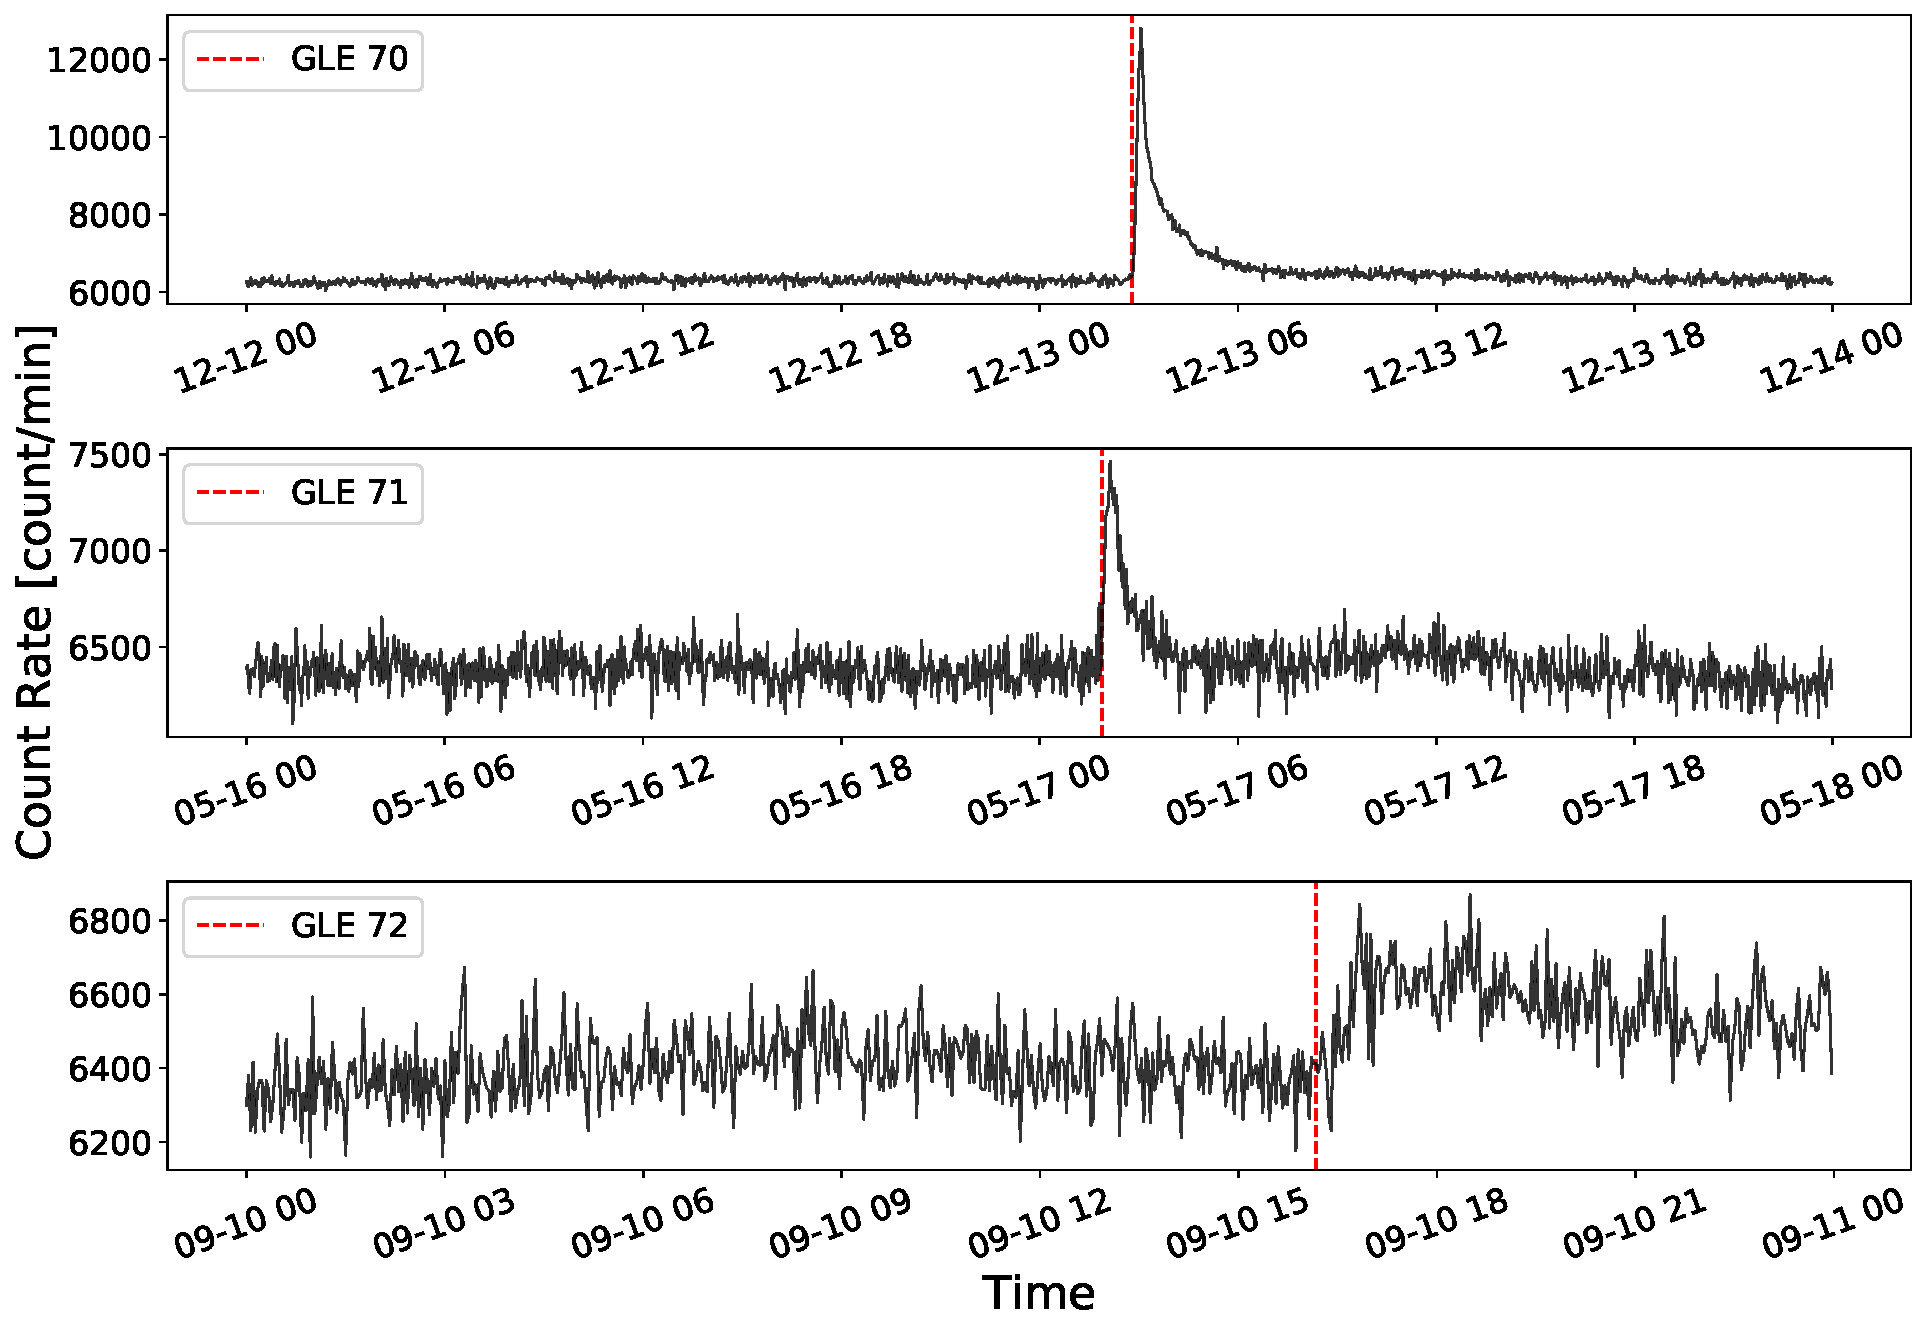
\includegraphics[width=0.75\columnwidth]{GLEs_OULU.pdf}
	\caption{GLEs observed by the NM stations based at Oulu. Top panel: GLE 70; middle panel: GLE 71, bottom panel: GLE 72. The solid-black line shows the 2-minute-averaged, pressure corrected data and the vertical, dashed-red lines show the epochs of each GLE onset. The units of time on the x-axis are, MM-DD HH.}
	\label{fig:oulu_gles}
\end{figure}

\vspace{2em}

\begin{figure}[ht!]
	\centering
	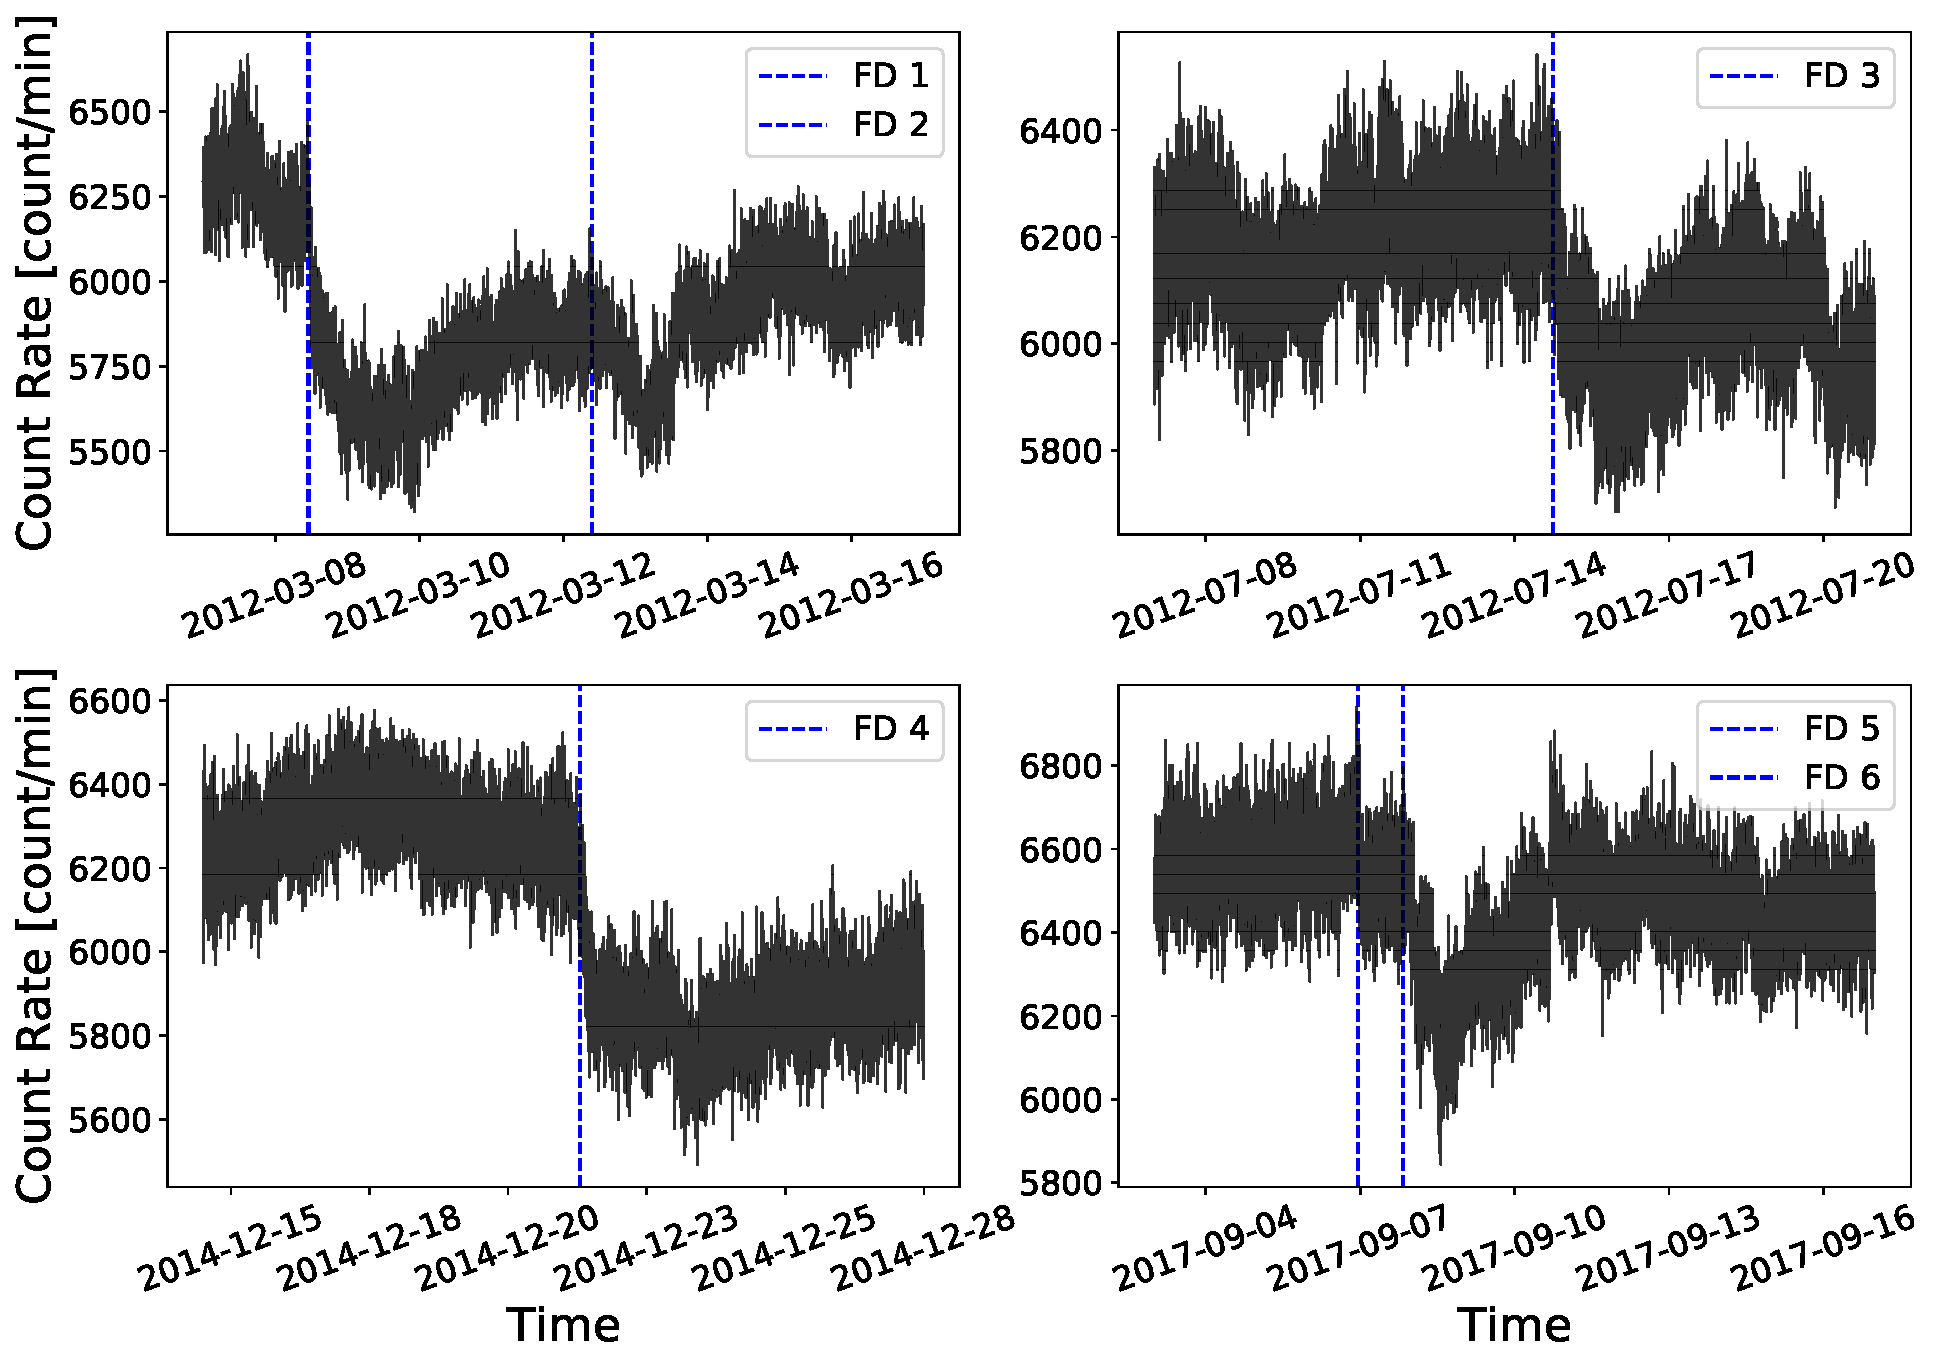
\includegraphics[width=0.75\columnwidth]{FDs_OULU.pdf}
	\caption{FDs observed by the NM stations based at Oulu. Top left panel: FDs during March 2012; top right panel: FD during July 2012; bottom left panel: FD during December 2014; bottom right panel: FD during September 2017. The solid-black line shows the 2-minute-averaged, pressure corrected data and the vertical, dashed-blue lines show the epochs of each FD onset. The units of time on the x-axis are, YYYY-MM-DD.}
	\label{fig:oulu_fds}
\end{figure}


Each \gls{fd} in Figure~\ref{fig:oulu_fds} produces a moderate decrease in the \gls{nm} count rate. The relative decreases in the the \gls{cr} counts during the \glspl{fd} were generally around $\sim 5\%$, and are easily observable by-eye in the data.





%%%%%%%%%%%%%%%%%%%%%%%%%%%%%%%%%%%%%%%%%%%%%%%%%%%%%%%%%%%%%%%%%%%%%
%%%%%%%%%%%%%%%%%%%%%%%%%%%%%%%%%%%%%%%%%%%%%%%%%%%%%%%%%%%%%%%%%%%%%
\section{Aims}\label{sec:HS_aims}


The principle aim of the project was to determine whether the existing \gls{hisparc} network is capable of observing space weather events. To do this, we initially explored the properties of the \gls{hisparc} detectors in detail, to understand the typical \glspl{pcr} they observe. In addition, we investigated the data during periods of space weather activity to search for the associated signatures detailed in Table~\ref{tab:space_weather_events}. We searched through some of the most reliable \gls{hisparc} stations to determine whether these events were observed in the data. This was done to determine whether, without much effort, we could get a binary answer on whether these events were observed by \gls{hisparc}.

Ground-based observations of muons from air showers are susceptible to the conditions in the atmosphere; where possible, we aimed to correct for these atmospheric effects and again reviewed the corrected data to determine whether the space weather events were observed.

Finally, we also aimed to perform simulations of air showers initiated by \glspl{cr} to understand the expected muon flux and dispersion at ground level. This would help us to understand how likely it is to observe the \glspl{pcr} associated with space weather with the \gls{hisparc} detectors, observing muons.

It was highlighted during private communication with the UK Met Office that observations of \glspl{gle} are of more interest and importance to space weather forecasts and nowcasts. As discussed above, using \glspl{md} generally provides observations of higher energy \glspl{pcr} which relates to the earlier onset of \glspl{sep}; thus using the \gls{hisparc} network is of significant interest in this domain. \glspl{fd} are of lower interest and importance; however, we still searched for \glspl{fd} within the \gls{hisparc} data for completeness. 


%%%%%%%%%%%%%%%%%%%%%%%%%%%%%%%%%%%%%%%%%%%%%%%%%%%%%%%%%%%%%%%%%%%%%
%%%%%%%%%%%%%%%%%%%%%%%%%%%%%%%%%%%%%%%%%%%%%%%%%%%%%%%%%%%%%%%%%%%%%
\section{HiSPARC Data}\label{sec:HS_data}


The \gls{hisparc} cosmic ray data are available on the \gls{hisparc} Public Database\footnote{\url{https://data.hisparc.nl/}}, where each station is listed, grouped by local nodes. For every station one can see its ID, name, and a coloured square and circle displaying its current data delivery and data acquisition status, respectively. Clicking on any station takes you to a dedicated page which displays its data on a user-selected day. Where data are available, it is possible to download: %The data are stored in {\verb HDF5 } format but are downloaded in {\verb .tsv } format. 
%
\begin{itemize}
	\item{events rate data: where multiple detectors in a station are triggered to satisfy that station's trigger condition;}
	\item{singles rate data: the count rates of the individual detectors within a station;}
	\item{weather data: meteorological data, including pressure and temperature;}
	\item{coincidences data: the counts where different stations measure the same event (to within $1.36 \, \upmu$s); it is possible to determine if stations measured the same event by comparing the \gls{gps} timestamps of events.}
\end{itemize}


This method of obtaining \gls{hisparc} data is acceptable if only a small quantity of data are needed, but it is cumbersome if large quantities of data are required. To obtain large quantities of \gls{hisparc} data, it was more efficient to use the \gls{esd} module within the \gls{sapphire} Python package \citep{fokkema_sapphire_2012}. The data are downloaded in the raw {\verb HDF5 } format, and can then be manipulated using further Python scripts.

A Python script was written, which used the \gls{sapphire} \gls{esd} module, to request the download of a specific type of data (i.e. events, singles, weather), from a user-specified station, download and open the {\verb HDF5 } table, manipulate the data to either keep them in the raw cadence or resample into other timebases, and finally store the data in {\verb .csv } format. This reduced the complexity involved in downloading the data and provided a repeatable method of acquiring the \gls{hisparc} data in a consistent format.

There are $\sim 140$ stations in the \gls{hisparc} network \citep{van_dam_hisparc_2020} which have been uploading data for varying durations since 2005. It was too challenging to acquire and analyse data from every station, hence a smaller sample of 5 stations was selected for investigation. The stations in the sample are outlined in Table~\ref{tab:HS_stns}, a mixture of 2-detector and 4-detector stations. Approximately 110 of the $\sim 140$ stations record singles rates, which have only been available since 2016, and only 29 stations acquire meteorological data. In general, throughout the history of the \gls{hisparc} network, the availability of weather data is irregular and many stations that acquire the data go through periods of acquiring no meteorological data at all, which made the selection of stations non-trivial. 

The 5 stations in the sample were selected as they generally have both the singles and weather data available, with the exception of station 14001 (University of Birmingham). Station 14001 only came online in 2014; it does not acquire weather data and did not begin acquiring singles data until February 2019, but it was deemed advantageous to include this station as it is maintained by the University of Birmingham, therefore we have full control over the operation of the station and it is a useful reference. Station 501 (Nikhef) is the original station in the network, and serves as the `gold standard' for \gls{hisparc}, therefore it was included. The other three stations all showed good data quality in terms of data availability and consistent operating conditions. The stations are shown on a map in Fig.~\ref{fig:HS_map}.


\begin{figure}[htbp!]
	\centering
	
\includegraphics[width=0.7\columnwidth]{HS_station_map.pdf}
	\caption{The geographic location of each HiSPARC station considered in this work. Each green circle denotes the location of a detector station.}
	\label{fig:HS_map}
\end{figure}


Figure~\ref{fig:HS_data_availability} shows the availability of \gls{cr} data from the sample of stations for each of the space weather events investigated, where purple grids denote no available data, teal denotes events data were available, and yellow denotes events and singles data were available. For each event, we have data available from at least two stations, which allows us to compare the signals. It also shows as the \gls{hisparc} network matures, so does the number of stations with available data, and the type of data available (both events and singles rates).

\begin{figure}[htbp!]
	\centering
	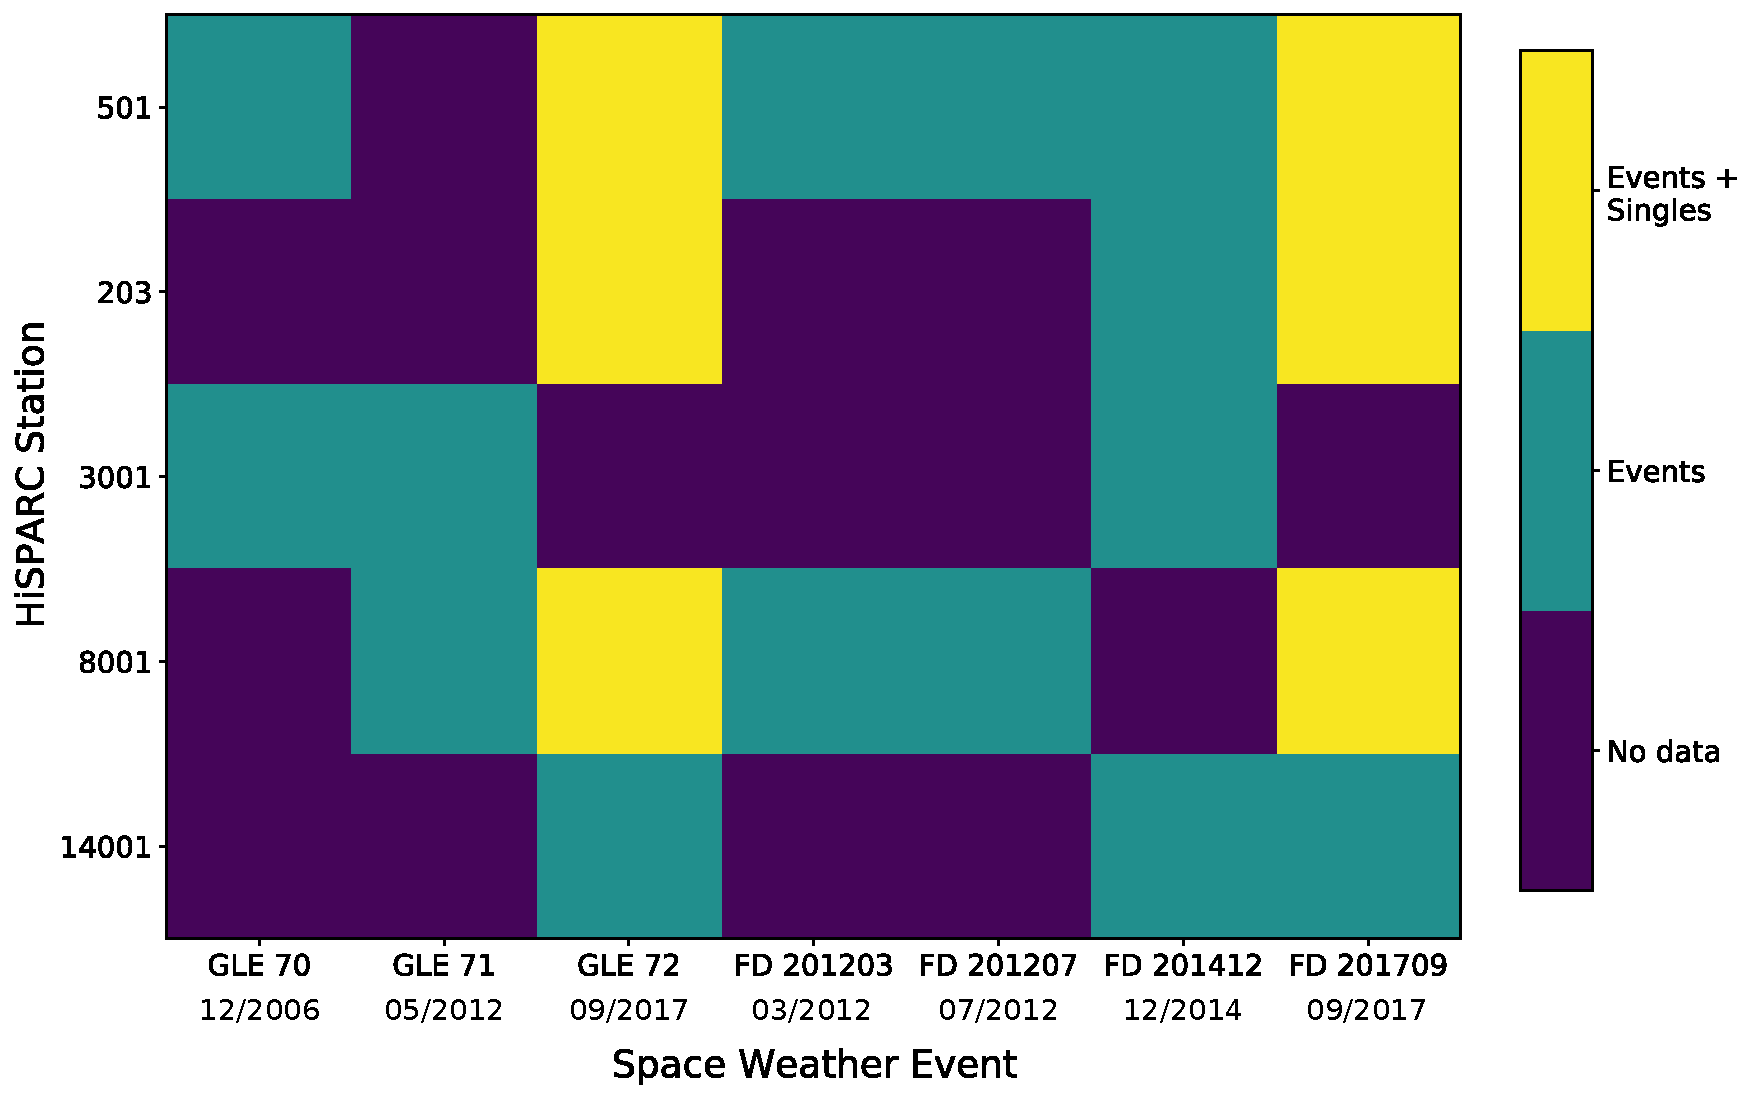
\includegraphics[width=0.85\columnwidth]{HS_data_availaviblity_map.pdf}
	\caption{The availability of data for each HiSPARC station considered, for each of the space weather epochs listed in Table~\ref{tab:space_weather_events}. The purple grids denote no available data, teal denotes that only the events data are available, and yellow denotes that both the events and singles data are available.}
	\label{fig:HS_data_availability}
\end{figure}





%%%%%%%%%%%%%%%%%%%%%%%%%%%%%%%%%%%%%%%%%%%%%%%%%%%%%%%%%%%%%%%%%%%%%
%%%%%%%%%%%%%%%%%%%%%%%%%%%%%%%%%%%%%%%%%%%%%%%%%%%%%%%%%%%%%%%%%%%%%
\section{Station Properties}\label{sec:HS_properties}

%%%%%%%%%%%%%%%%%%%%%%%%%%%%%%%%%%%%%%%%%%%%%%%%%%%%%%%%%%%%%%%%%%%%%
\subsection{Cut-Off Rigidity}

To understand the \gls{pcr} spectrum that ground-based \gls{cr} detectors may observe, \gls{pcr} transport simulations are typically performed \citep{mccracken_trajectories_1962,plainaki_neutron_2009,danilova_mapping_2019}. The geomagnetic field can prohibit \gls{cr} particles from penetrating the magnetosphere and reaching the atmosphere, depending on the particle's energy. As a consequence, the cut-off rigidity is an estimate of the lower rigidity-threshold, below which the particle flux is zero due to geomagnetic shielding (measured in Volts, V, or Gigavolts, GV) \citep{shea_study_1965, danilova_mapping_2019}. Transport simulations allow us to determine the range of \glspl{pcr} that have sufficient energy to penetrate the Earth's magnetosphere, which reach the atmosphere and produce secondary particle air showers. The \gls{pcr} spectrum depends strongly on the geographic location of the station; the minimum allowed particle rigidity varies from $\sim 17$~GV near the equator and theoretically 0~GV at the poles, and the geomagnetic conditions have a strong impact on the \gls{pcr} spectrum \citep{shea_study_1965, cramp_modelling_1996, desorgher_planetocosmics_2006, danilova_mapping_2019}. 

Transport simulations typically run a reverse evolution of particles, using a backwards-tracing routine, whereby the particles are simulated from Earth out to the magnetosphere, to determine whether they leave the magnetosphere or remain trapped due to the geomagnetic field \citep{shea_study_1965}. In this work, to perform the \gls{pcr} transport simulations we used the PLANETOCOSMICS software \citep{desorgher_planetocosmics_2005}. PLANETOCOSMICS performs Geant4 Monte Carlo simulations of charged particle transport through Earth's magnetosphere based on St\"{o}rmers transport equation for charged particles \citep{desorgher_planetocosmics_2005, desorgher_planetocosmics_2006}. 

PLANETOCOSMICS simulates backward trajectories of charged particles from a given location (latitude, longitude, and altitude) out to the magnetopause for a set of \gls{pcr} rigidities. For each simulated trajectory there are two possible outcomes: (i) the particles trace out to the magnetopause where they escape Earth's magnetosphere, an allowed trajectory; (ii) the particles are sufficiently bent by the effect of the Earth's magnetosphere that they do not reach the magnetopause and cannot escape the Earth's magnetosphere, a forbidden trajectory \citep{shea_study_1965, desorgher_planetocosmics_2005, desorgher_planetocosmics_2006}. The coordinates of the asymptotic direction at the magnetosphere are provided as an output from the simulations. This is the direction of motion of particles upon leaving the magnetosphere, if subjected to no other forces \citep{shea_study_1965, desorgher_planetocosmics_2006, danilova_mapping_2019}. In this work PLANETOCOSMICS was configured with the Tsyganenko-89 model for the external magnetospheric magnetic field \citep{tsyganenko_magnetospheric_1989, tsyganenko_data-based_2013} and the \gls{igrf} internal field model \citep{thebault_international_2015}.

Each simulated rigidity, whether it followed an allowed or forbidden trajectory, was stored and was used to provide an insight into the rigidity spectrum for a given station. From the allowed trajectories the effective cut-off rigidity ($R_C$) for the stations was computed, which represents the lower rigidity limit above which cosmic rays can cross the magnetosphere and reach the atmosphere:

\begin{equation}
\label{eq:cut_off}
R_C = R_U - \sum_{i = R_L}^{R_U} \Delta R_i
\end{equation}
%
where $R_U$ is the upper rigidity (the last allowed trajectory before the first forbidden trajectory); $R_L$ is the lower rigidity (the last allowed trajectory before which all other trajectories with a lower rigidity are forbidden); $\Delta R$ is the rigidity step size in the simulation \citep{shea_study_1965, desorgher_planetocosmics_2005, desorgher_planetocosmics_2006, herbst_influence_2013}.

The rigidity spectrum for each of the five \gls{hisparc} stations was investigated to determine $R_C$ for each station. The cut-off rigidity calculated for the five \gls{hisparc} stations for a vertical incidence upon the atmosphere (i.e. $0^\circ$ zenith angle) are presented in Table~\ref{tab:HS_stns} which show that there is little variation in $R_C$ between the \gls{hisparc} stations and that they observe \glspl{pcr} with rigidities in excess of $\sim 3$~GV. This analysis was initially carried out for the vertical direction (i.e. azimuth = $0^\circ$, zenith = $0^\circ$); however further trajectories were simulated for different azimuth and zenith angles to determine the dependence of the rigidity spectrum on the detector acceptance angle. The analysis for the azimuthal dependence was carried out at a zenith angle of $20^\circ$ as this is around the most probable angle for \gls{hisparc} events \citep{fokkema_hisparc_2012}, and the analysis of the zenith dependence was carried out at an azimuth angle of $0^\circ$. This analysis is shown in Figure~\ref{fig:R_C2}, and demonstrates that there is no strong dependence of the azimuth direction or zenith (up to $45^{\circ}$).


\begin{table}
	\begin{center}
		\caption{Properties of some of the HiSPARC stations: geographic longitude ($\phi$), geographic latitude ($\lambda$), altitude ($h$), and the geomagnetic vertical cut-off rigidity ($R_C$) calculated from the PLANETOCOSMICS simulations.}
		\label{tab:HS_stns}
		\begin{tabular}{l c c c c c}
			\hline
			& $R_C$  & $\phi$ & $\lambda$  & $h$  & No. Detectors\\
			Station Name/ID & [GV] & [deg] & [deg] & [m]  & \\
			\hline
			Nikhef/501 & 3.19 & 4.95 E & 52.36 N & 56.18 & 4 \\
			College Hageveld/203 & 3.18 & 4.63 E  & 52.35 N & 53.71  & 2 \\
			Leiden/3001 & 3.23 & 4.45 E & 52.17 N & 54.08 & 2 \\
			Eindhoven/8001  & 3.44 & 5.49 E & 51.45 N & 70.12 & 2 \\
			Birmingham University/14001  & 3.06 & 1.93 W & 52.45 N & 204.14 & 4  \\
			%20003 & 2.30 & 10.20 E & 56.17 N & 84.38 & 2 \\
			\hline
		\end{tabular}
	\end{center}
\end{table}

\begin{figure}[h]
	\centering
	\subfloat[Azimuth variation (fixed zenith = $20^\circ$)]{
		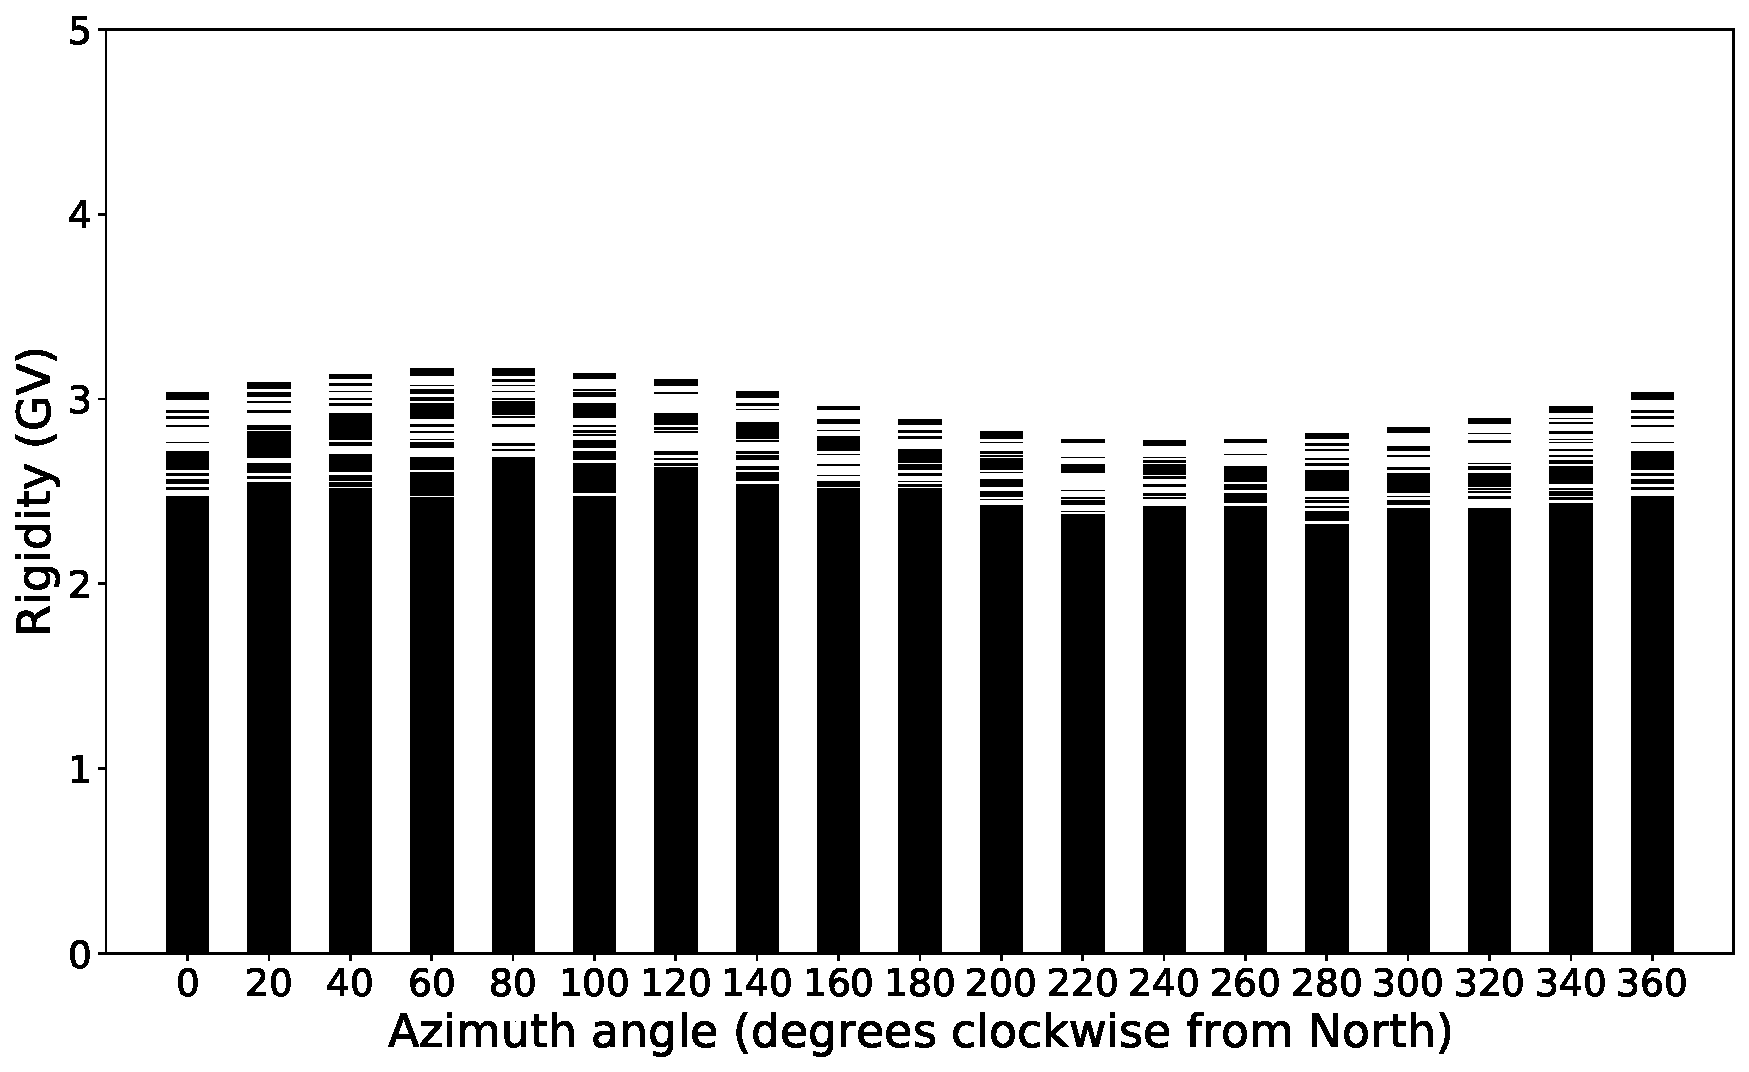
\includegraphics[width=0.48\columnwidth]{azm.pdf}
		\label{fig:azm1}}
	%\qquad
	\subfloat[Zenith variation (fixed azimuth = $0^\circ$)]{
		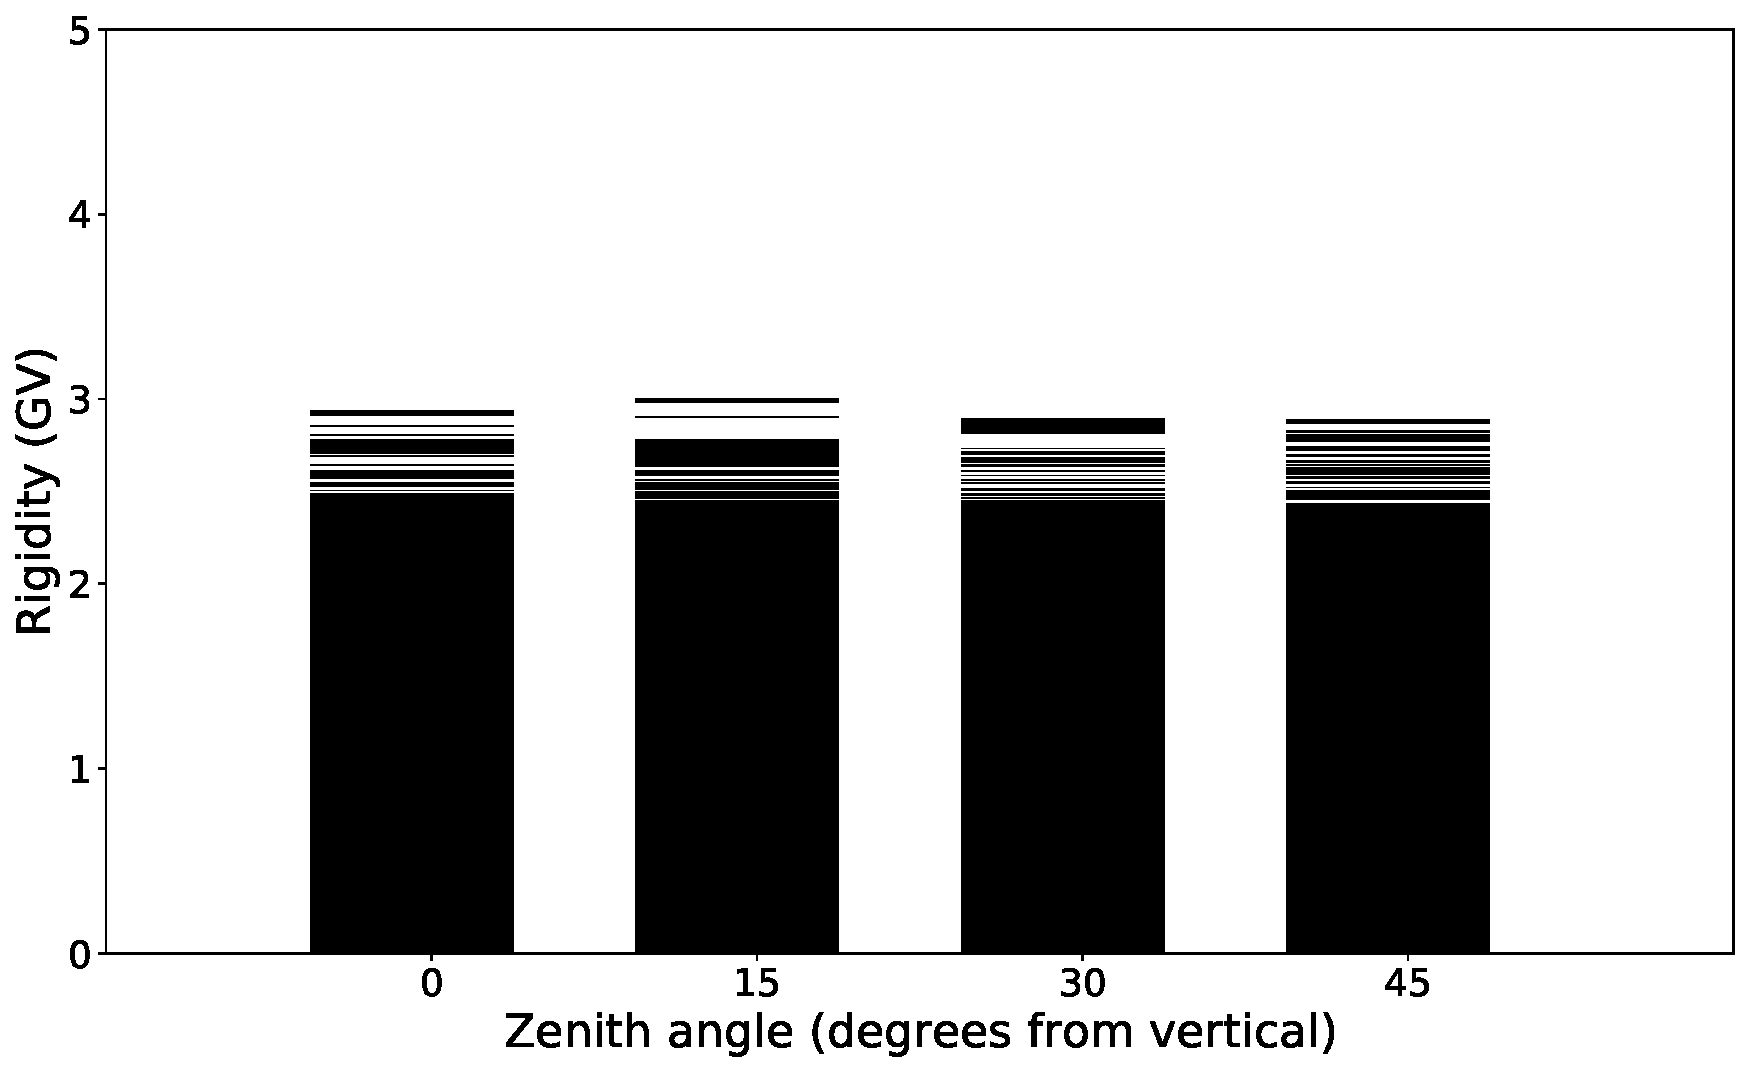
\includegraphics[width=0.48\columnwidth]{zen.pdf}
		\label{fig:zen1}}
	
	\caption{Azimuthal and zenith angle variations in the allowed and forbidden rigidity trajectories for HiSPARC station 501 from simulations in steps of rigidity, $\Delta R = 0.01$~GV. The forbidden trajectories are in black; allowed trajectories are in white.}
	\label{fig:R_C2}
\end{figure}

The small variation between \gls{hisparc} stations is due to their close proximity in geographic latitude and longitude. The values of $R_C$ calculated for the \gls{hisparc} stations suggest that they should be able to observe higher energy \glspl{scr}, but may not be as susceptible as the higher latitude \glspl{nm} where the effects of \glspl{gle} are highly observable.

%%%%%%%%%%%%%%%%%%%%%%%%%%%%%%%%%%%%%%%%%%%%%%%%%%%%%%%%%%%%%%%%%%%%%
\subsection{Asymptotic Viewing Directions}

Another output from the PLANETOCOSMICS simulations allowed us to understand the directions of moving particles entering the Earth's magnetosphere prior to their trajectory through the magnetosphere and arrival at the atmosphere. By tracking particle trajectories we can define the \gls{avd} of \gls{cr} stations, which represents the direction of \gls{cr} motion before entering the magnetosphere and being observed by a detector \citep{mccracken_trajectories_1962,danilova_mapping_2019}. This allowed us to understand the average directions in space that ground-based \gls{cr} detectors observe. Higher energy \glspl{cr} are deflected less by the magnetosphere and therefore the \glspl{avd} of high rigidity cut-off stations are simply their zenith; however, lower energy \glspl{cr} are deflected more, there stations with a lower rigidity cut-off may observe \glspl{cr} from a range of directions.

It can be seen from Figure~\ref{fig:HS_AVD} that the \glspl{avd} for each of the \gls{hisparc} stations investigated are rather similar, due to their close geographic proximity, and that they mostly straddle the equator for low rigidity \glspl{pcr}. 

\begin{figure}[ht!]
	\centering
	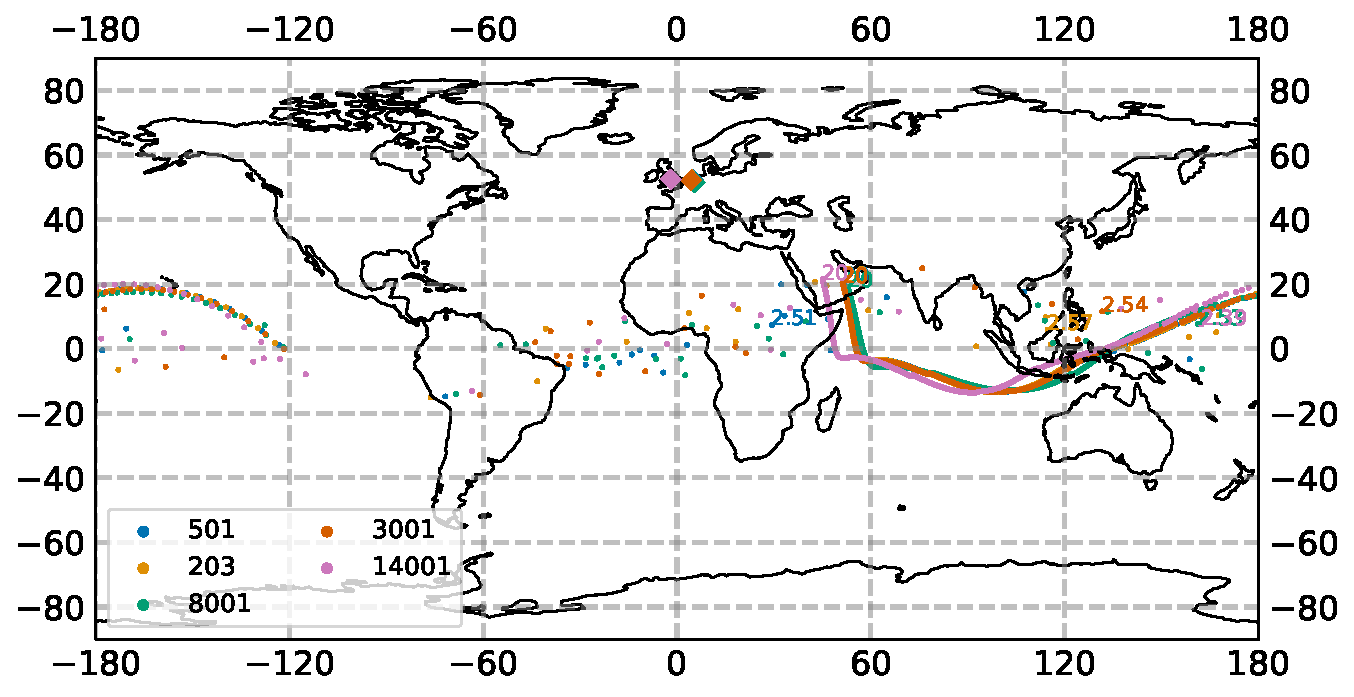
\includegraphics[scale=0.6]{HS_AVDs.pdf}
	\caption{The vertical asymptotic viewing directions of 5 HiSPARC stations. The rigidity range of the simulations were from $1.0$~GV $<$ R $<20.0$~GV, and the results are plotted in geographic coordinates on January 20th 2005. The diamonds correspond to the HS ground location and the circles correspond to the AVD for a specific rigidity value.}
	\label{fig:HS_AVD}
\end{figure}

The simulations were performed up to a rigidity of 20~GV, in steps of $\Delta R = 0.01$~GV, and the \glspl{avd} are limited between $\pm 20^{\circ}$ latitude. However, at higher rigidities, we would see the \glspl{avd} spiral in towards the geographic location of the station and the \gls{pcr} would enter the magnetosphere and atmosphere almost vertically above the detector. The 20~GV directions are all grouped closely together due to the close geographic locations of the stations. This map of the \glspl{avd} also informs us that we should expect to be able to observe some lower energy \glspl{pcr} when the zenith of the detector is not facing the asymptotic direction of the \gls{pcr}. The viewing directions of allowed, lower rigidity, trajectories with $R_C \sim 2.5$~GV are shifted easterly by $\sim 120^{\circ}$ longitude. This demonstrates that the observable, lower-energy \glspl{pcr} are deflected significantly by the Earth's magnetosphere; we can therefore detect solar eruptive events when the station is not pointing in a direction in-line with the Sun and hence observe \glspl{sep} $\sim 8$~hours before the stations align with the direction of the source.


This has a significant impact on the ability of the \gls{hisparc} detectors to observe transient solar eruptive events which have a \gls{sep} spectrum with energies $<10^9$~eV. In addition, the ability of \gls{hisparc} to observe highly anisotropic events may be limited because of the similar \glspl{avd} for all the \gls{hisparc} stations. For this latter reason, many ground-based \gls{cr} stations are spread across Earth's surface, to maximise the observation coverage.


%%%%%%%%%%%%%%%%%%%%%%%%%%%%%%%%%%%%%%%%%%%%%%%%%%%%%%%%%%%%%%%%%%%%%
%%%%%%%%%%%%%%%%%%%%%%%%%%%%%%%%%%%%%%%%%%%%%%%%%%%%%%%%%%%%%%%%%%%%%
\section{HiSPARC Observations}\label{sec:HS_obs}


%%%%%%%%%%%%%%%%%%%%%%%%%%%%%%%%%%%%%%%%%%%%%%%%%%%%%%%%%%%%%%%%%%%%%
\subsection{Observations of Ground Level Enhancements}

The search for evidence of \glspl{gle} within the \gls{hisparc} data was conducted for the events listed in Table~\ref{tab:space_weather_events}, as they are the only \glspl{gle} that span the operational epoch of the \gls{hisparc} network. Figures~\ref{fig:GLE_70}, ~\ref{fig:GLE_71}, and ~\ref{fig:GLE_72} show the \gls{hisparc} observations around \gls{gle} 70, 71, and 72, respectively. As highlighted by Fig.~\ref{fig:HS_data_availability}, most of the observations are only the events data (i.e. coincidences between the detectors of a station); however, where possible, we also show the singles rates from each of the individual detectors in a station, when available.

\begin{figure}[ht!]
	\centering
	\subfloat[HS 501 (Nikhef)]{
		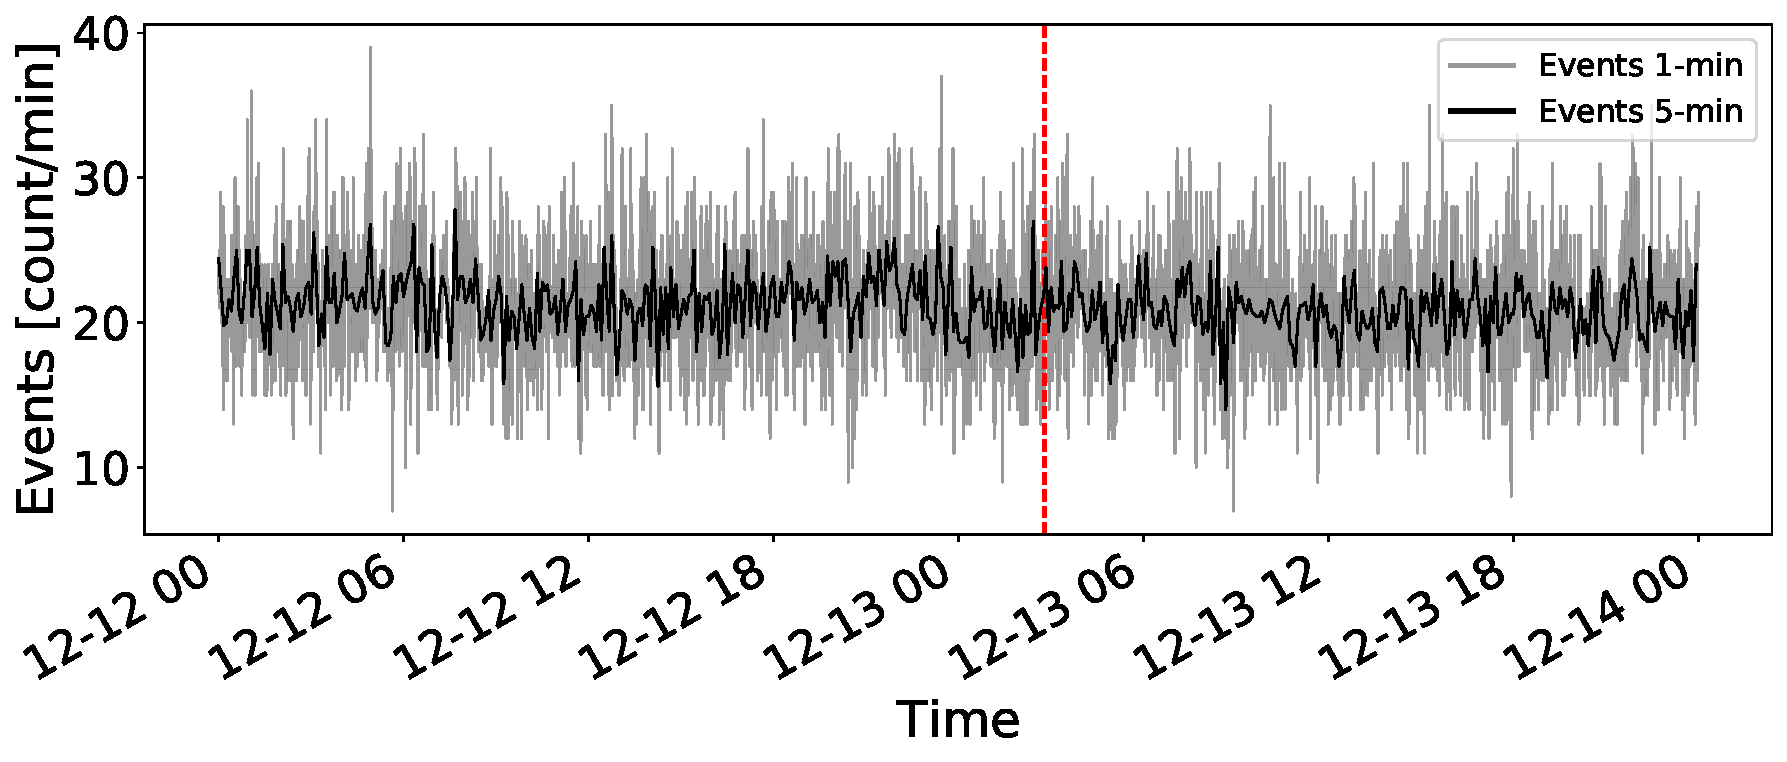
\includegraphics[width=0.48\columnwidth]{GLE70_501.pdf}
		\label{fig:GLE70_501}}
	%\qquad
	\subfloat[HS 3001 (Universiteit Leiden)]{
		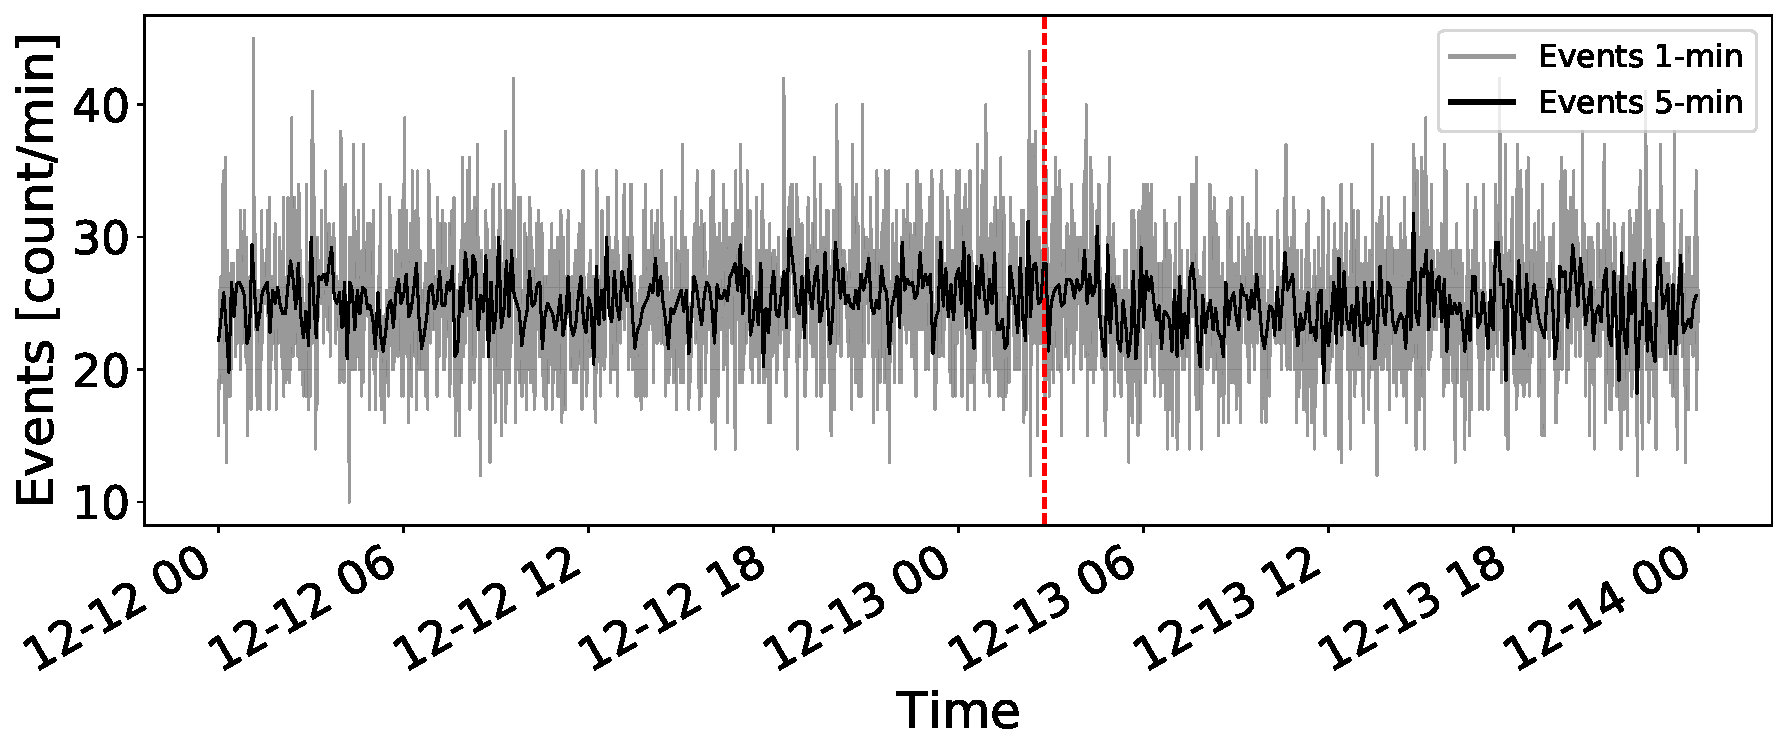
\includegraphics[width=0.48\columnwidth]{GLE70_3001.pdf}
		\label{fig:GLE70_3001}}
	
	\caption{HiSPARC data for stations 501 and 3001 around the epoch of GLE 70 on 13/12/2006. The plot shows the minute-averaged (grey) and 5-minute-averaged (black) trigger events between detectors within the station. The vertical red, dashed line depicts the approximate onset time of the GLE. The units of time on the x-axis are, MM-DD HH.}
	\label{fig:GLE_70}
\end{figure}

\begin{figure}[ht!]
	\centering
	\subfloat[HS 8001 (Eindhoven)]{
		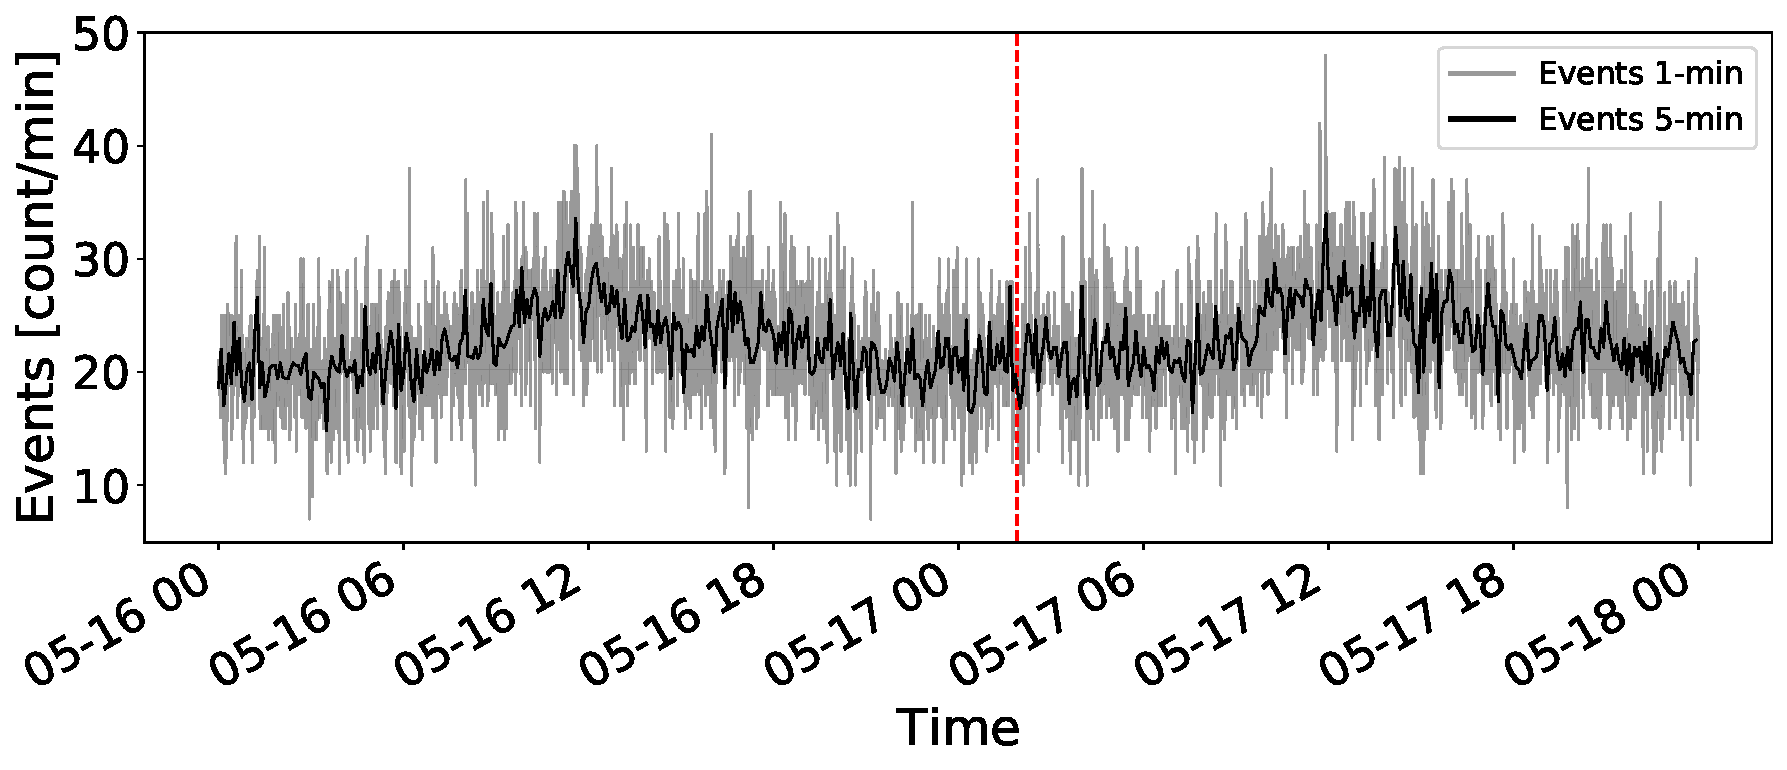
\includegraphics[width=0.48\columnwidth]{GLE71_8001.pdf}
		\label{fig:GLE71_8001}}
	%\qquad
	\subfloat[HS 3001 (Universiteit Leiden)]{
		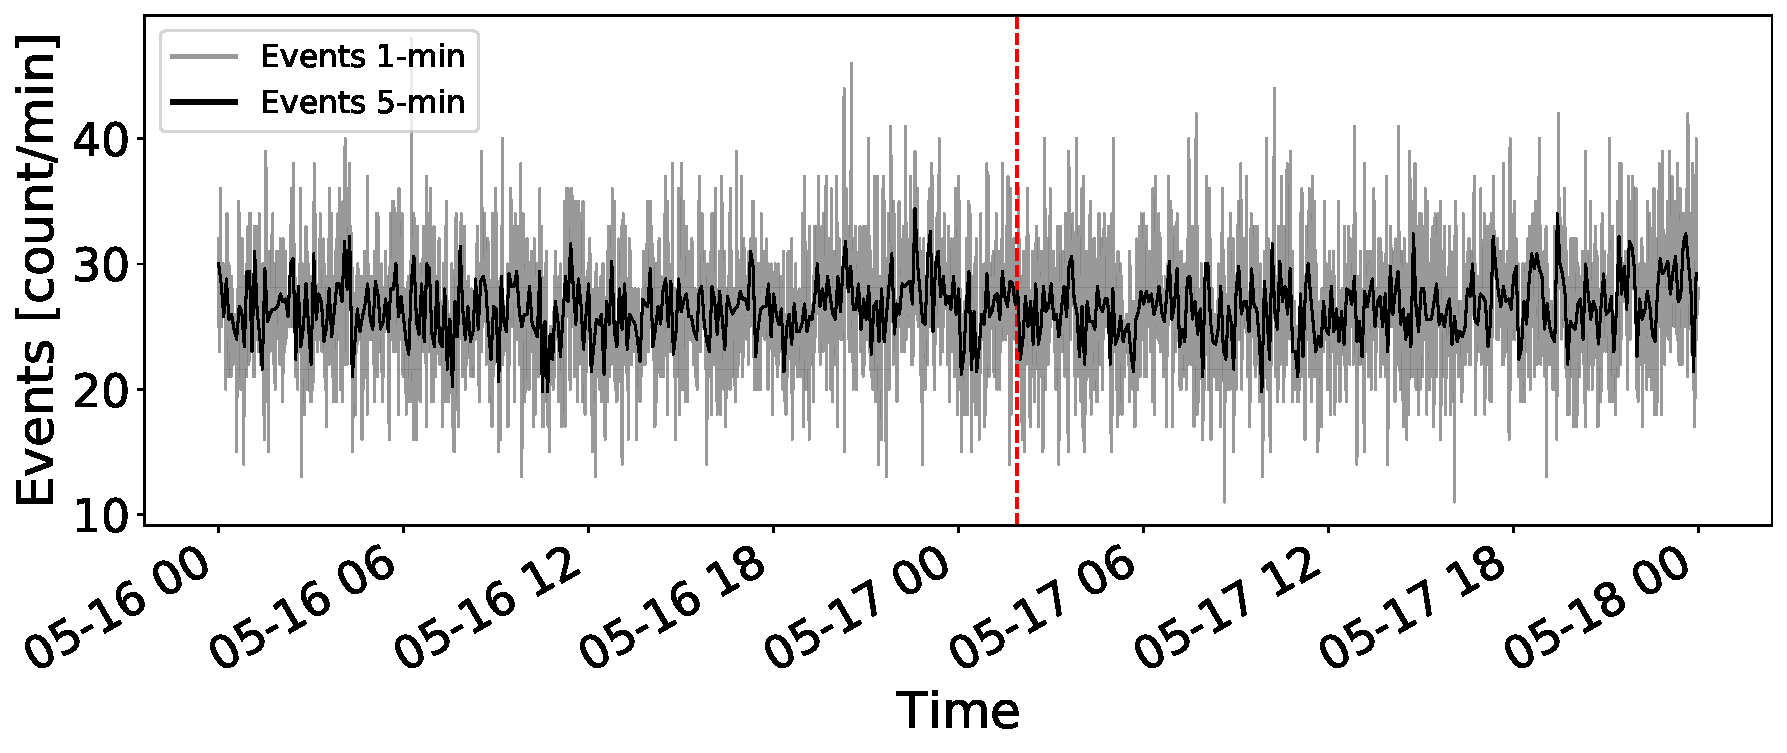
\includegraphics[width=0.48\columnwidth]{GLE71_3001.pdf}
		\label{fig:GLE71_3001}}
	
	\caption{HiSPARC data for stations 8001 and 3001 around the epoch of GLE 71 on 17/05/2012. The plot shows the minute-averaged (grey) and 5-minute-averaged (black) trigger events between detectors within the station. The vertical red, dashed line depicts the approximate onset time of the GLE. The units of time on the x-axis are, MM-DD HH.}
	\label{fig:GLE_71}
\end{figure}

\begin{figure}[ht!]
	\centering
	\subfloat[HS 501 (Nikhef)]{
		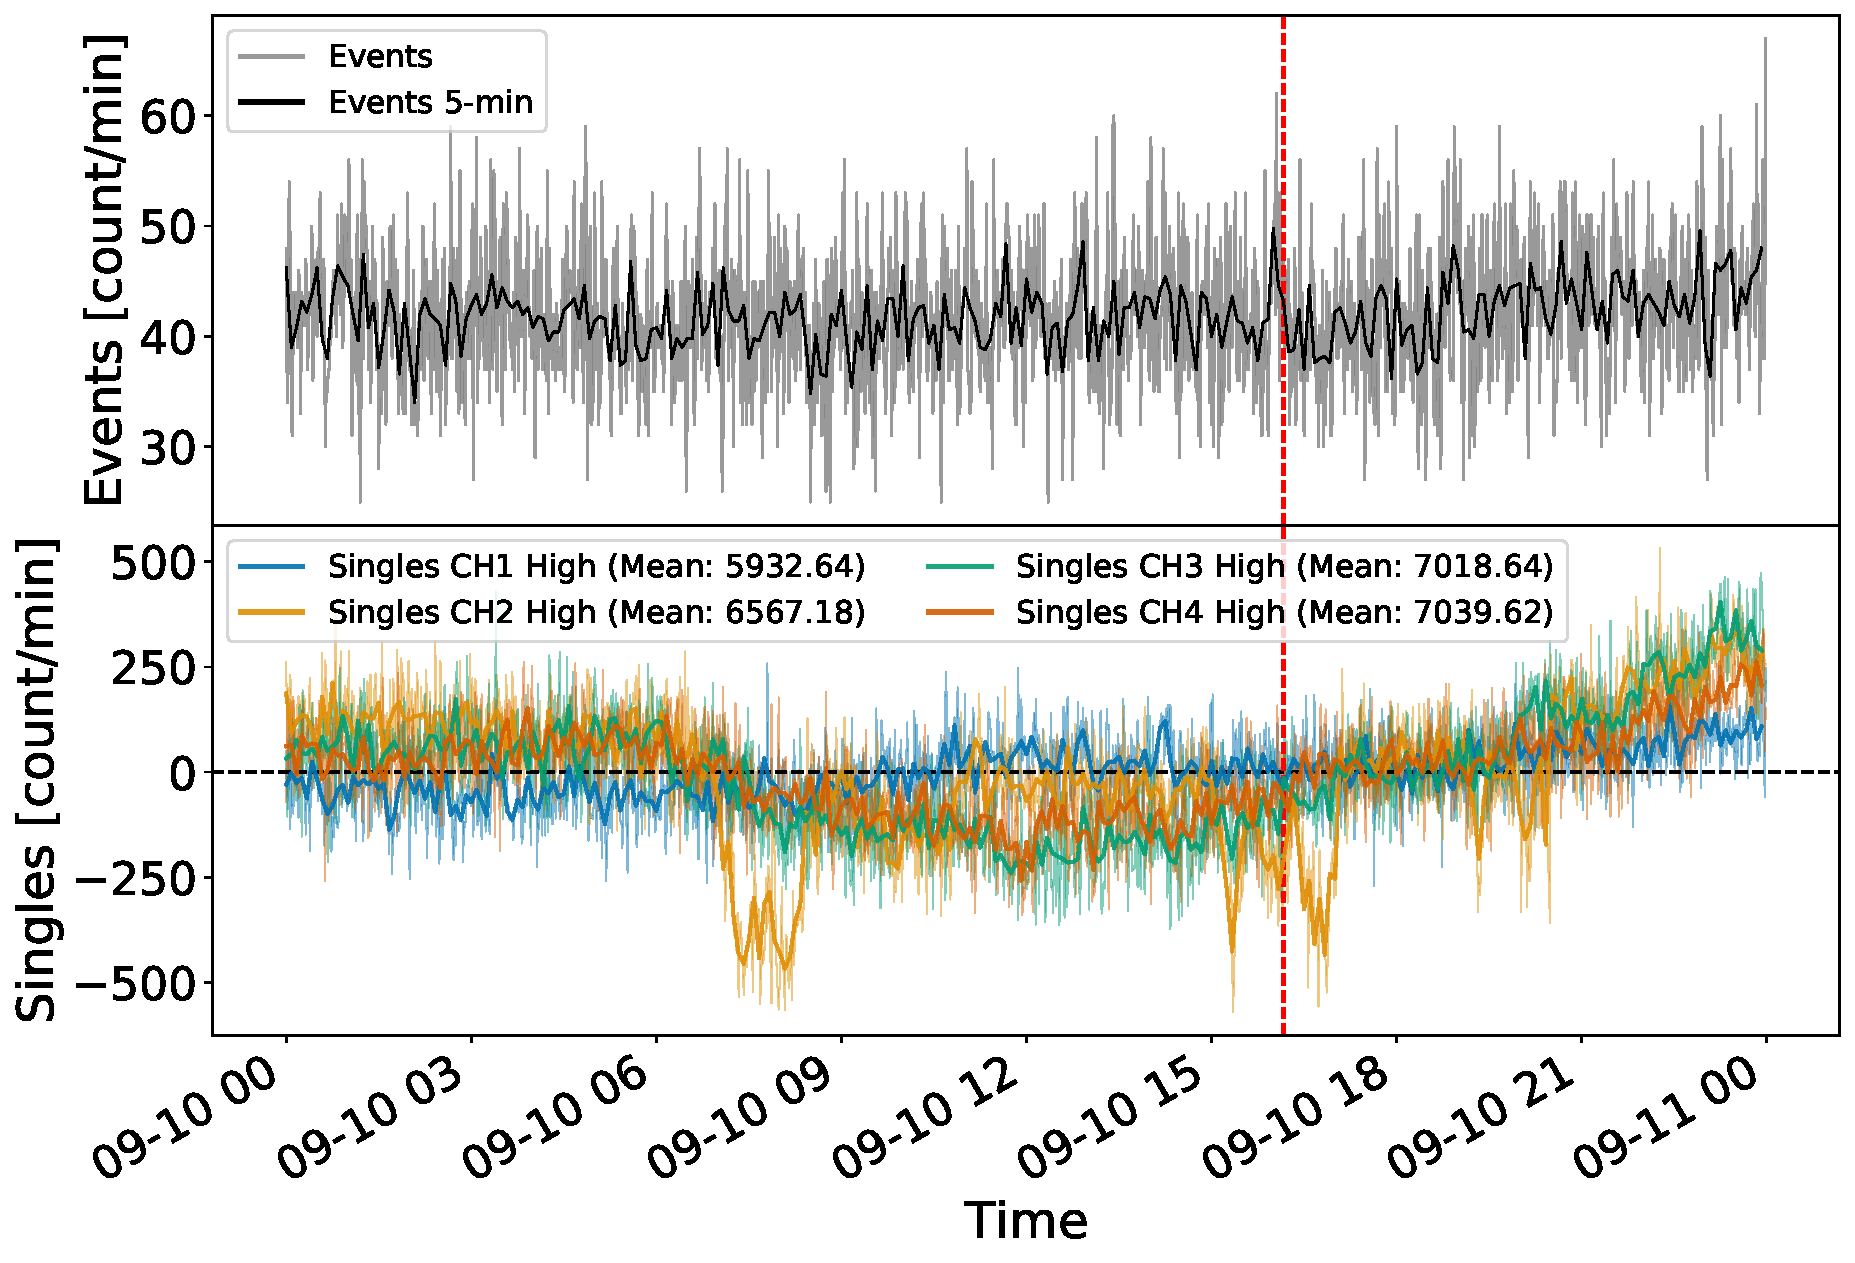
\includegraphics[width=0.48\columnwidth]{GLE72_501.pdf}
		\label{fig:GLE72_501}}
	%\qquad
	\subfloat[HS 203 (College Hageveld)]{
		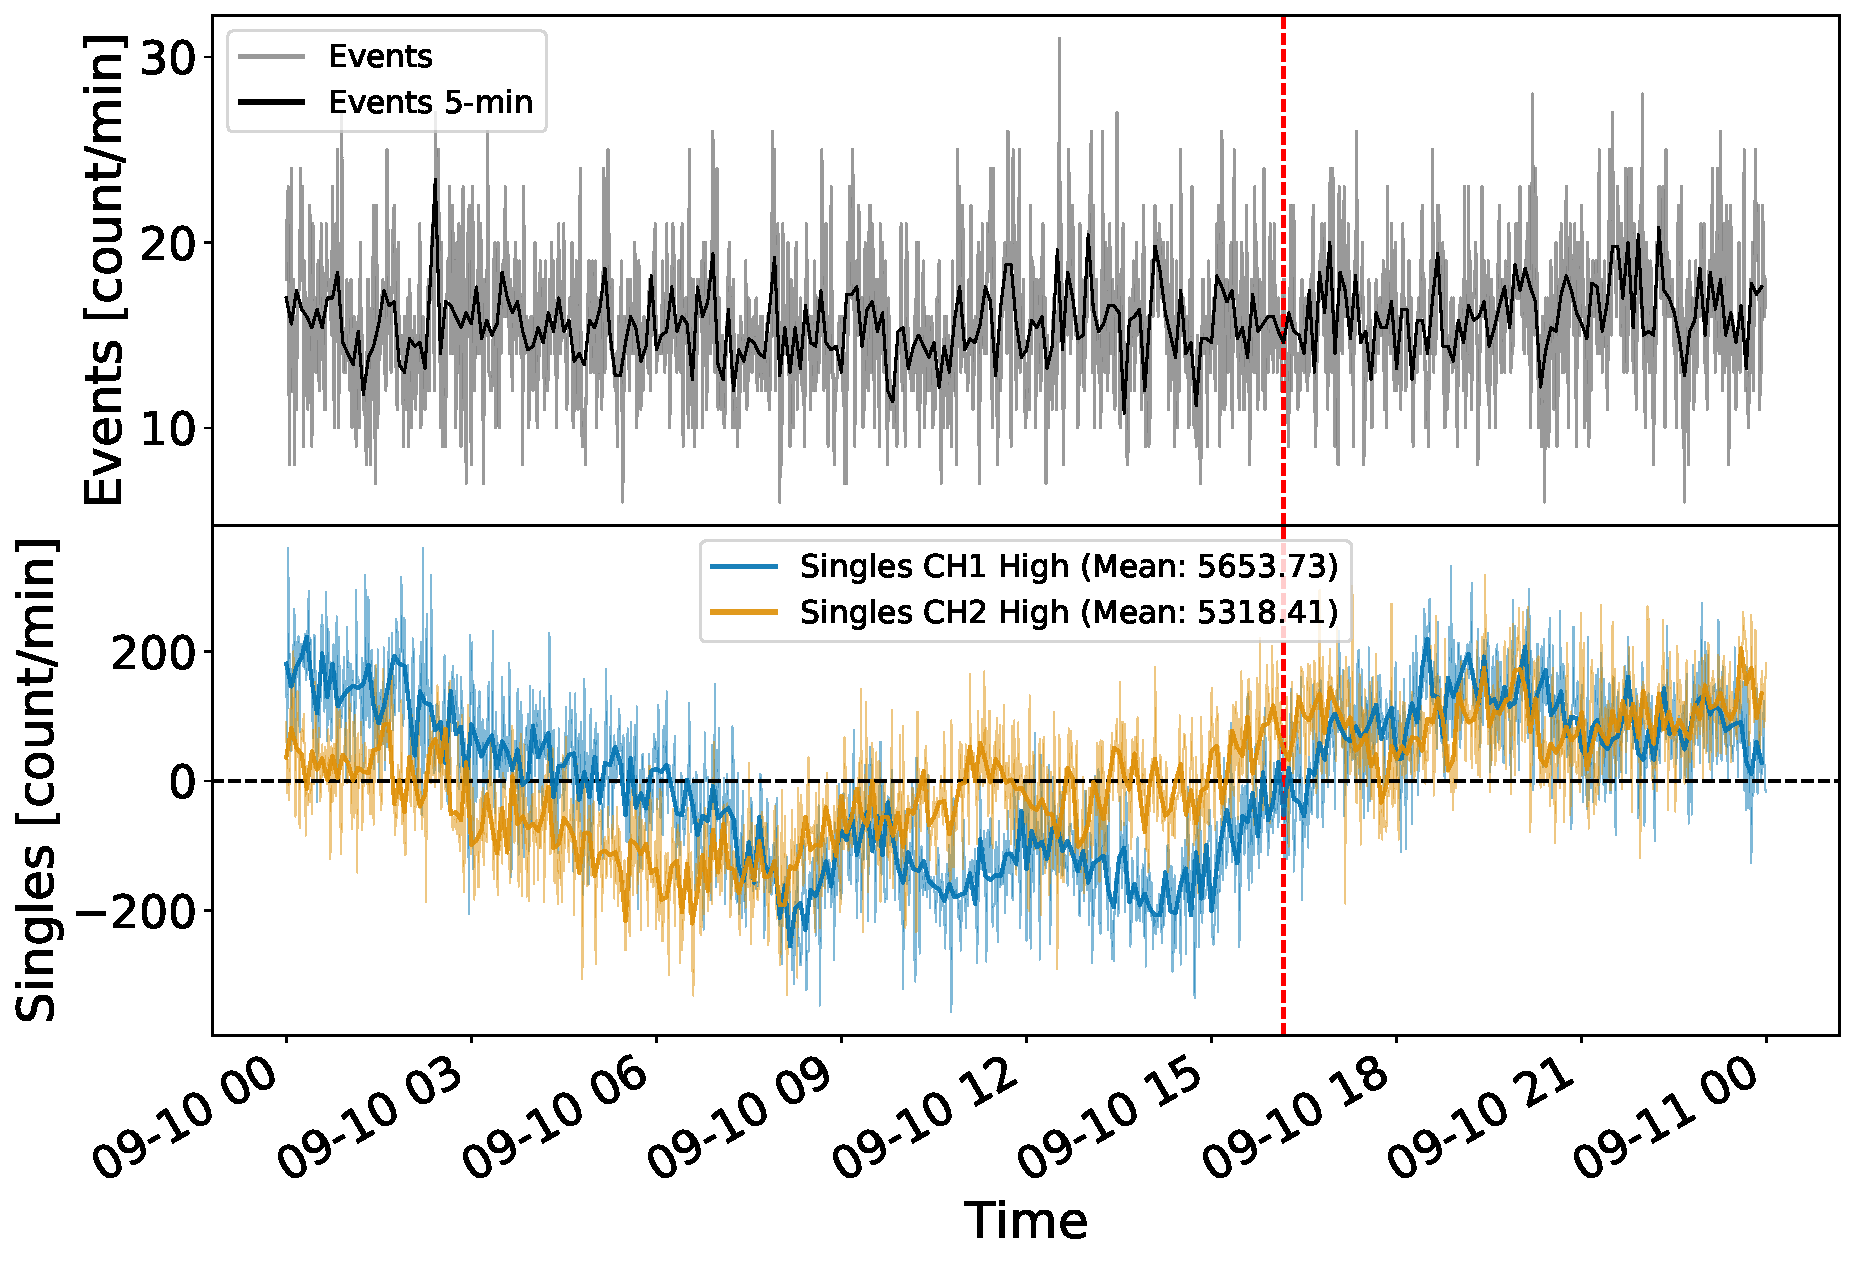
\includegraphics[width=0.48\columnwidth]{GLE72_203.pdf}
		\label{fig:GLE72_203}} \\
	
	\qquad
	
	\subfloat[HS 8001 (Eindhoven)]{
		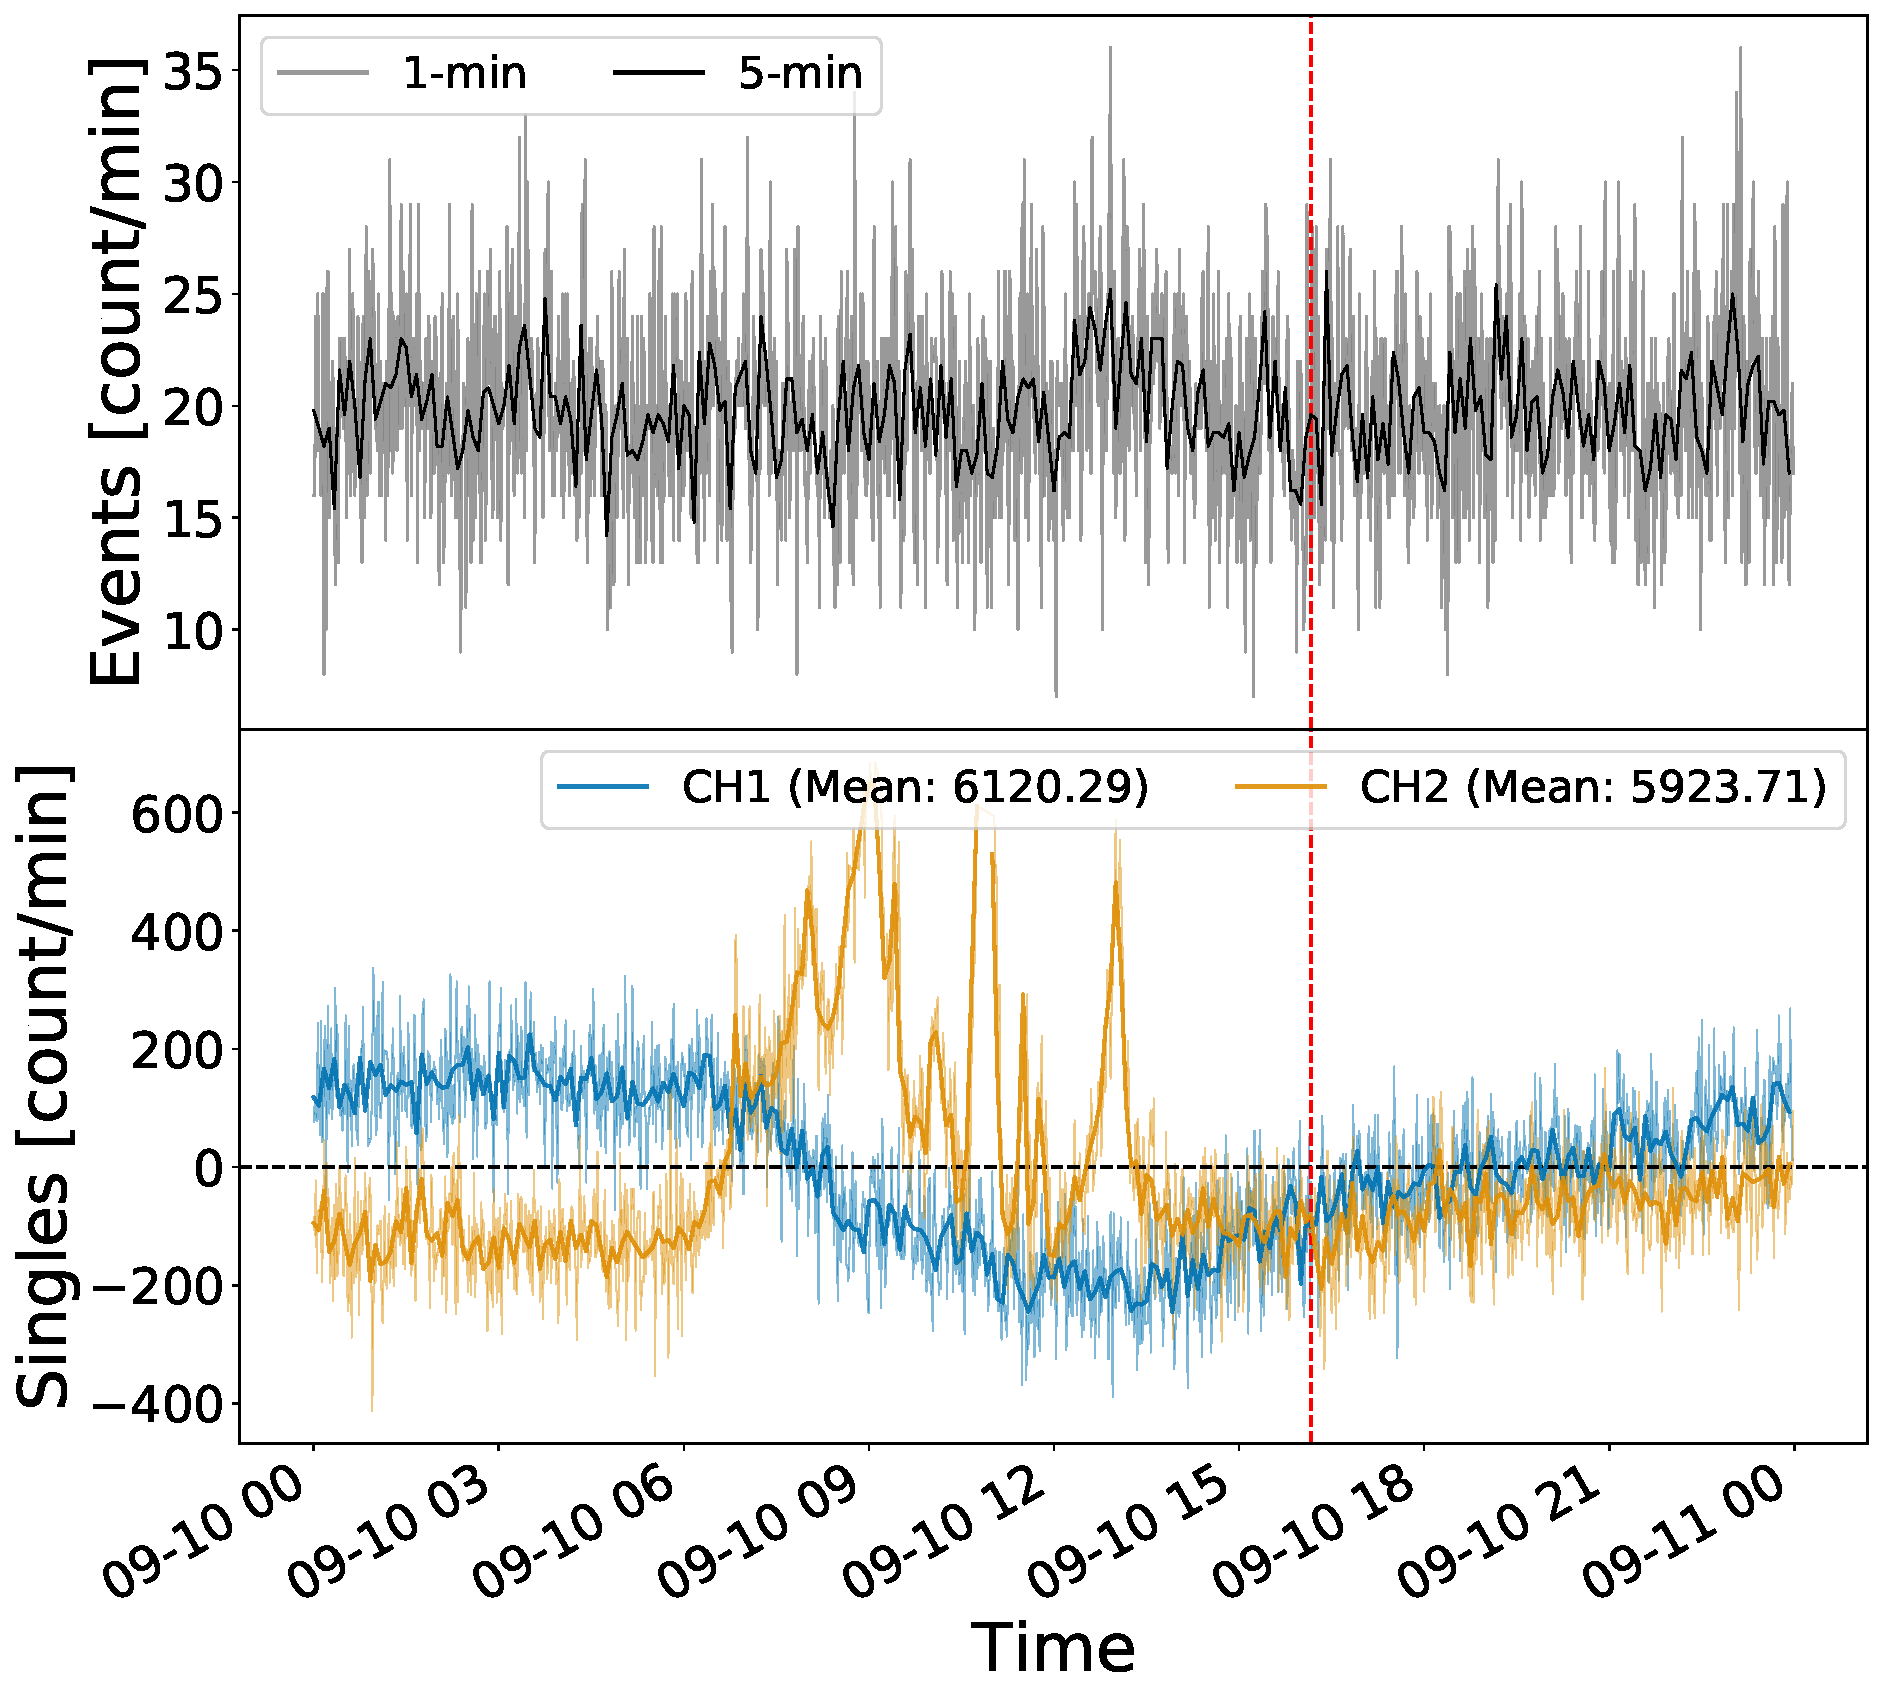
\includegraphics[width=0.48\columnwidth]{GLE72_8001.pdf}
		\label{fig:GLE72_8001}}
	%\qquad
	\subfloat[HS 14001 (Birmingham University)]{
		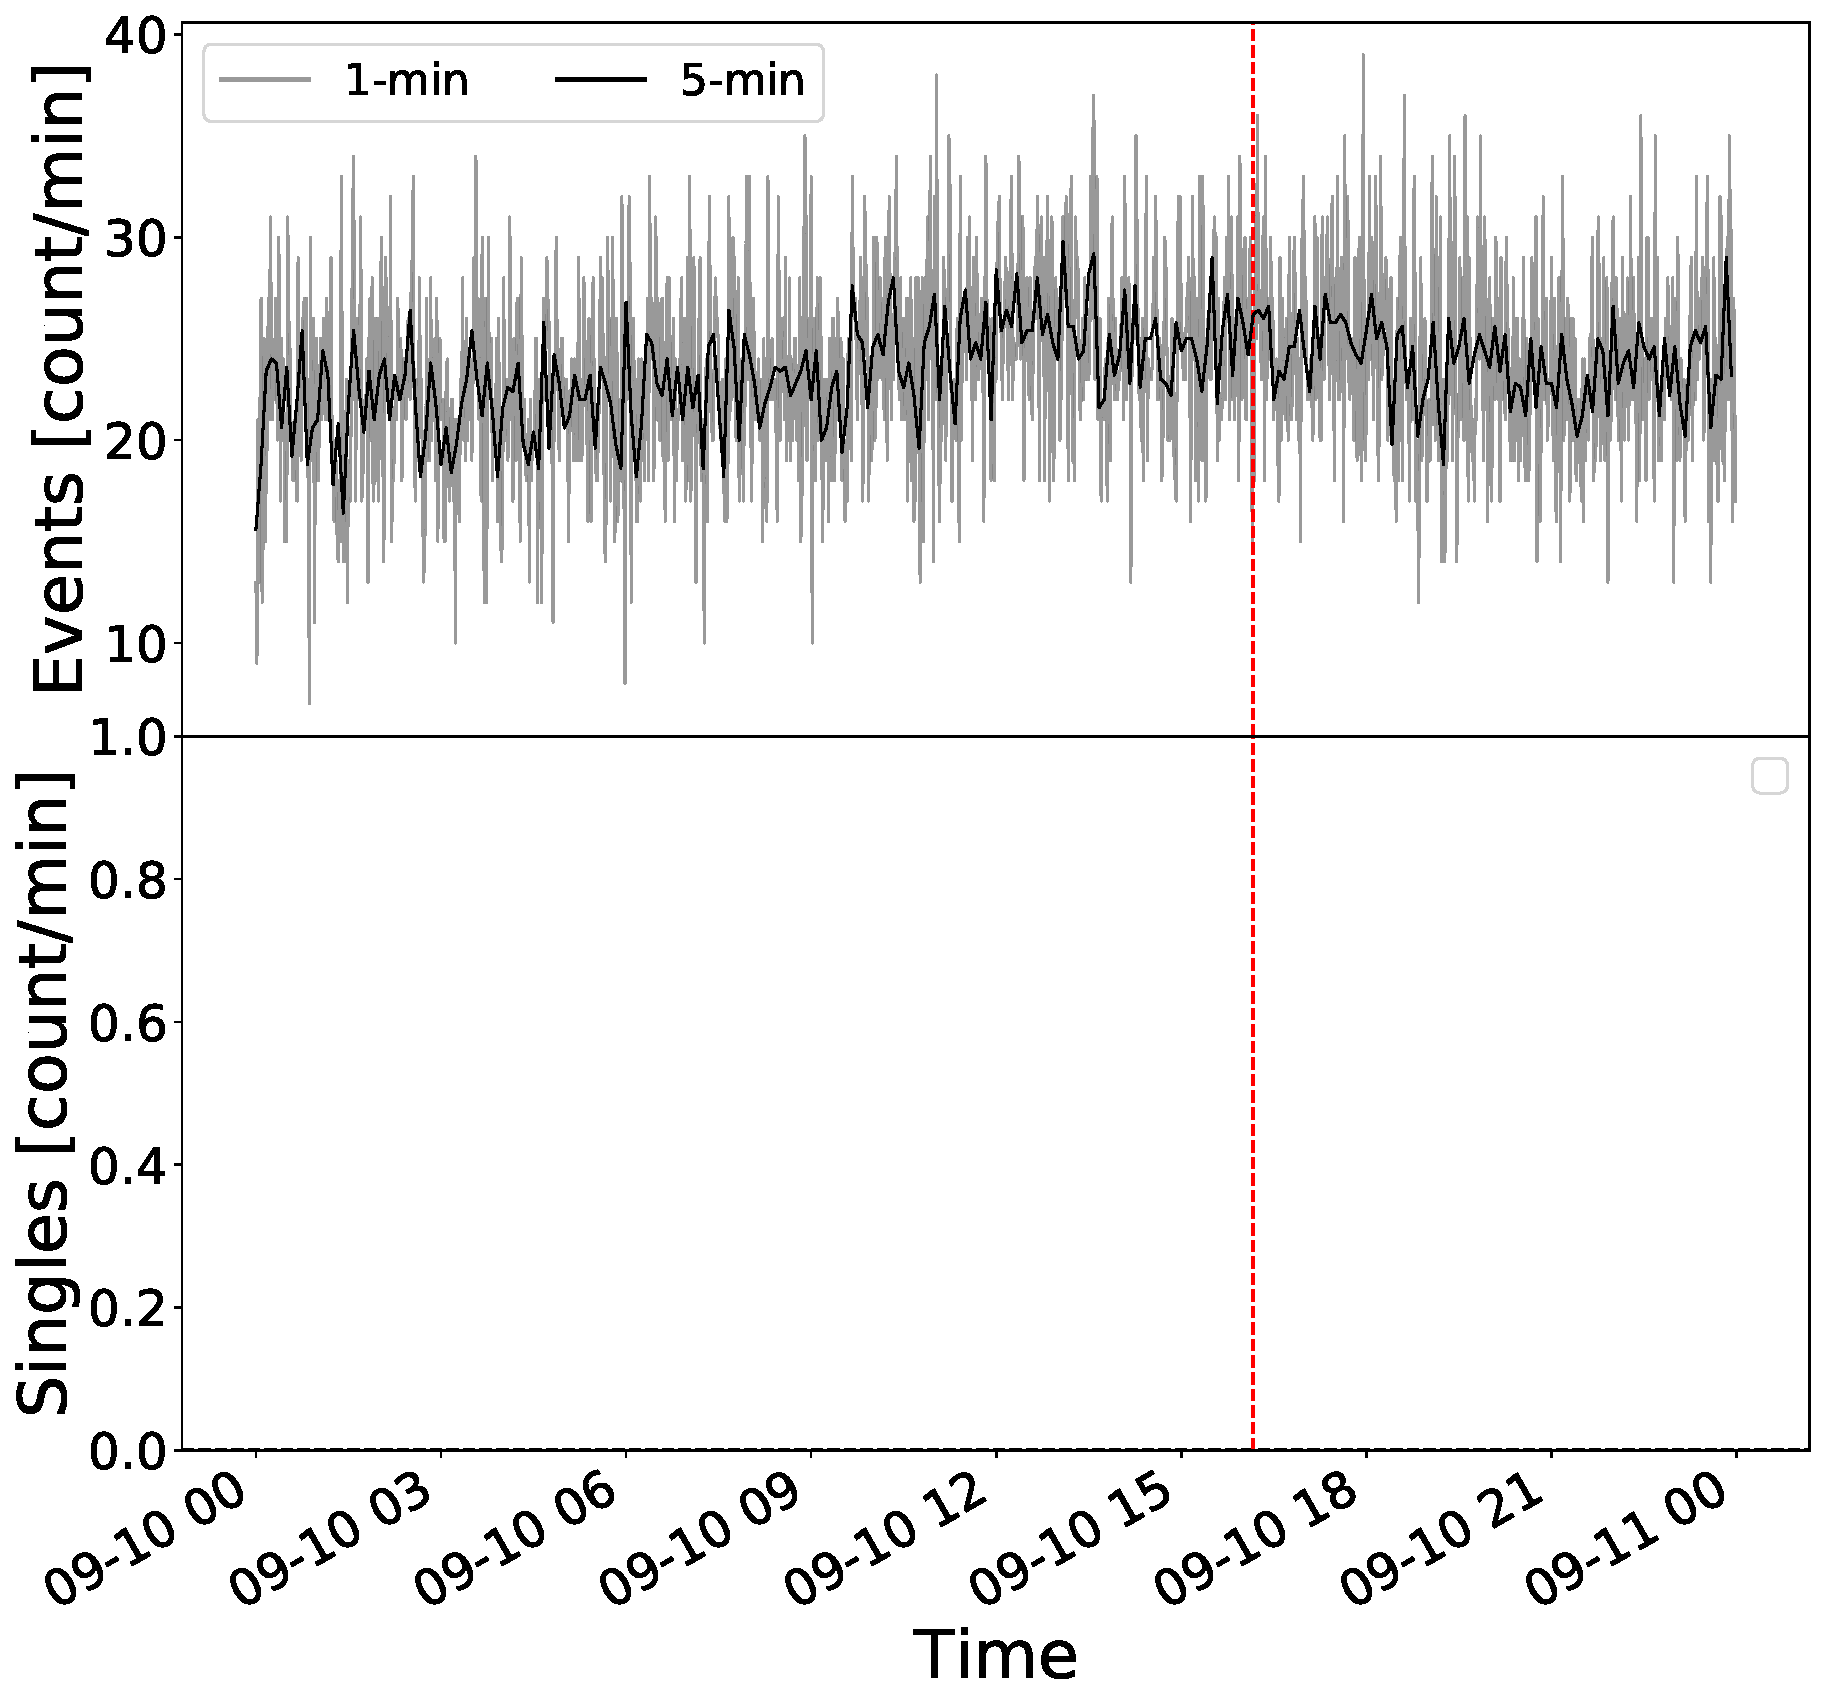
\includegraphics[width=0.48\columnwidth]{GLE72_14001.pdf}
		\label{fig:GLE72_14001}}
	
	\caption{HiSPARC data for 4 stations around the epoch of GLE 72 on 10/09/2017. The top panel of each subplot shows the 1-minute (grey) and 5-minute (black) averaged trigger events between detectors within the station, while the bottom panel shows the 1- and 5-minute averaged singles counts, mean-subtracted, for each individual detector (or signal channel, CH$n$) in the station. The vertical red, dashed line depicts the approximate onset time of the GLE. The units of time on the x-axis are, MM-DD HH.}
	\label{fig:GLE_72}
\end{figure}


We can see from Figures~\ref{fig:GLE_70},~\ref{fig:GLE_71}, and~\ref{fig:GLE_72} there are no clear and obvious signs of the \gls{gle} signals in the \gls{hisparc} observations, as was clear for those given in Fig.~\ref{fig:oulu_gles} for the Oulu \gls{nm} station, in Finland. This is the case for both the events data and the singles data.

There are some excursions from the mean count rate which make it difficult to determine variations from space weather events and other sources; this is significantly more prominent in the singles rates which are shown in the \gls{gle} 72 plots (Fig.~\ref{fig:GLE_72}) for stations 501, 203, and 8001. These excursions are the effect of atmospheric pressure and temperature on the muon count rates; in Section~\ref{sec:HS_standardisation} this is discussed further and the effect is accounted for. After its removal we then re-investigated the corrected data, which is discussed in Section~\ref{sec:HS_obs_Pcorr}. We also see the existence of a diurnal signal in Figure~\ref{fig:GLE71_8001}, with \gls{cr} count rates peaking at around midday. We expect a daily variation from a combination of the \gls{cr} anisotropy in the interplanetary space and the rotation of the Earth meaning detectors look in different directions over the course of a day. The diurnal variation is expected to have a magnitude of $<1\%$ \citep{mishra_study_2007, mishra_cosmic_2008, dubey_cosmic_2016, thomas_decadal_2017}, but here we see an increase of $\sim50-100\%$, which suggests there may be an additional factor causing the signal.

No clear \glspl{gle} have been observed in the \gls{hisparc} data. We believe this is due, in-part, to the rigidity cut-off of the \gls{hisparc} stations, as well as the different particle species observed by \gls{hisparc} compared to the \glspl{nm}. However, \citet{humble_j._e._detection_2012} state that \gls{nm} stations with cut-off rigidities up to $\sim 15$~GV observed the \gls{gle} in September 1989, indicating that \glspl{sep} up to at least $\sim 15$~GeV must have been present in the spectrum during that particularly large event. Therefore, the rigidity cut-off of the \gls{hisparc} stations is not necessarily the limiting factor. It is also possible that the \glspl{sep} which induced these \glspl{gle} were lower-energy \glspl{pcr} and therefore were insufficient to produce \glspl{eas} of muons; we know the \gls{hisparc} network is nominally used for observations of \glspl{uhecr} with energies several orders of magnitude larger.

\glspl{gle} are normally associated with \glspl{sep} with energies in the MeV to low-GeV regime; hence why \glspl{gle} are typically observed by \glspl{nm}. Only the most energetic events have been observed by \glspl{md} as they are more sensitive to the hard component of the \gls{pcr} spectrum \citep{augusto_signals_2016}. Observations of \glspl{gle} with \gls{hisparc} will therefore only be linked with the the maximum energy release during solar flares, and often this is very short and still the \glspl{sep} are of insufficient energy to be detected by \glspl{md} \citep{mccracken_high-energy_2012, augusto_signals_2016}. 

To further understand the impact of \gls{sep} energies on the \gls{hisparc} observations, in Section~\ref{sec:CORSIKA} we used air shower simulations to investigate the \gls{cr} spectrum at quiet times and during \glspl{gle}. %We do also note that the atmospheric effects in the raw do not help our ability to observe the space weather and these effects were later removed (see Section~\ref{sec:HS_P_corr}).


%%%%%%%%%%%%%%%%%%%%%%%%%%%%%%%%%%%%%%%%%%%%%%%%%%%%%%%%%%%%%%%%%%%%%
\subsection{Observations of Forbush Decreases}


The search for evidence of \glspl{fd} within the \gls{hisparc} data was conducted for the \glspl{fd} highlighted in Table~\ref{tab:space_weather_events}. Figures~\ref{fig:FD_201203}, ~\ref{fig:FD_201207}, and ~\ref{fig:FD_201412} show the \gls{hisparc} observations around the epochs of the first four \glspl{fd} listed in Table~\ref{tab:space_weather_events}. Each of the plots shows only observations using the \gls{hisparc} events data (i.e. coincidences between the detectors of a station), as singles data were not available at those epochs (see Fig.~\ref{fig:HS_data_availability}).

\begin{figure}[ht!]
	\centering
	\subfloat[HS 501 (Nikhef)]{
		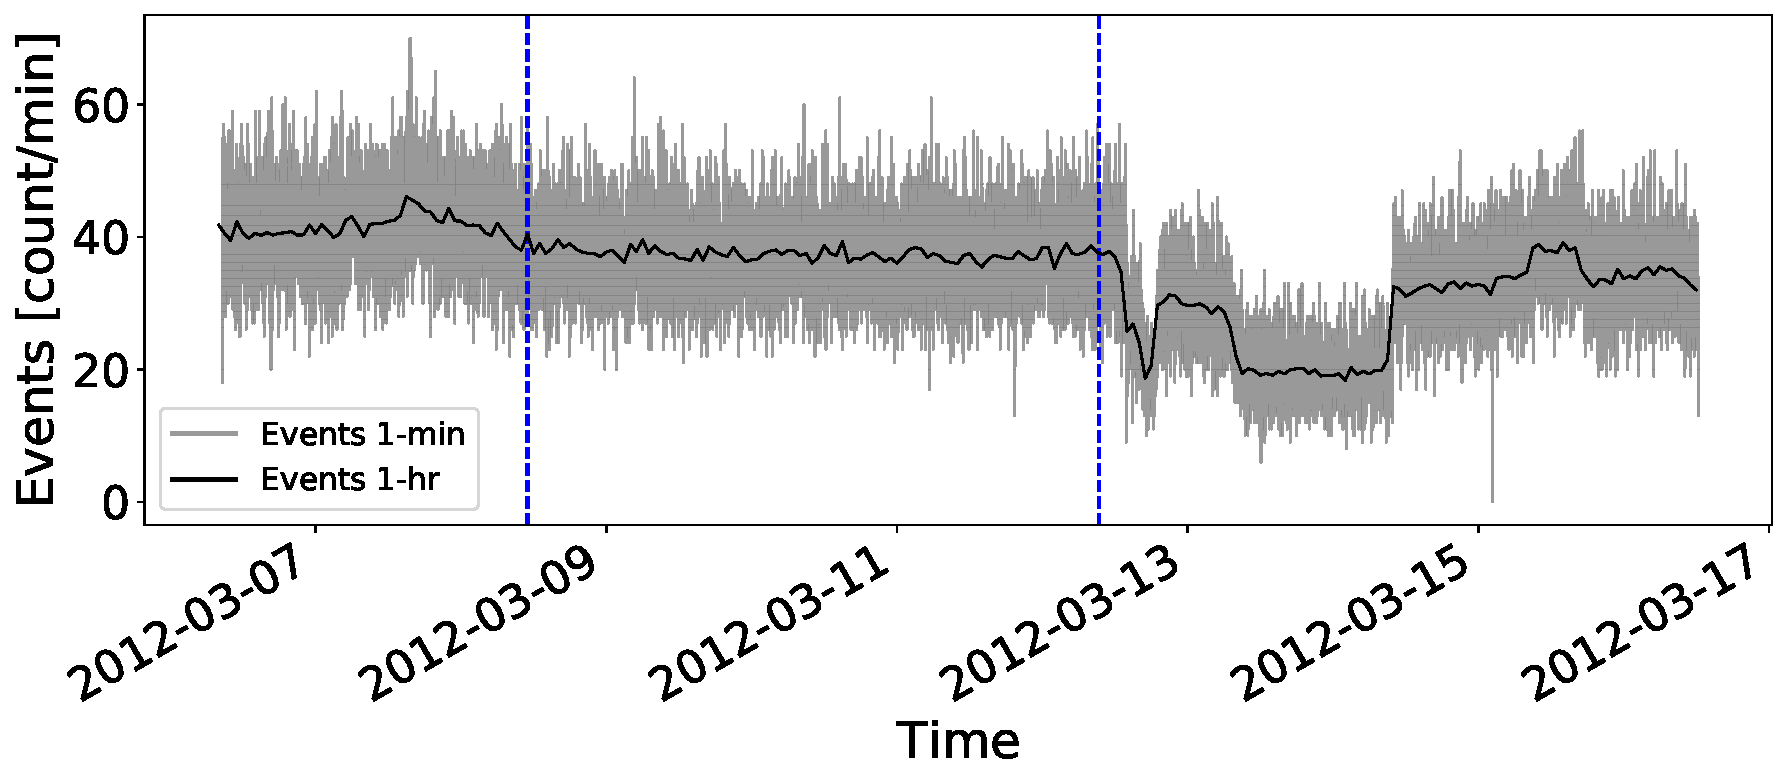
\includegraphics[width=0.48\columnwidth]{FD_201203_501.pdf}
		\label{fig:FD_201203_501}}
	%\qquad
	\subfloat[HS 8001 (Eindhoven)]{
		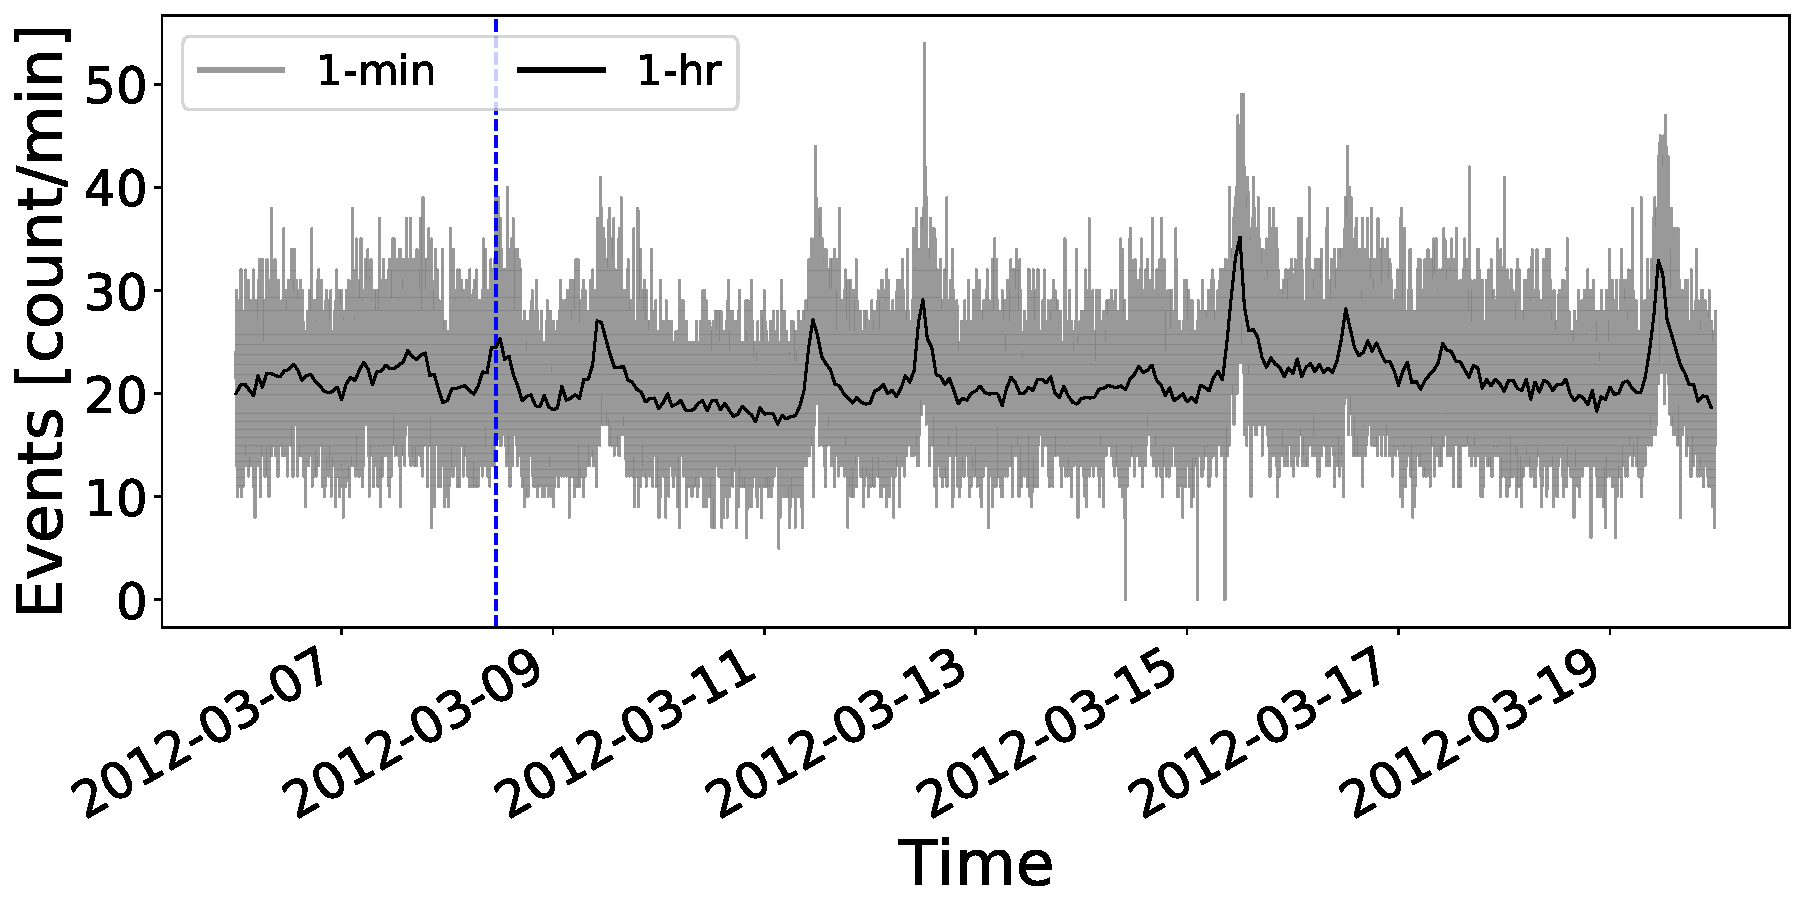
\includegraphics[width=0.48\columnwidth]{FD_201203_8001.pdf}
		\label{fig:FD_201203_8001}}
	
	\caption{HiSPARC data for stations 501 and 8001 around the epoch of the FDs in March 2012. The plot shows the minute-averaged (grey) and hourly-averaged (black) trigger events between detectors within the station. The vertical blue-dashed lines show the approximate onset-time of the FDs. The units of time on the x-axis are, YYYY-MM-DD.}
	\label{fig:FD_201203}
\end{figure}

\begin{figure}[ht!]
	\centering
	\subfloat[HS 501 (Nikhef)]{
		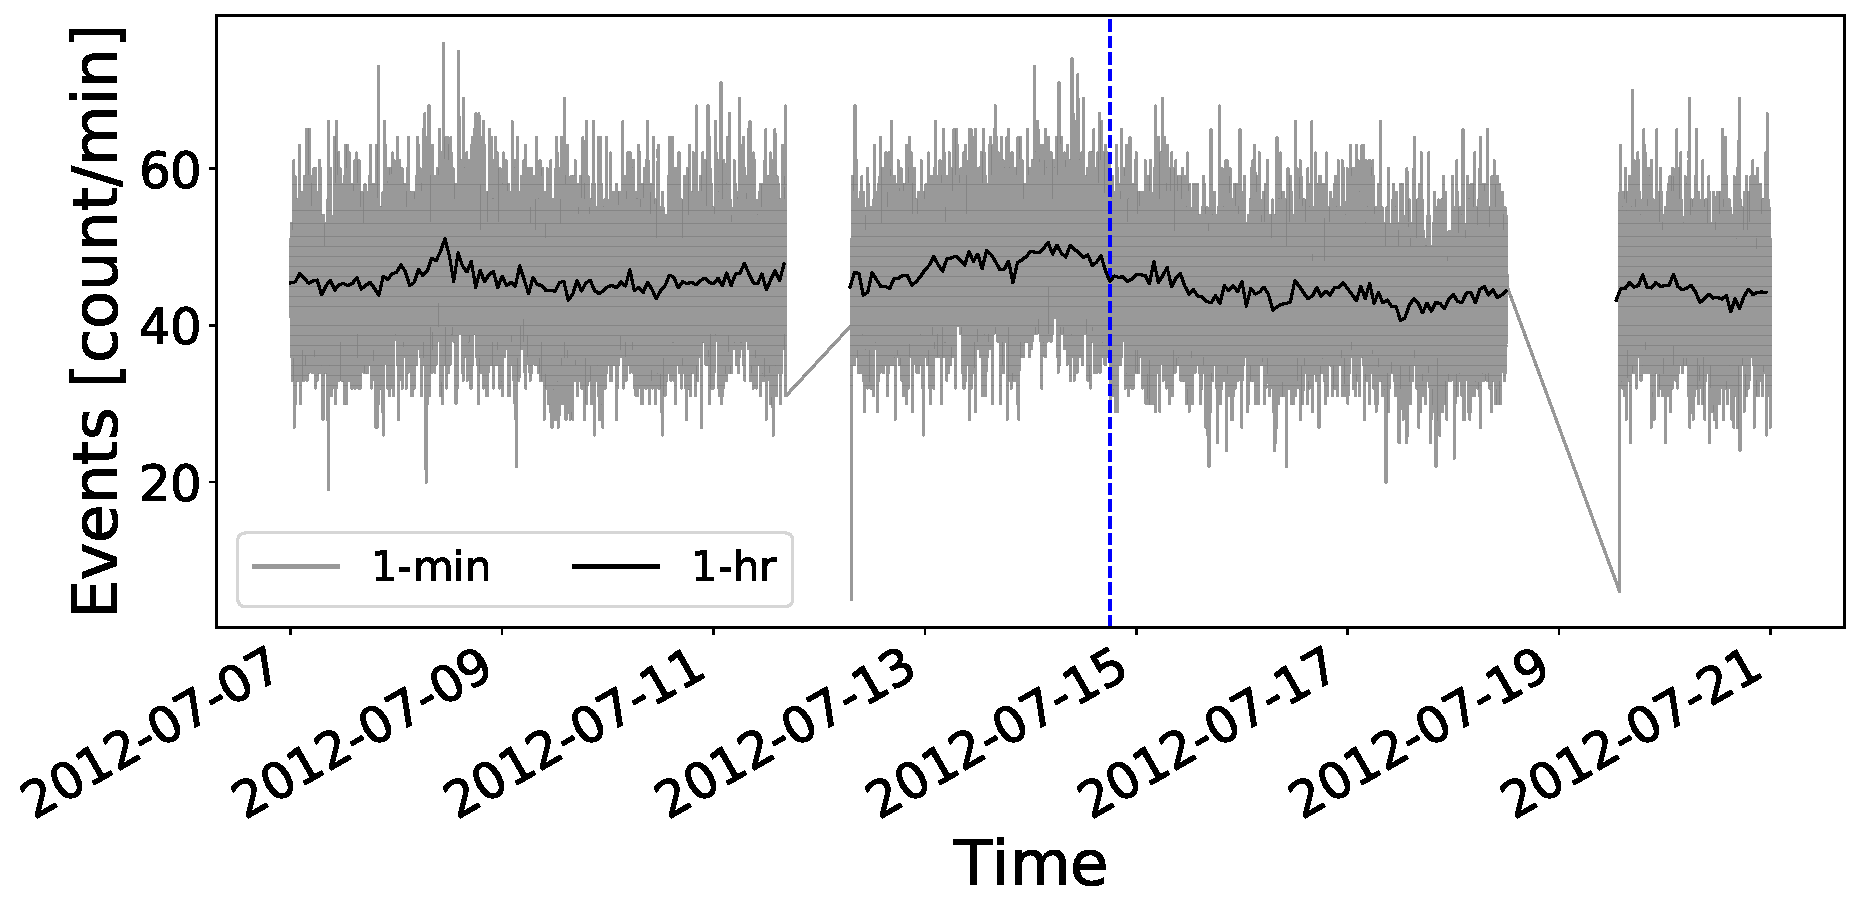
\includegraphics[width=0.48\columnwidth]{FD_201207_501.pdf}
		\label{fig:FD_201207_501}}
	%\qquad
	\subfloat[HS 8001 (Eindhoven)]{
		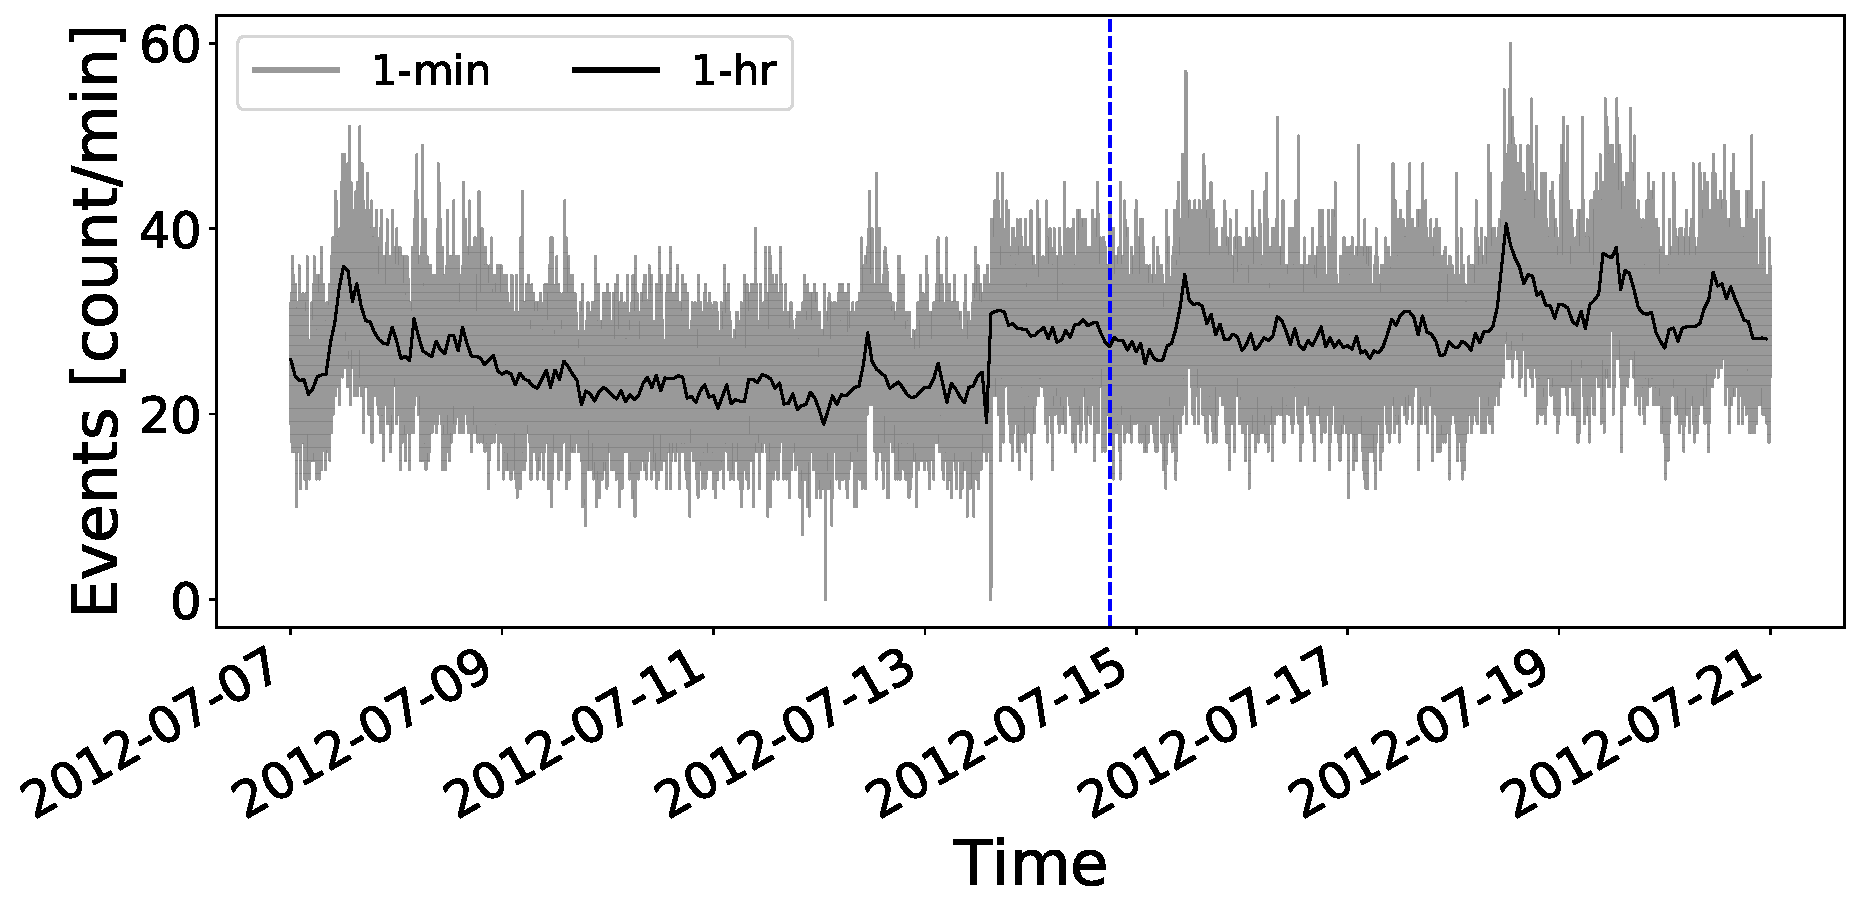
\includegraphics[width=0.48\columnwidth]{FD_201207_8001.pdf}
		\label{fig:FD_201207_8001}}
	
	\caption{HiSPARC data for stations 501 and 8001 around the epoch of the FD in July 2012. The plot shows the minute-averaged (grey) and hourly-averaged (black) trigger events between detectors within the station. The vertical blue-dashed line shows the approximate onset-time of the FD. The units of time on the x-axis are, YYYY-MM-DD.}
	\label{fig:FD_201207}
\end{figure}

\begin{figure}[ht!]
	\centering
	\subfloat[HS 501 (Nikhef)]{
		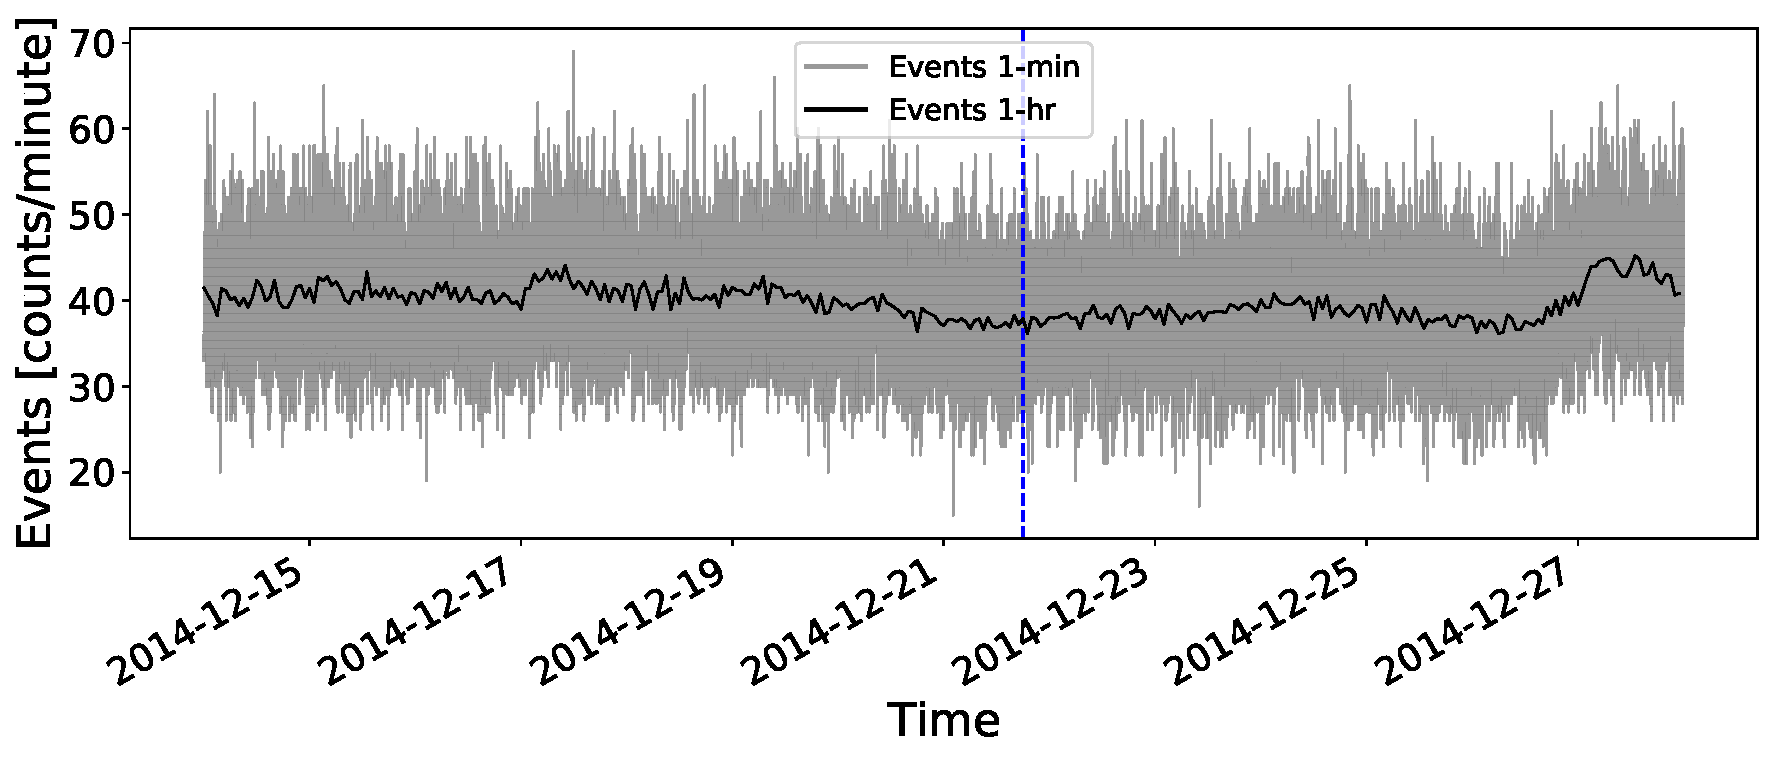
\includegraphics[width=0.48\columnwidth]{FD_201412_501.pdf}
		\label{fig:FD_201412_501}}
	%\qquad
	\subfloat[HS 203 (College Hageveld)]{
		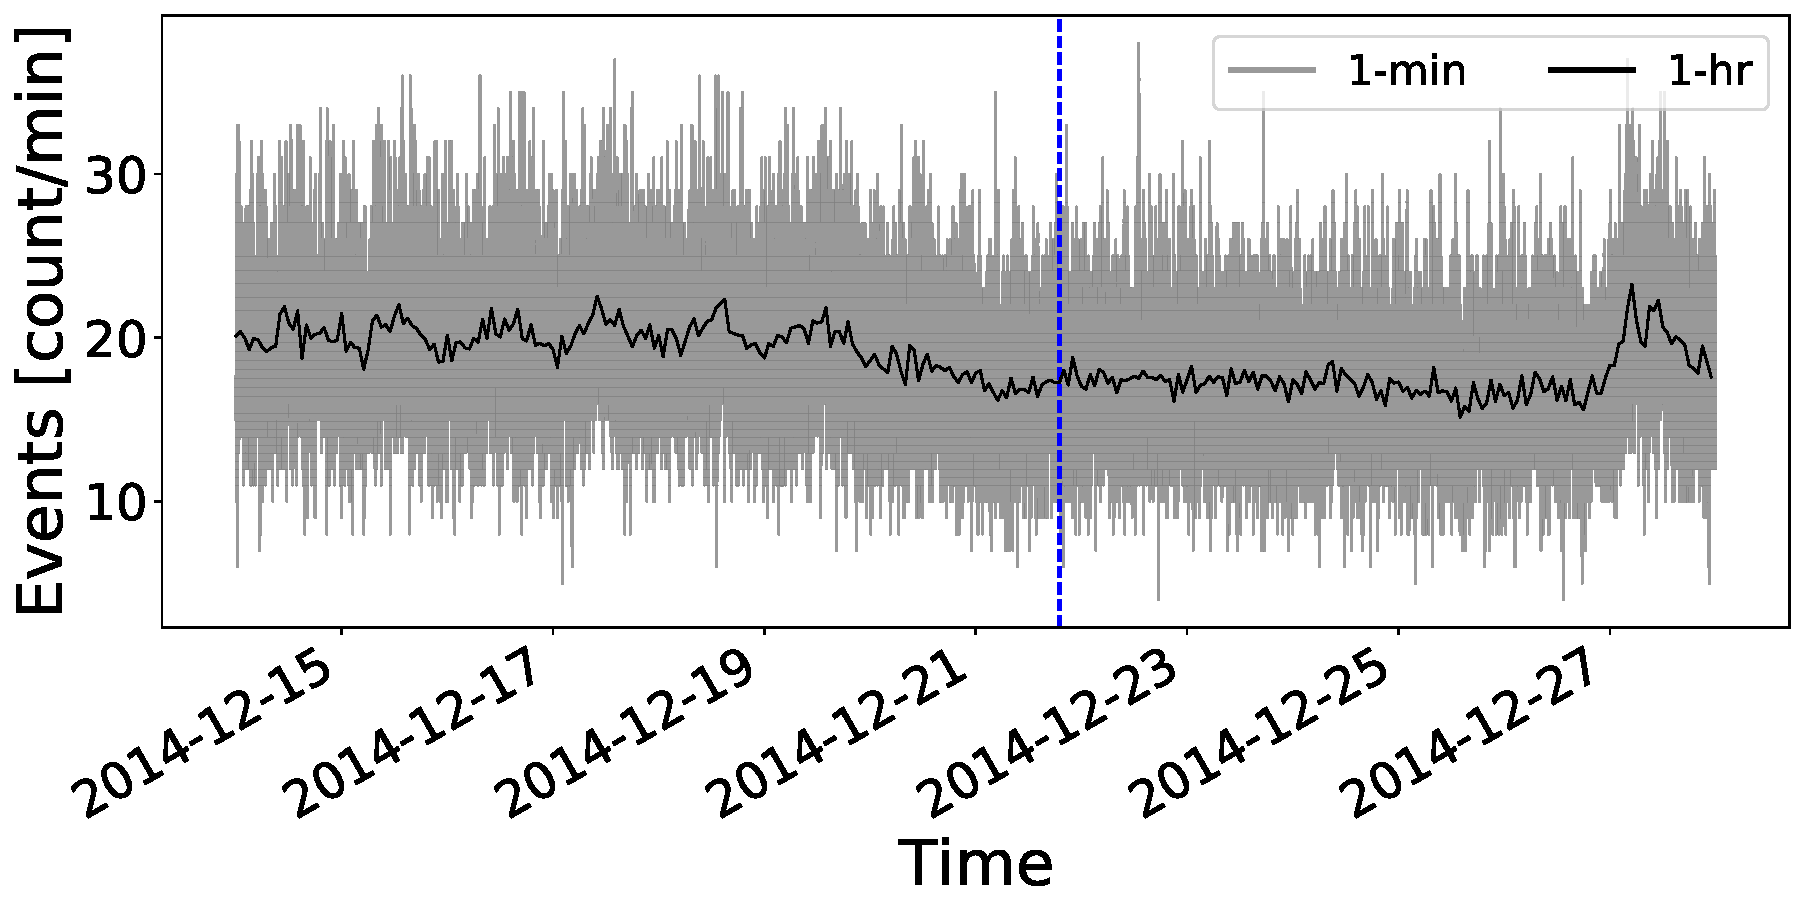
\includegraphics[width=0.48\columnwidth]{FD_201412_203.pdf}
		\label{fig:FD_201412_203}} \\
	
	\qquad
	
	\subfloat[HS 3001 (Leiden)]{
		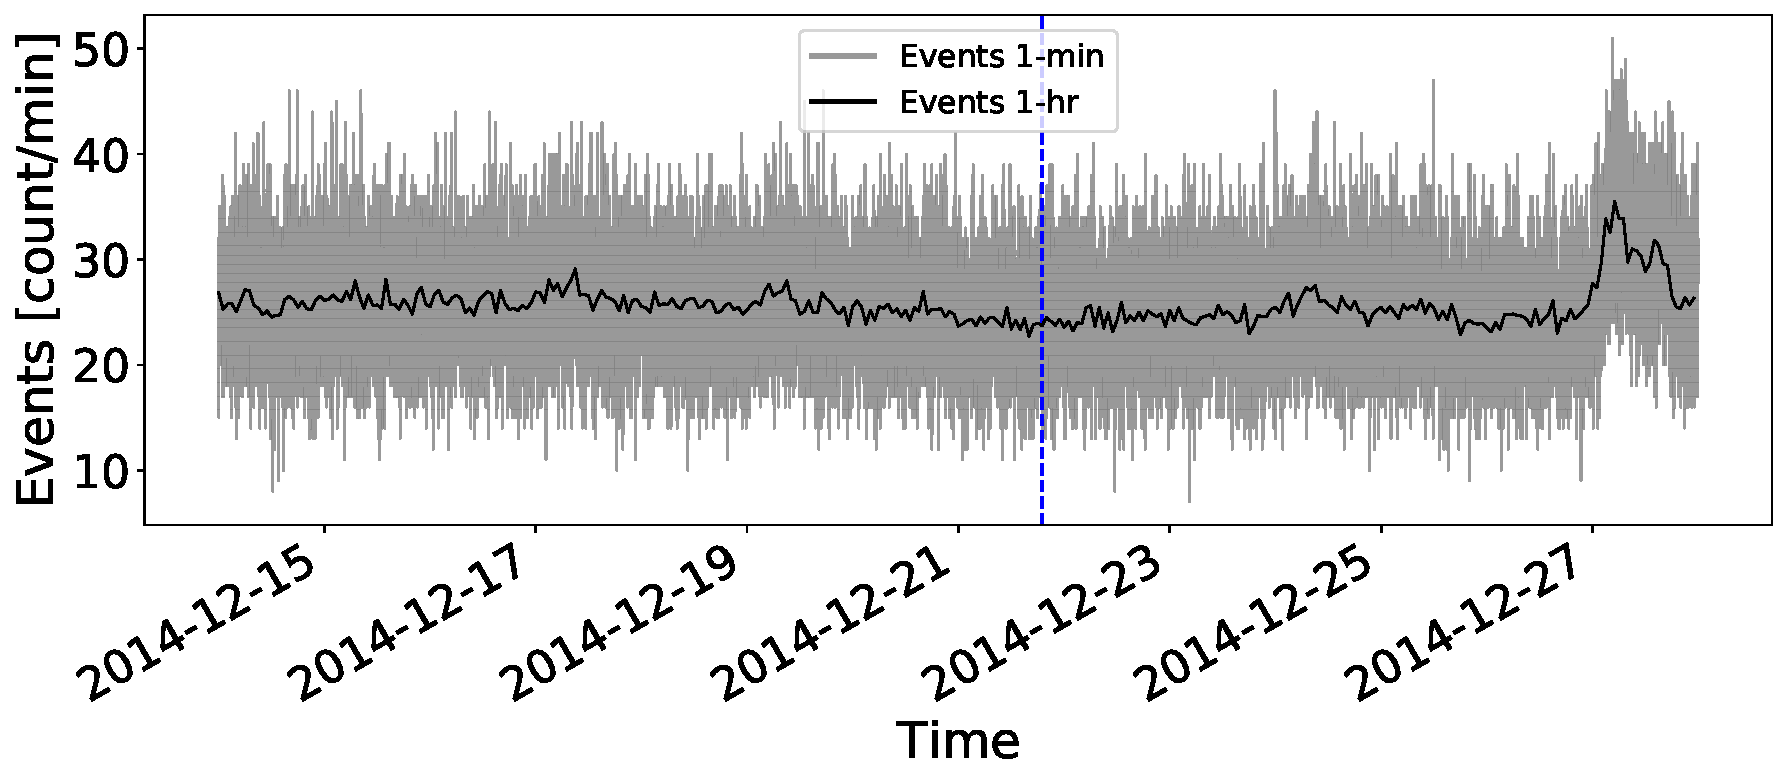
\includegraphics[width=0.48\columnwidth]{FD_201412_3001.pdf}
		\label{fig:FD_201412_3001}}
	%\qquad
	\subfloat[HS 14001 (Birmingham University)]{
		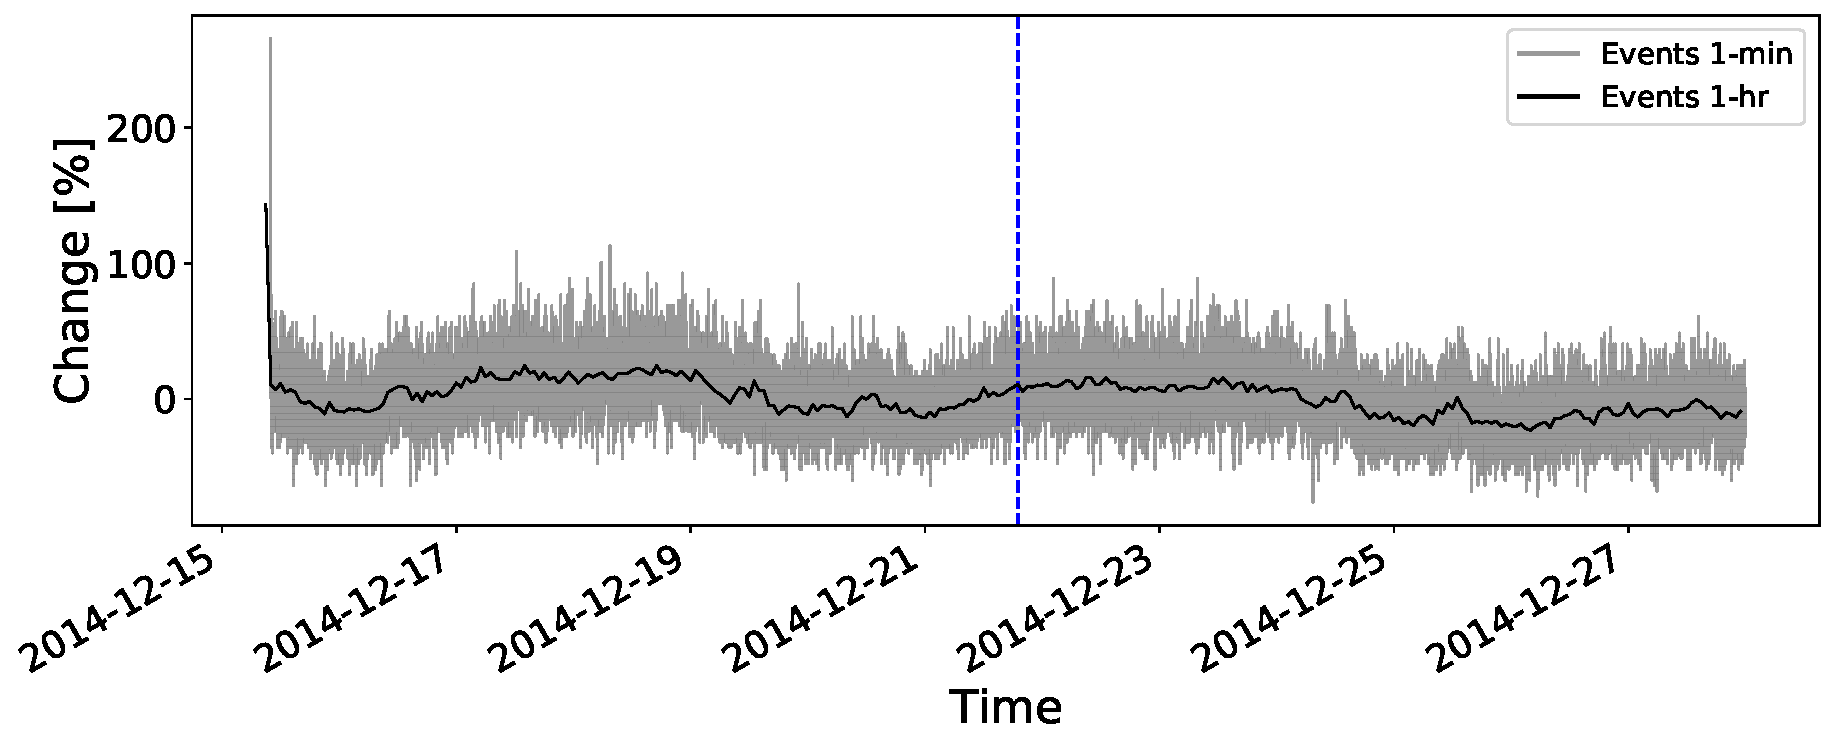
\includegraphics[width=0.48\columnwidth]{FD_201412_14001.pdf}
		\label{fig:FD_201412_14001}}
	
	\caption{HiSPARC data for four stations around the epoch of the FD in December 2014. The plot shows the minute-averaged (grey) and hourly-averaged (black) trigger events between detectors within the station. The vertical blue-dashed line shows the approximate onset-time of the FD. The units of time on the x-axis are, YYYY-MM-DD.}
	\label{fig:FD_201412}
\end{figure}


We can see from the plots that there were no clear signs of the \gls{fd} signals in the \gls{hisparc} data shown here. We observed a set of significant decreases in the muon count rate in station 501 after the second \gls{fd} in March 2012 (see Figure~\ref{fig:FD_201203_501}); however, it is unclear whether this was a consequence of the \gls{fd} or other hardware reasons, as the \gls{fd} was not observed in the other \gls{hisparc} stations. The shape of the \gls{fd} in the \gls{nm} data shows a sudden decrease and a smooth recovery within two days, but the shape of the \gls{hisparc} observations traces a more complex evolution, which suggests that the cause is not the \gls{fd}, but rather a result of hardware.

As we saw with the earlier investigation into \glspl{gle}, we again see excursions from the mean count rate which vary over longer time scales. This is due to metrological variations in the atmosphere. In Section~\ref{sec:HS_standardisation} this is discussed further and the effect is accounted for.

In addition, it is quite clear from Figure~\ref{fig:FD_201203_8001} and Figure~\ref{fig:FD_201207_8001} that station 8001 (Eindhoven) displays a semi-persistent diurnal variation in the count rate. We typically expect a diurnal variation of $<1\%$ \citep{mishra_study_2007, mishra_cosmic_2008, dubey_cosmic_2016, thomas_decadal_2017}, but here we see an increase of $\sim 100\%$, which again suggests there may be an additional factor.%know that daily variation is a combination of the \gls{cr} anisotropy in the interplanetary space and a consequence of the rotation of the Earth meaning detectors look in different directions over the course of a day; however, we


\begin{figure}[htb!]
	\centering
	\subfloat[HS 501 (Nikhef)]{
		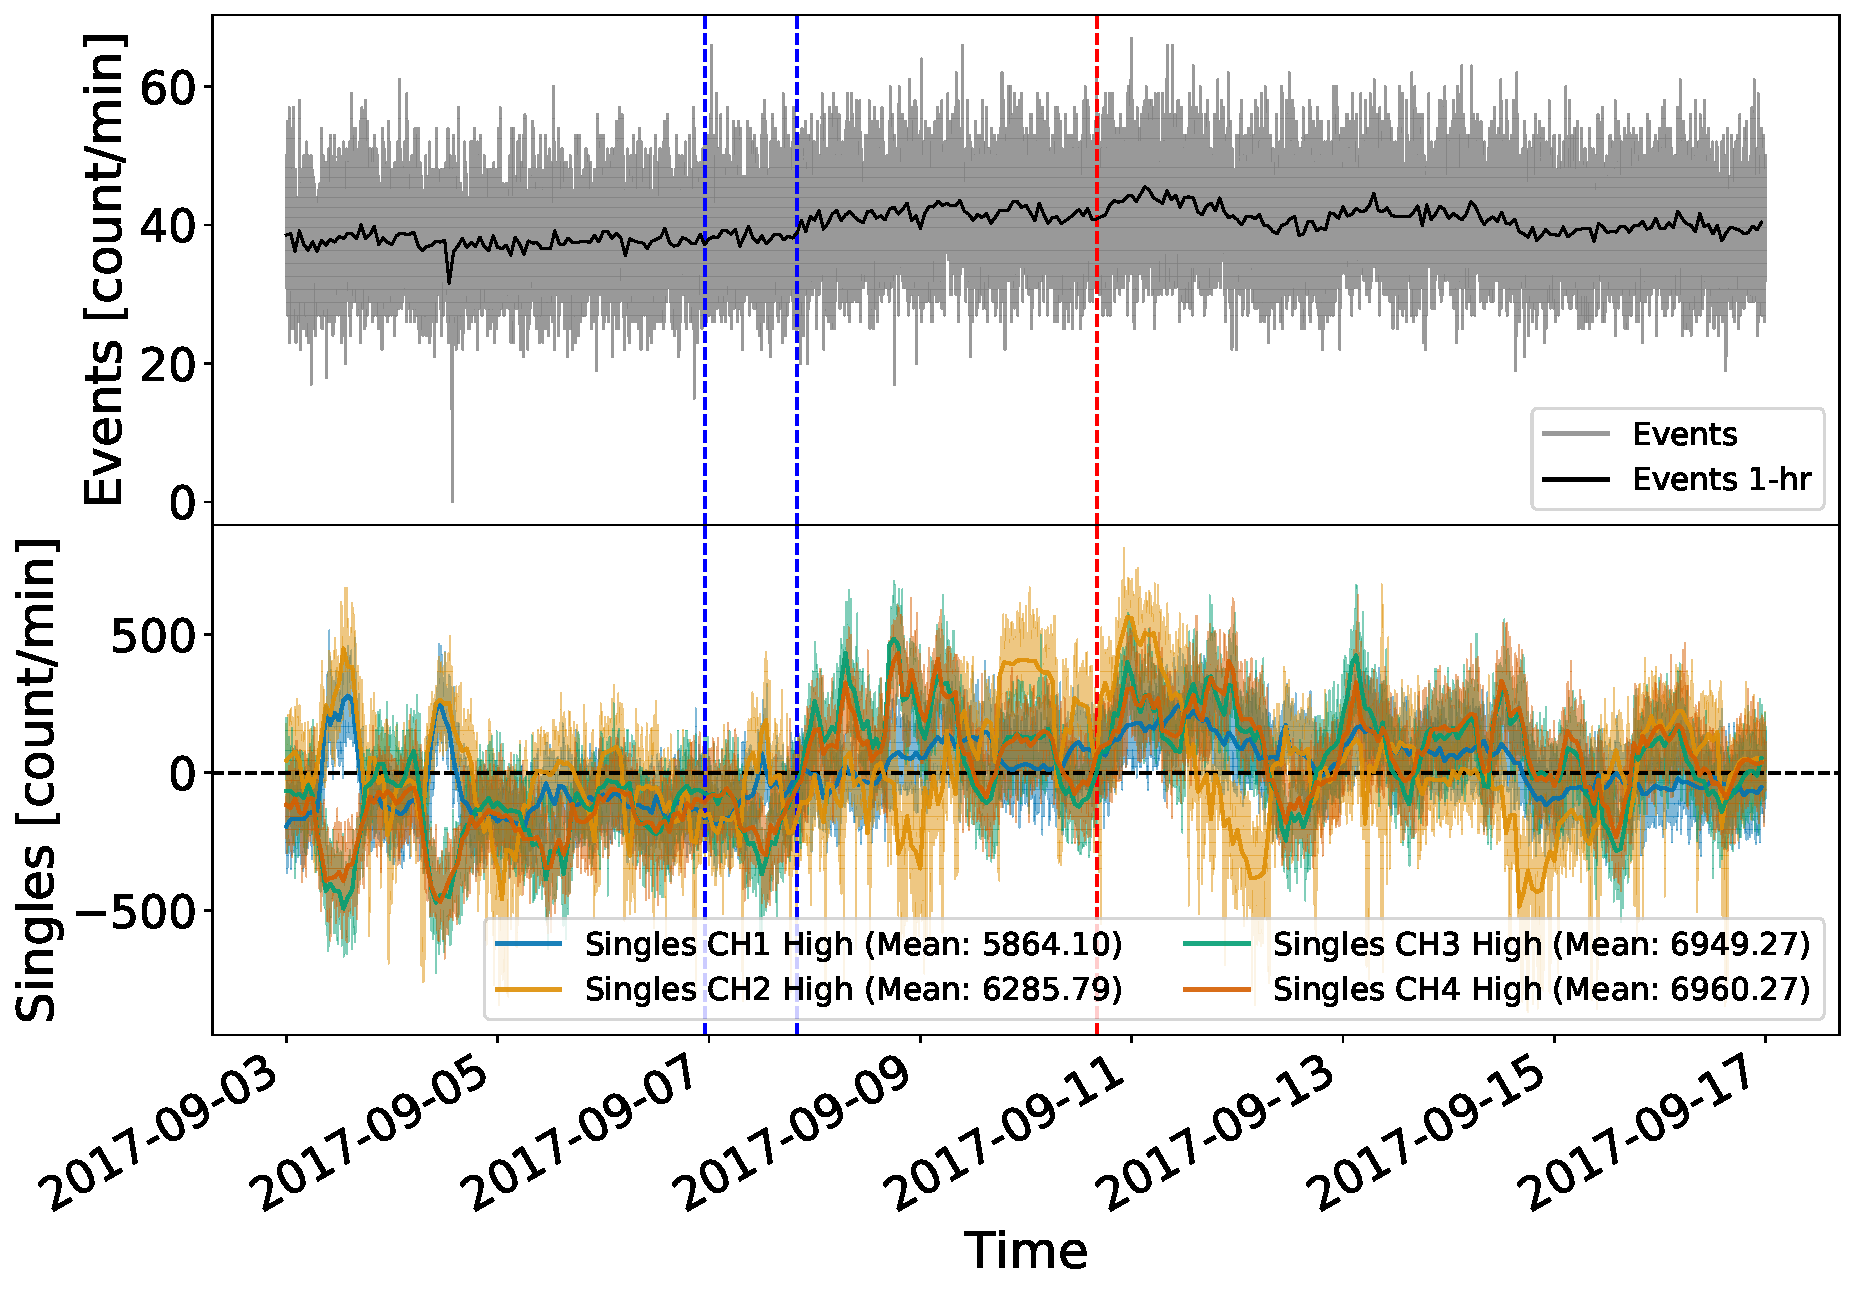
\includegraphics[width=0.48\columnwidth]{FD_GLE72_501.pdf}
		\label{fig:FD_GLE72_501}}
	%\qquad
	\subfloat[HS 203 (College Hageveld)]{
		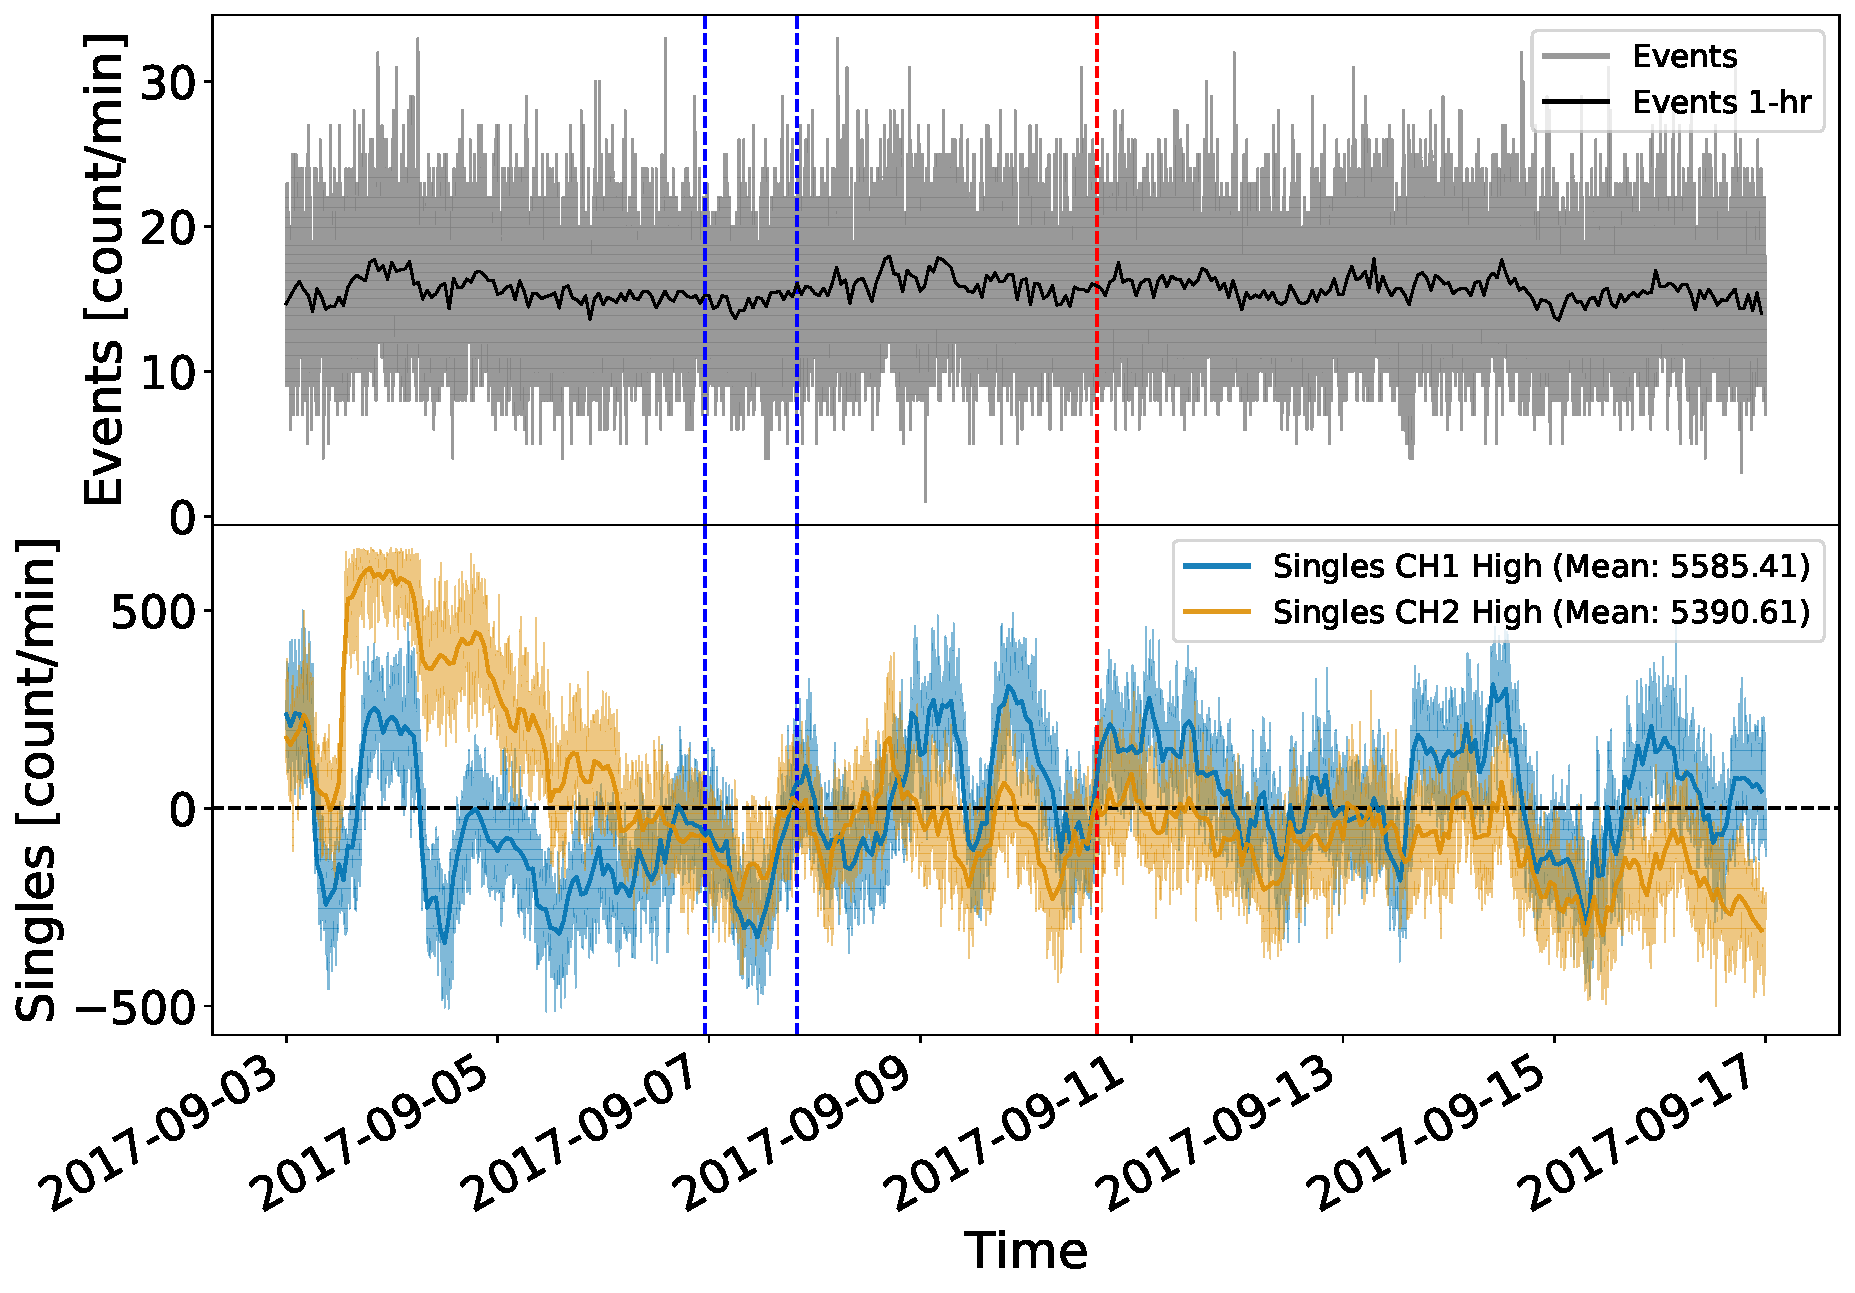
\includegraphics[width=0.48\columnwidth]{FD_GLE72_203.pdf}
		\label{fig:FD_GLE72_203}} \\
	
	\qquad
	
	\subfloat[HS 8001 (Eindhoven)]{
		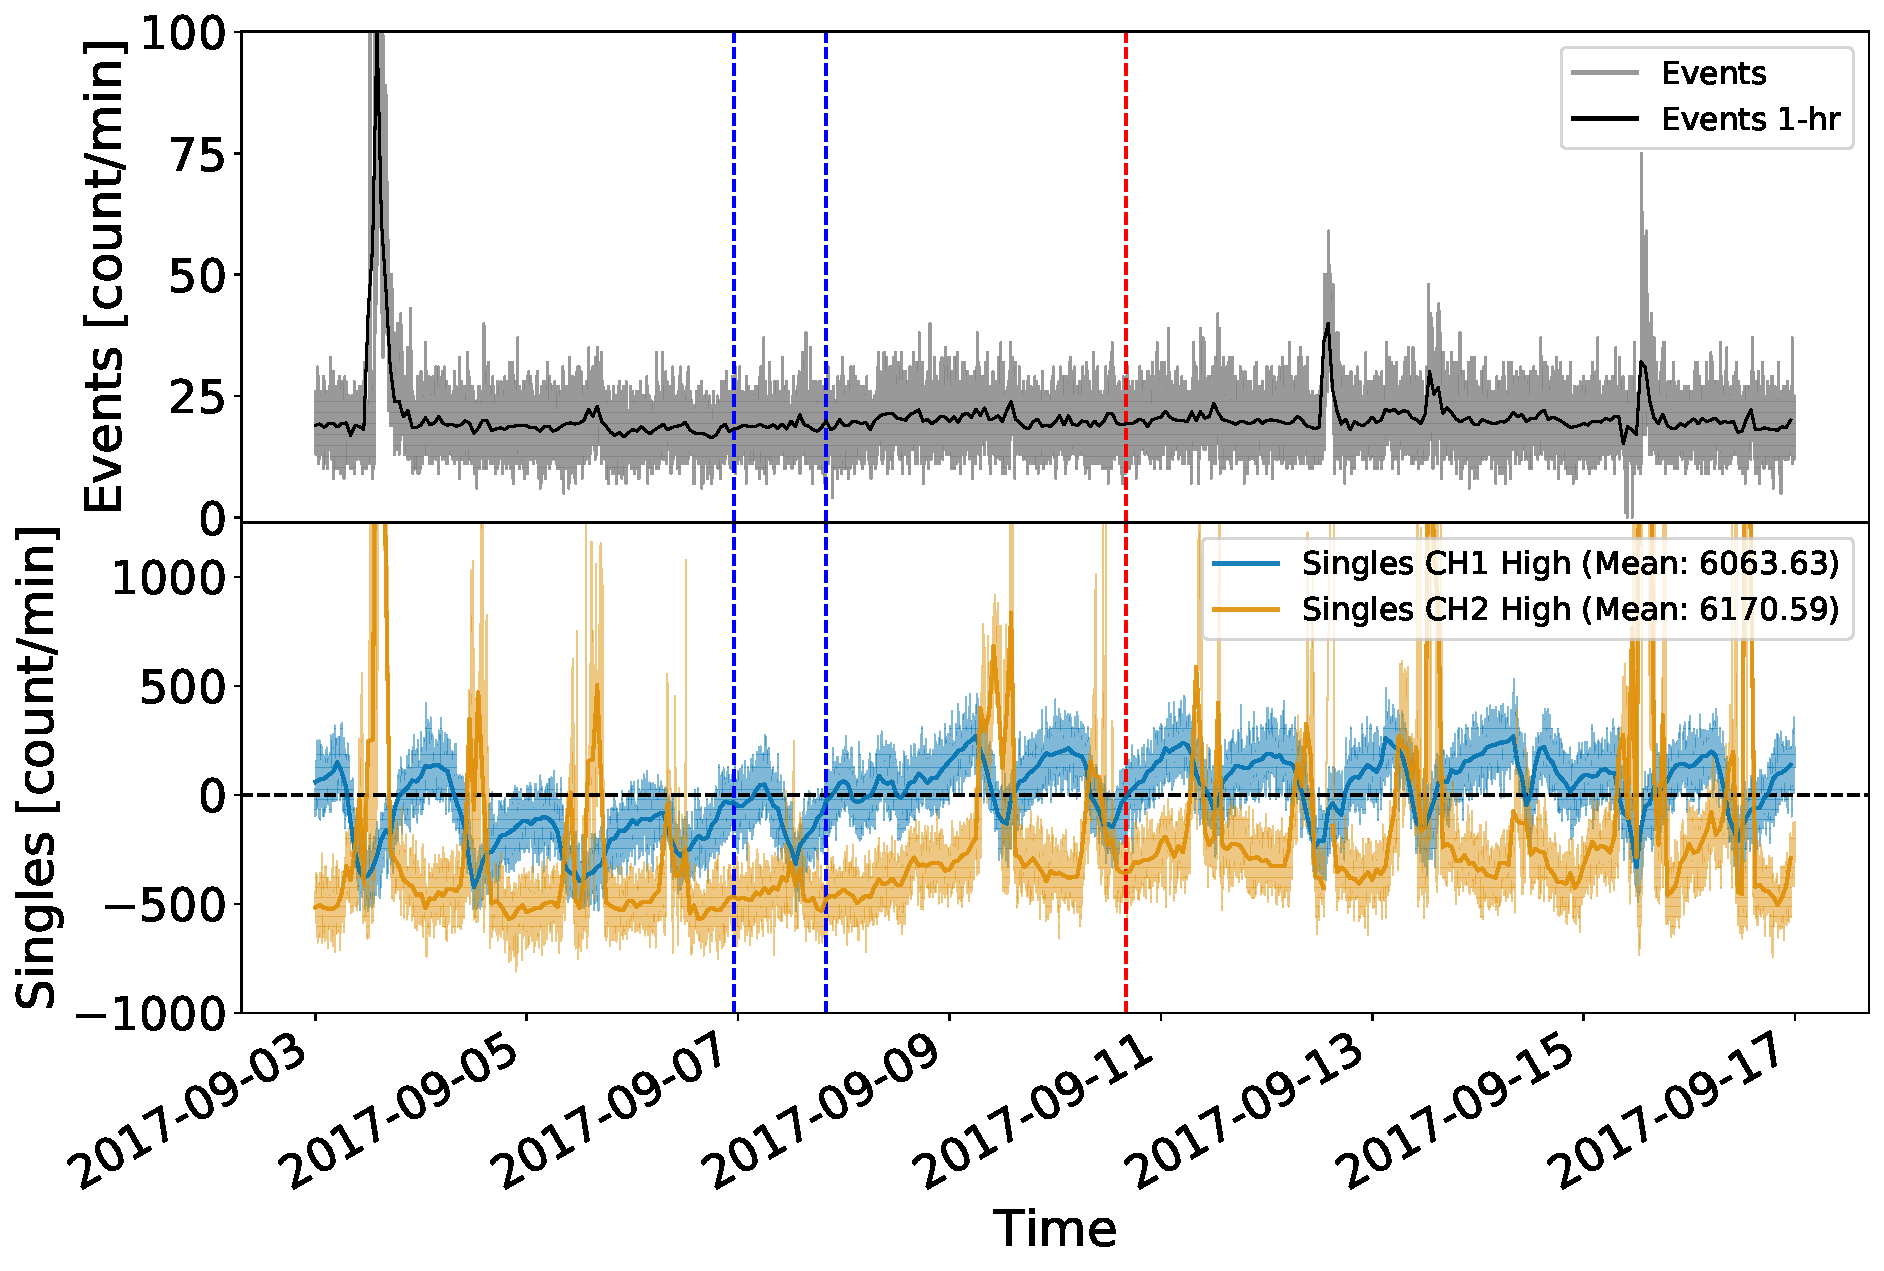
\includegraphics[width=0.48\columnwidth]{FD_GLE72_8001.pdf}
		\label{fig:FD_GLE72_8001}}
	%\qquad
	\subfloat[HS 14001 (Birmingham University)]{
		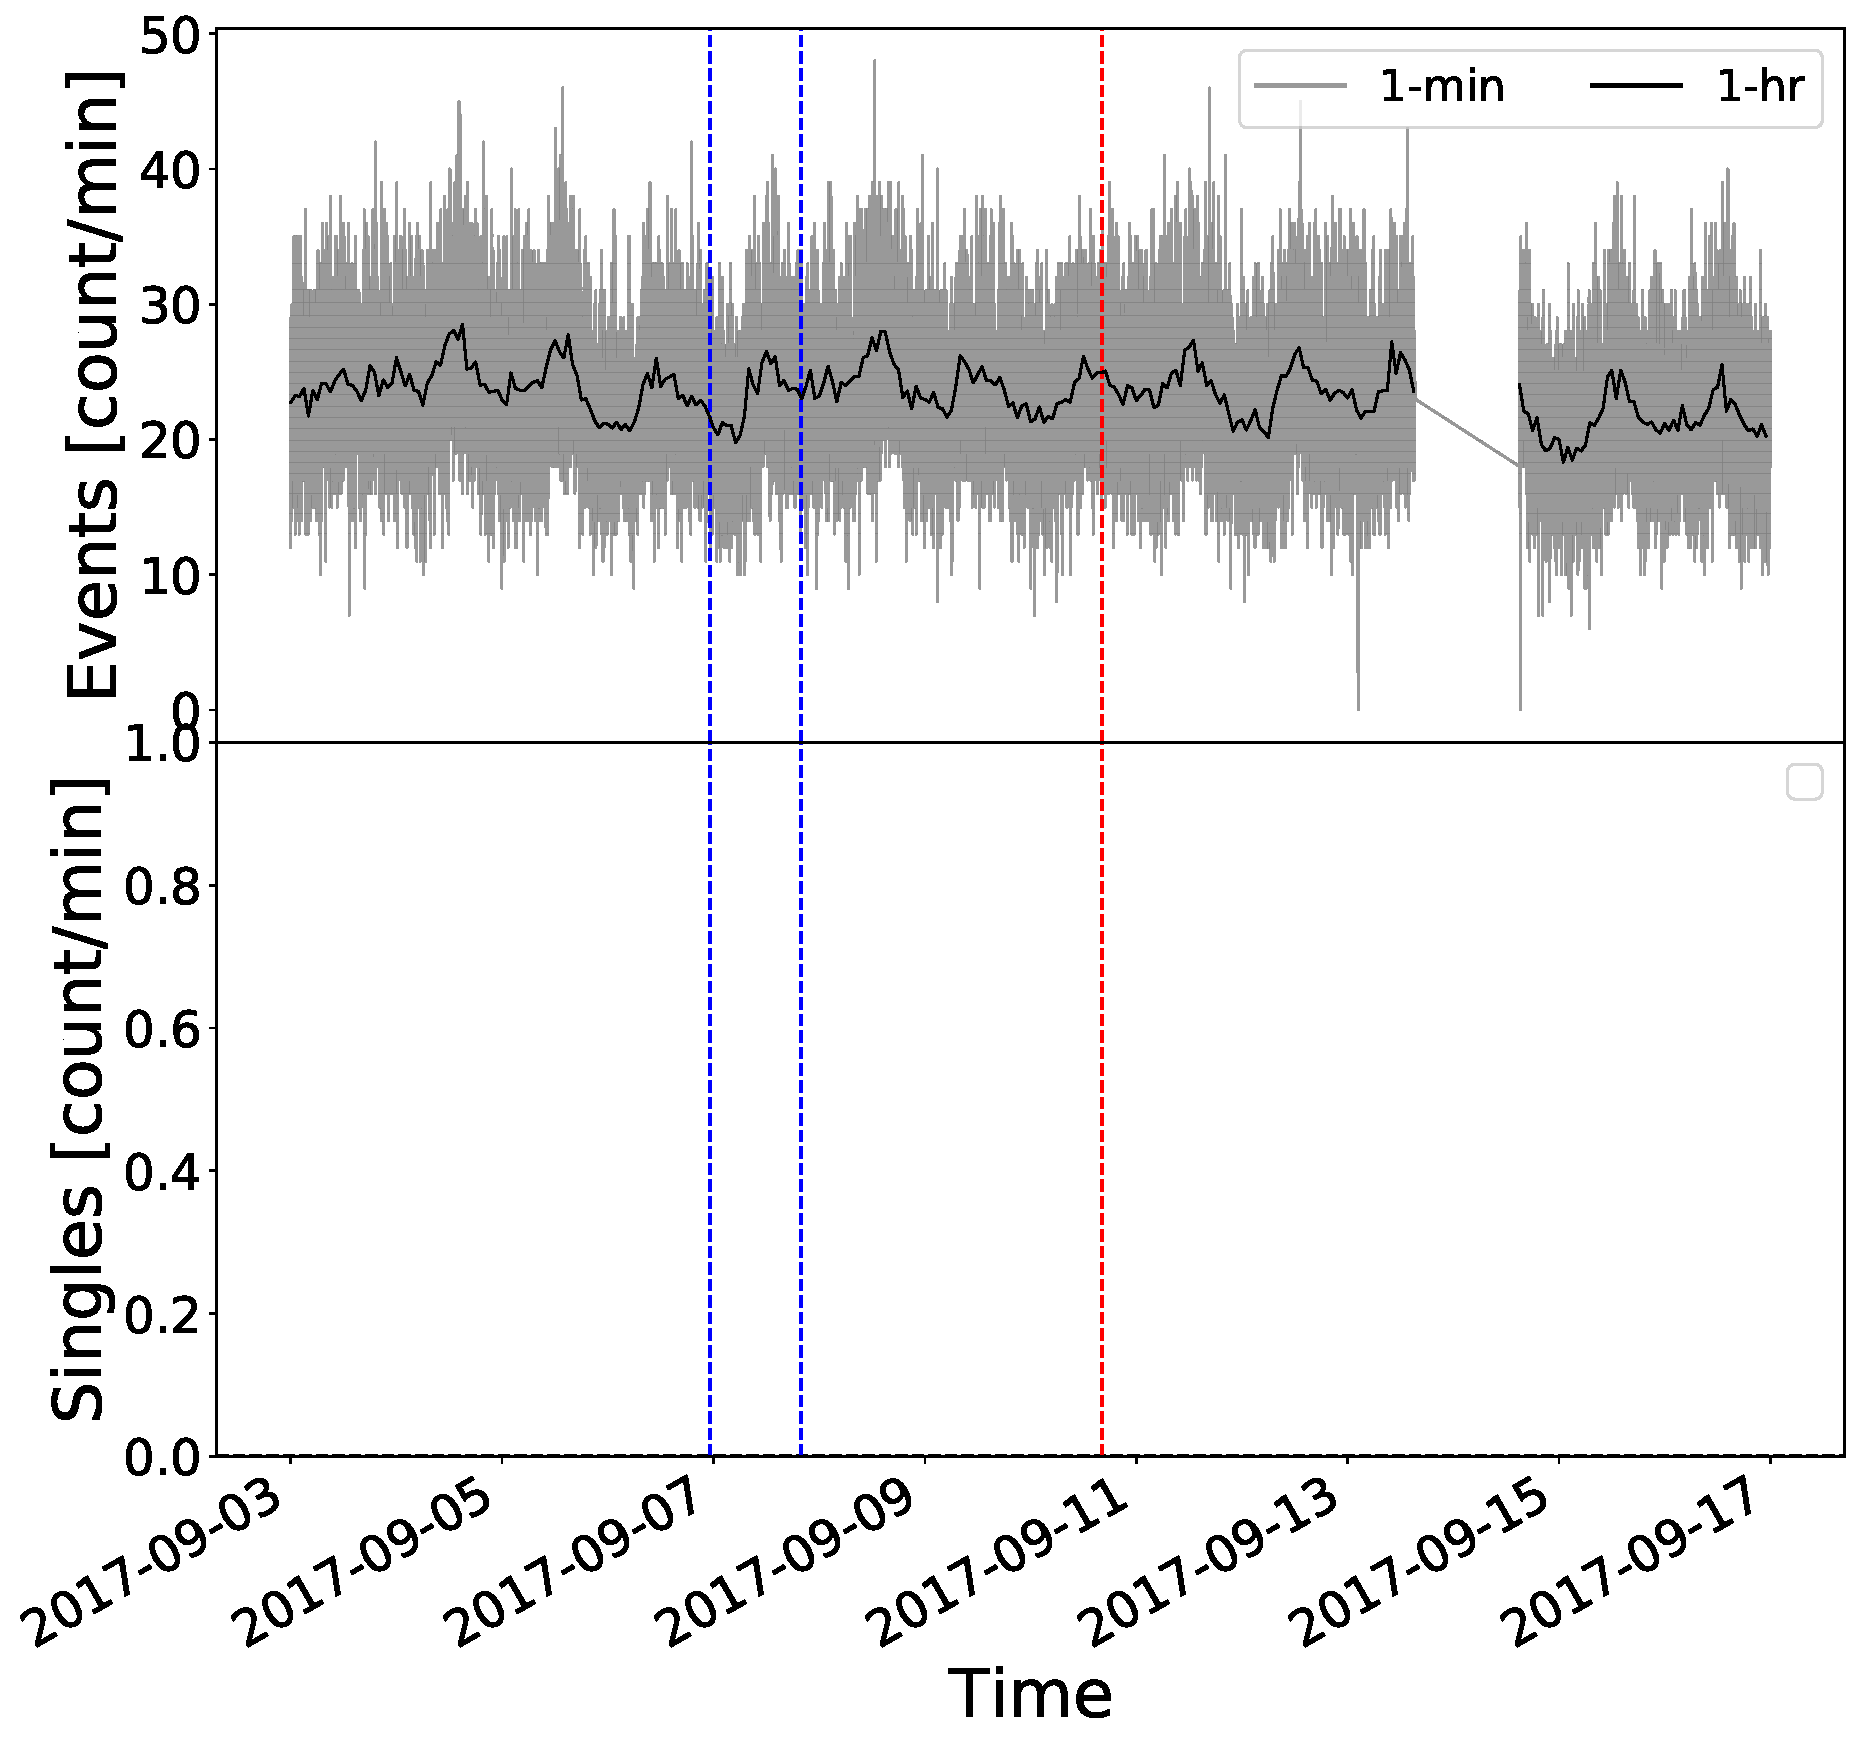
\includegraphics[width=0.48\columnwidth]{FD_GLE72_14001.pdf}
		\label{fig:FD_GLE72_14001}}
	
	\caption{HiSPARC data for four stations around the epoch in which there were two FDs close to the onset of GLE 72. The top panel of each subplot shows the minute-averaged (grey) and hourly-averaged (back) trigger events between detectors within the station, while the bottom panel shows the minute- and hourly-averaged singles counts, mean-subtracted, for each individual detector (or channel, CH$n$) in the station. The vertical blue-dashed lines show the approximate onset-times of the two FDs observed around this epoch and the red-dashed line depicts the approximate onset time of the GLE. The units of time on the x-axis are, YYYY-MM-DD.}
	\label{fig:FD_GLE72}
\end{figure}


For the final two \glspl{fd} listed in Table~\ref{tab:space_weather_events}, the plot of the \gls{hisparc} observations is shown in Figure~\ref{fig:FD_GLE72}. Plotted are the \gls{hisparc} events data; however, where possible, we also show the singles rates from each of the individual detectors in a station, when available. Furthermore, as these \glspl{fd} were precursory to \gls{gle} 72, we also marked on the epoch of the \gls{gle} for completeness.



As with the other \gls{fd} epochs, we again do not observe any clear signs of the \gls{fd} signals in either the events nor singles data. In each of the three stations for which there were singles data, we observed a semi-persistent diurnal signal. This was also seen in the events data for station 14001. In the singles data we see a strong diurnal variation of up to $\sim 100\%$ (see channel 2 in Fig.~\ref{fig:FD_GLE72_8001}). As previously discussed, we expect a diurnal variation of $< 1\%$, increasing around local midday \citep{mishra_study_2007, mishra_cosmic_2008, dubey_cosmic_2016, thomas_decadal_2017}; however, in Figure~\ref{fig:FD_GLE72_8001} not only do we see a stronger variation, we also see that the two detectors are anti-correlated, suggested that this signal is a manifestation of thermally induced noise in each detector.


%Furthermore, we again observed a slow variation in the count rate which is suspected to be due to atmospheric pressure and is discussed in Section~\ref{sec:HS_P_corr}.

We conclude that no clear signature of \glspl{fd} has been observed in the \gls{hisparc} data. We again believe this could be linked to the rigidity cut-off of the \gls{hisparc} stations, but also it is possible that the reason originates in the lower sensitivity to lower rigidity \glspl{pcr} of \glspl{md} compared to \glspl{nm}. We also note that the atmospheric effects in the raw data limit our ability to observe the space weather effects, therefore in the next section we remove these effects to standardise the \gls{hisparc} data. 


%\clearpage
%%%%%%%%%%%%%%%%%%%%%%%%%%%%%%%%%%%%%%%%%%%%%%%%%%%%%%%%%%%%%%%%%%%%%
%%%%%%%%%%%%%%%%%%%%%%%%%%%%%%%%%%%%%%%%%%%%%%%%%%%%%%%%%%%%%%%%%%%%%

\section{Atmospheric Corrections of HiSPARC Data}\label{sec:HS_standardisation}

%%%%%%%%%%%%%%%%%%%%%%%%%%%%%%%%%%%%%%%%%%%%%%%%%%%%%%%%%%%%%%%%%%%%%
\subsection{Motivation}

It is well known that observations made by ground-based \gls{cr} detectors are susceptible to atmospheric conditions \citep{dorman_theory_2004,dorman_cosmic_2010,berkova_temperature_2011,de_mendonca_analysis_2013,paschalis_online_2013}. As we have seen in the plots shown in Section~\ref{sec:HS_obs}, there exist excursions in the data whose origins are from atmospheric variations. This sensitivity makes it difficult to differentiate between variations due space weather events and those due to Earth's atmospheric conditions, therefore it was necessary to correct for these effects in the data.

%- HiSPARC stations are individually managed and guidelines aren't stringent
%- Variability between stations exists and also apparently between detectors within a station (i.e. see singles during \gls{gle} 72)


%%%%%%%%%%%%%%%%%%%%%%%%%%%%%%%%%%%%%%%%%%%%%%%%%%%%%%%%%%%%%%%%%%%%%
\subsection{Barometric Correction}\label{sec:HS_P_corr}


Atmospheric pressure affects the \gls{cr} path length due to the expansion and contraction of the atmosphere with varying pressure \citep{dorman_theory_1972, paschalis_online_2013}; hence the \gls{cr} counts are observed to be negatively correlated to atmospheric pressure as shown for both \glspl{nm} and \glspl{md} in Figure~\ref{fig:CR_V_P}. 

A correction for this barometric effect is routinely applied as part of the data calibration for all \gls{nm} stations within the \gls{nmdb} and an online barometric coefficient tool\footnote{\url{http://cosray.phys.uoa.gr/index.php/data/nm-barometric-coefficient}} is available for \glspl{nm}, which allows users to perform the barometric correction for a given station over a user-defined epoch \citep{paschalis_online_2013}. There is no such process routinely applied in the \gls{hisparc} data pipeline.


\begin{figure}[ht!]
	\centering
	\subfloat[NM Station]{
		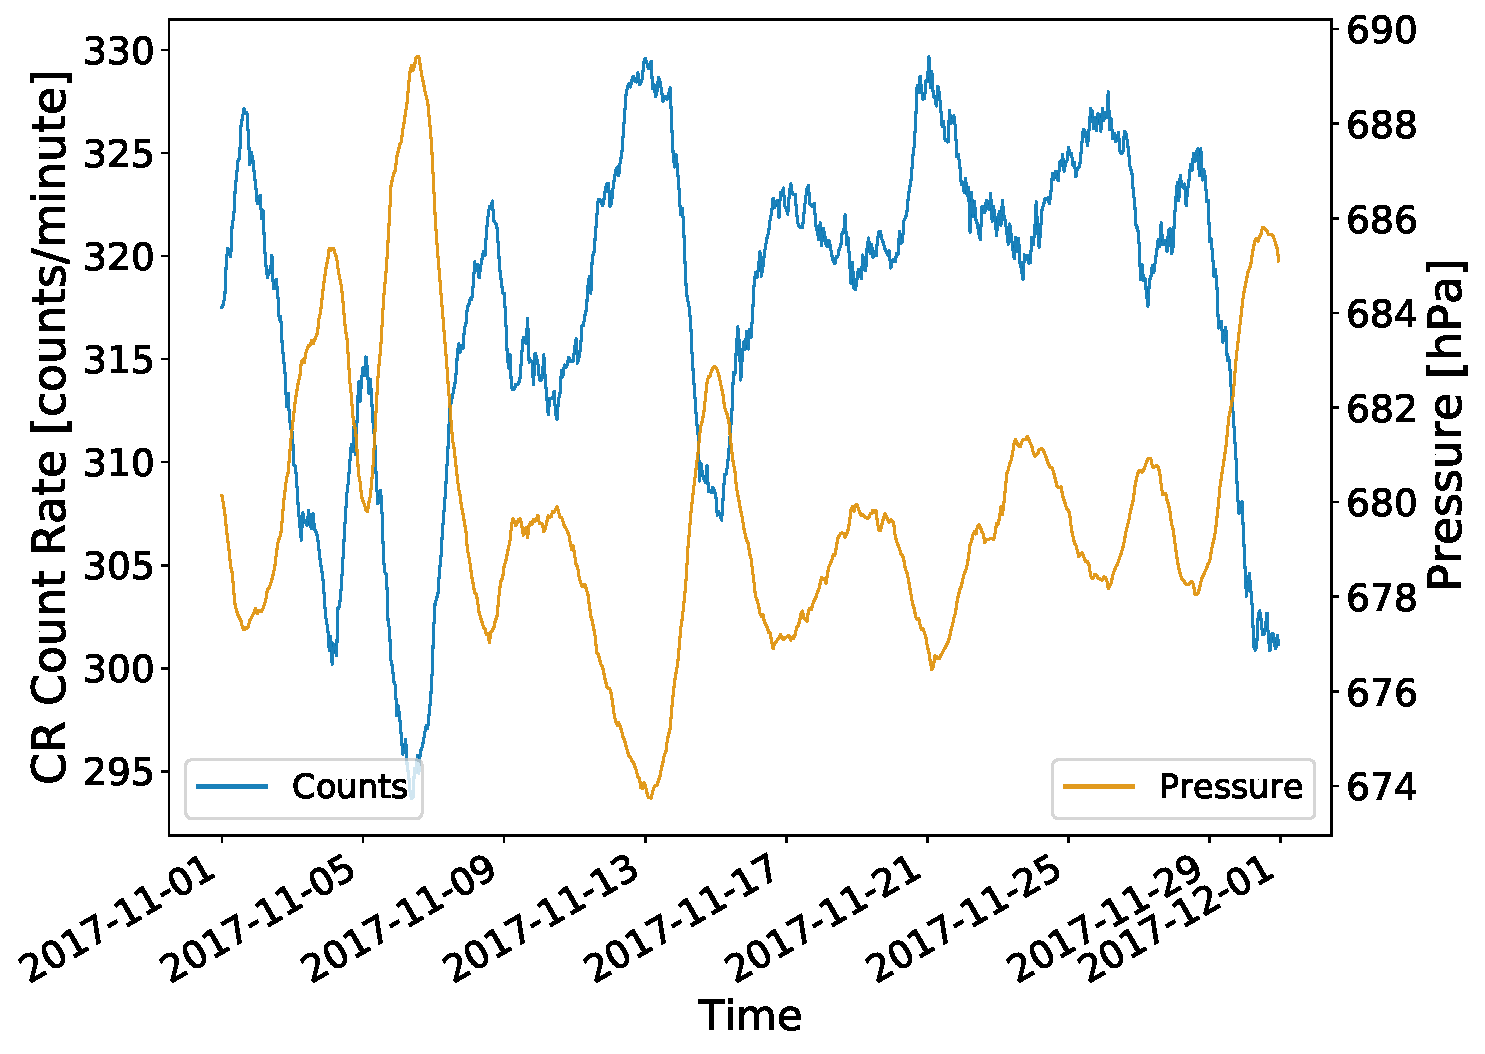
\includegraphics[width=0.48\columnwidth]{SOPO_CRvP.pdf}
		\label{fig:SOPO_CRvP}}
	%\qquad
	\subfloat[HS 501 (Nikhef)]{
		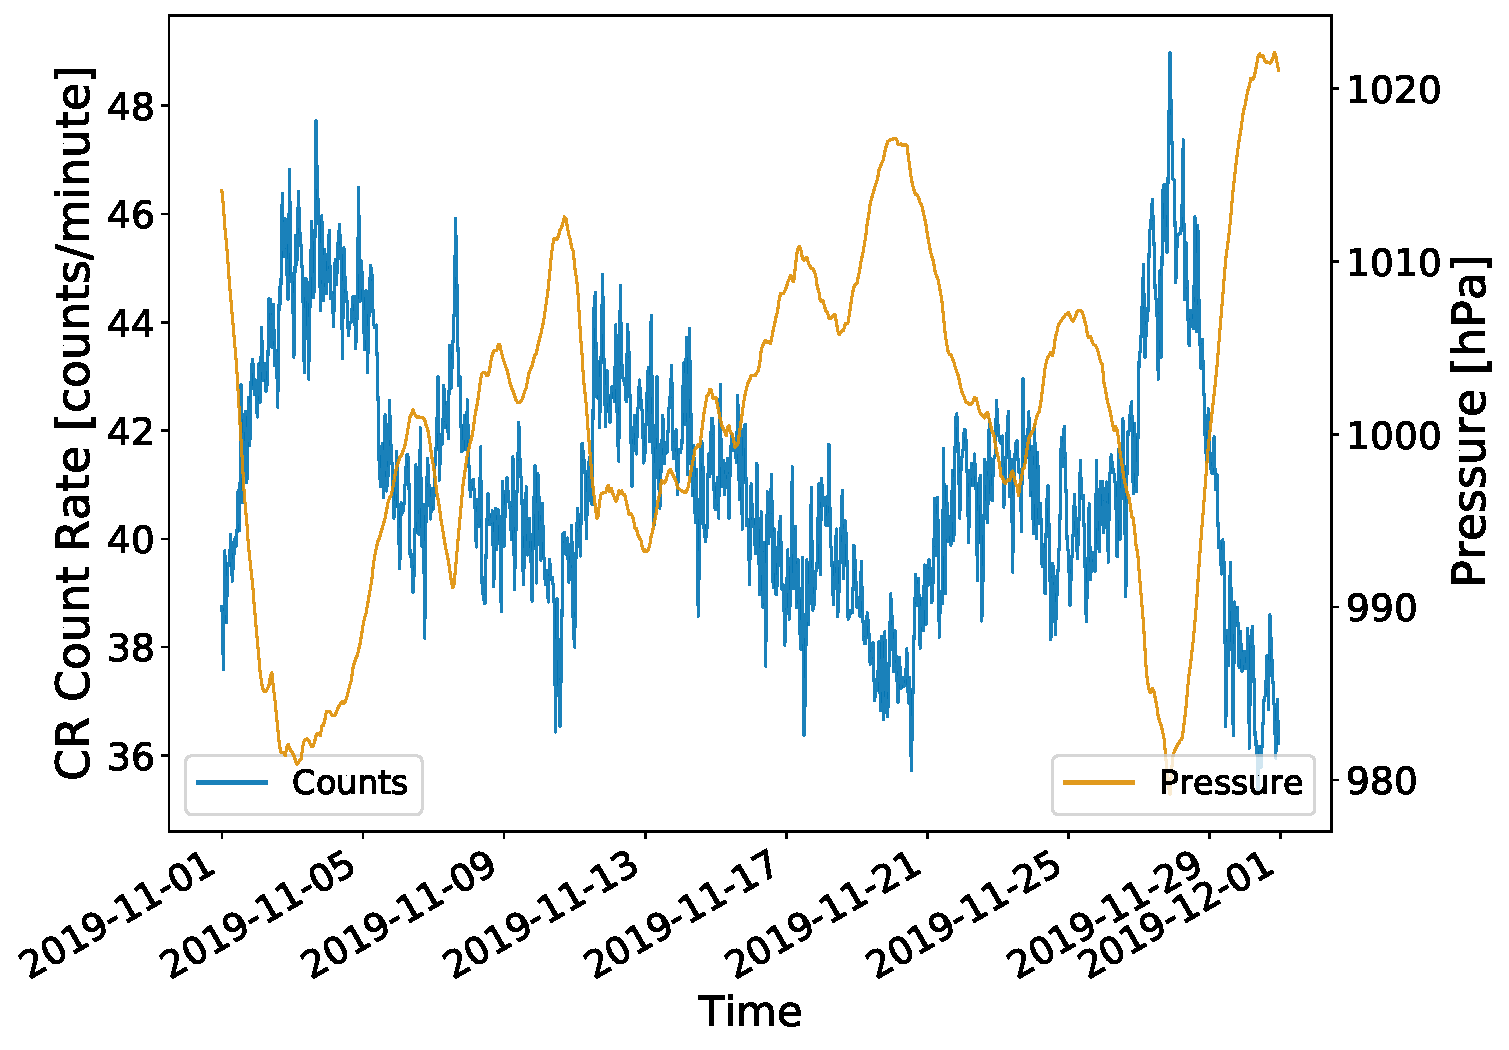
\includegraphics[width=0.48\columnwidth]{501_CRvP.pdf}
		\label{fig:HS_501_CRvP}} \\
	
	\caption{The anti-correlation between CR count rates and the atmospheric pressure. (a) shows the CR and the local atmospheric pressure measured at a NM in the South Pole; (b) shows the CR and pressure measured by HiSPARC station 501. In both plots, the data shown are hourly-averaged, to highlight the effects. The units of time on the x-axis are, YYYY-MM-DD.}
	\label{fig:CR_V_P}
\end{figure}


The method of correcting for the barometric effect is discussed widely in the literature regarding \glspl{nm} and is shown to depend on the barometric coefficient \citep{paschalis_online_2013}. Assuming the cosmic ray flux variation, absent of the atmospheric effects, is reasonably stable, then a simple correction to the counts can be made. The \gls{cr} variations ($N$) that depend on the local atmospheric pressure are described by:

\begin{equation}
\Delta N = - \beta \, N \, \Delta P \, ,
\label{eq:presscorr1}
\end{equation}
%
where $\Delta N$ is the change in count rate, $\beta$ is the barometric coefficient, and $\Delta P = P - P_0$ is the deviation in pressure from the average ($P_0$) in the given time-period \citep{paschalis_online_2013}

Through the integration of equation~(\ref{eq:presscorr1}), the solution shows the dependence of cosmic ray intensity on pressure,

\begin{equation}
N = N_{0} \, e^{-\beta \, \Delta P} \, .
\label{eq:presscorr2}
\end{equation}

Therefore by taking the logarithm of equation~(\ref{eq:presscorr2}), one can obtain the barometric coefficient by fitting the linear model to the observed data, of the form:

\begin{equation}
\mathrm{ln} \left( \frac{N}{N_0} \right) = - \beta \, \Delta P \, ,
\label{eq:presscorr3}
\end{equation}
%
where $N_0$ may be considered as the mean count rate over the given time-period of observations.

A demonstration of this method is shown for both a NM and a \gls{hisparc} station in Figure~\ref{fig:barometric_fit}. In both cases the linear fit does a good job of finding the barometric coefficient and was used to remove the pressure effect from the data.

\begin{figure}[ht!]
	\centering
	\subfloat[SOPO NM Station]{
		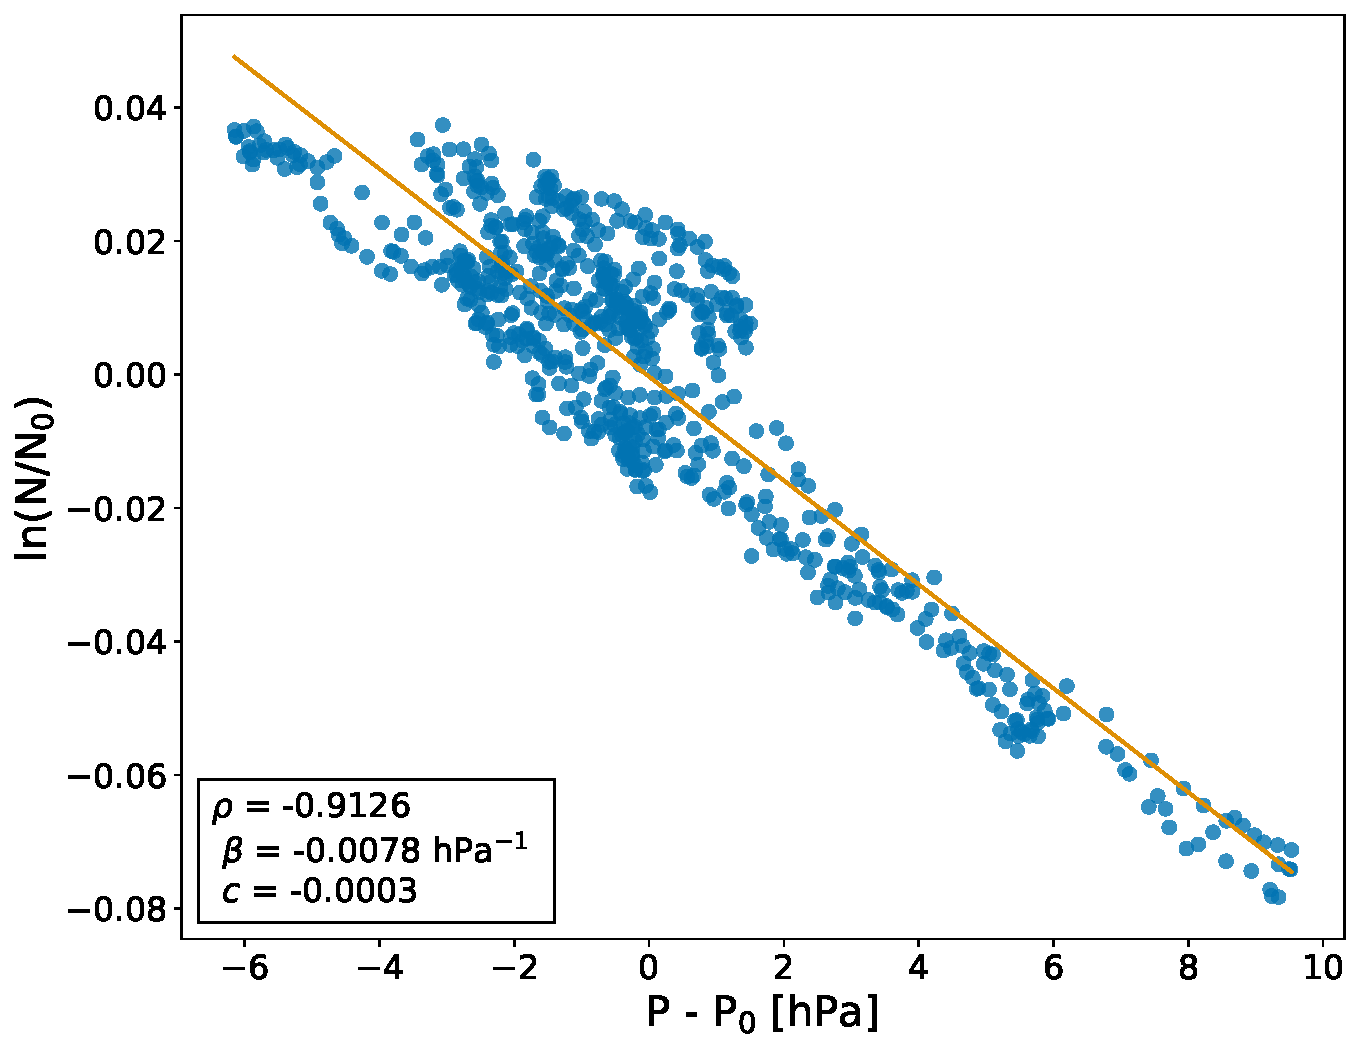
\includegraphics[width=0.48\columnwidth]{SOPO_beta.pdf}
		\label{fig:SOPO_beta}}
	%\qquad
	\subfloat[HS 501 (Nikhef)]{
		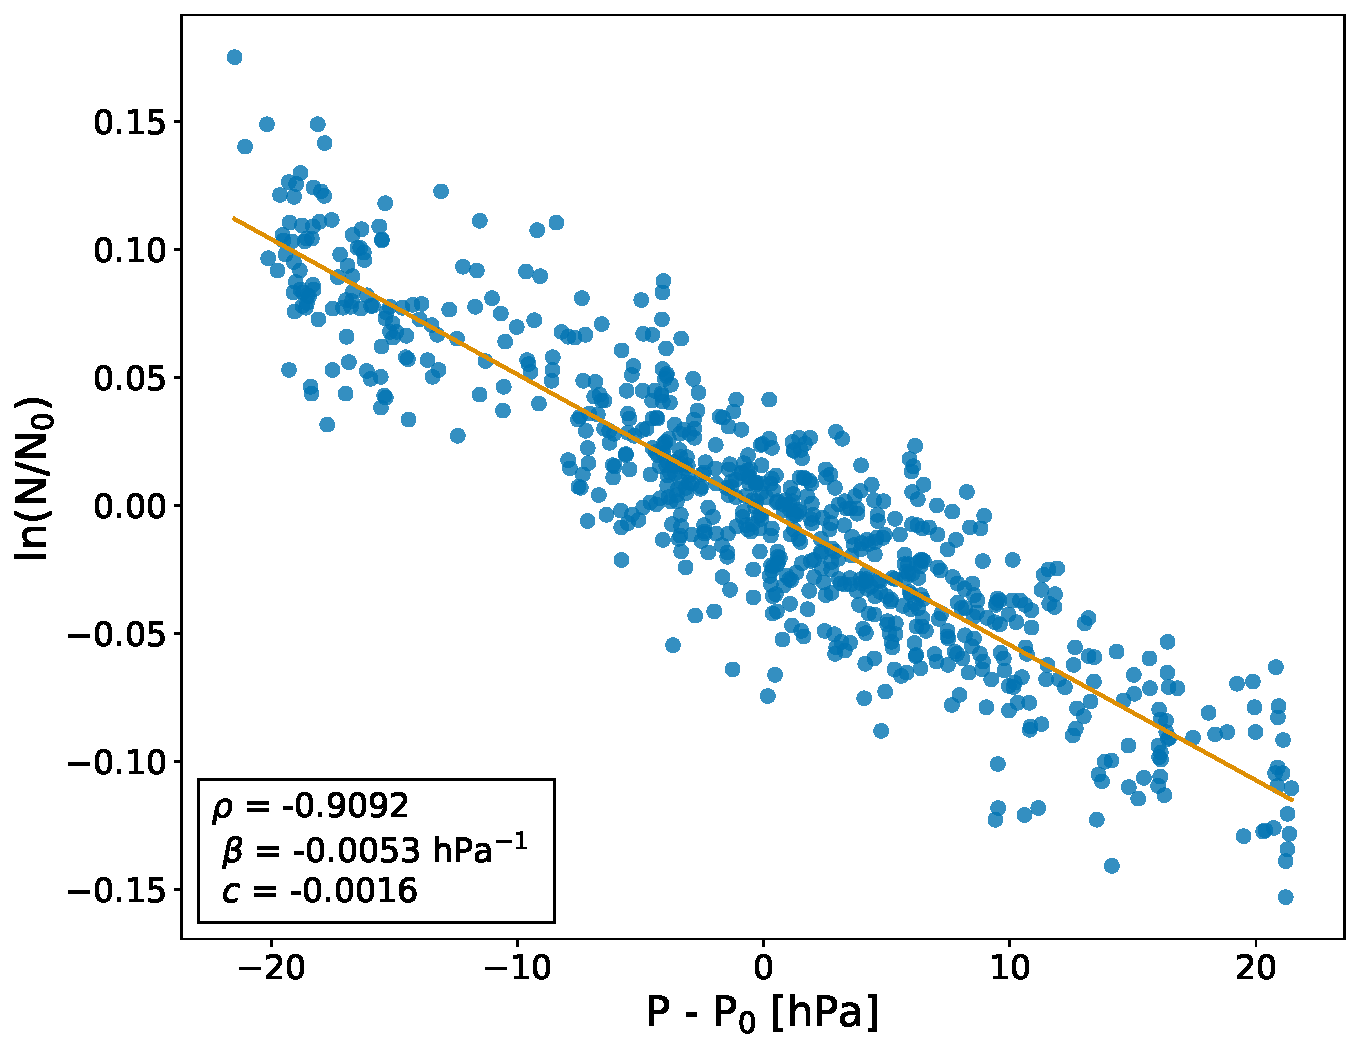
\includegraphics[width=0.48\columnwidth]{501_beta.pdf}
		\label{fig:HS_501_beta}} \\
	
	\caption{The barometric coefficient calculation: (a) during November 2017 for the South Pole (SOPO) NM station, (b) during November 2019 for HiSPARC station 501 at Nikhef.}
	\label{fig:barometric_fit}
\end{figure}

For comparison, and to show the success of this method at removing the pressure variation, the raw and corrected \gls{hisparc} data are shown in Figure~\ref{fig:HS_P_corr}. It is clear from Figure~\ref{fig:HS_P_corr} that the large excursions are adequately removed from the data after the correction.

\begin{figure}[ht!]
	\centering
	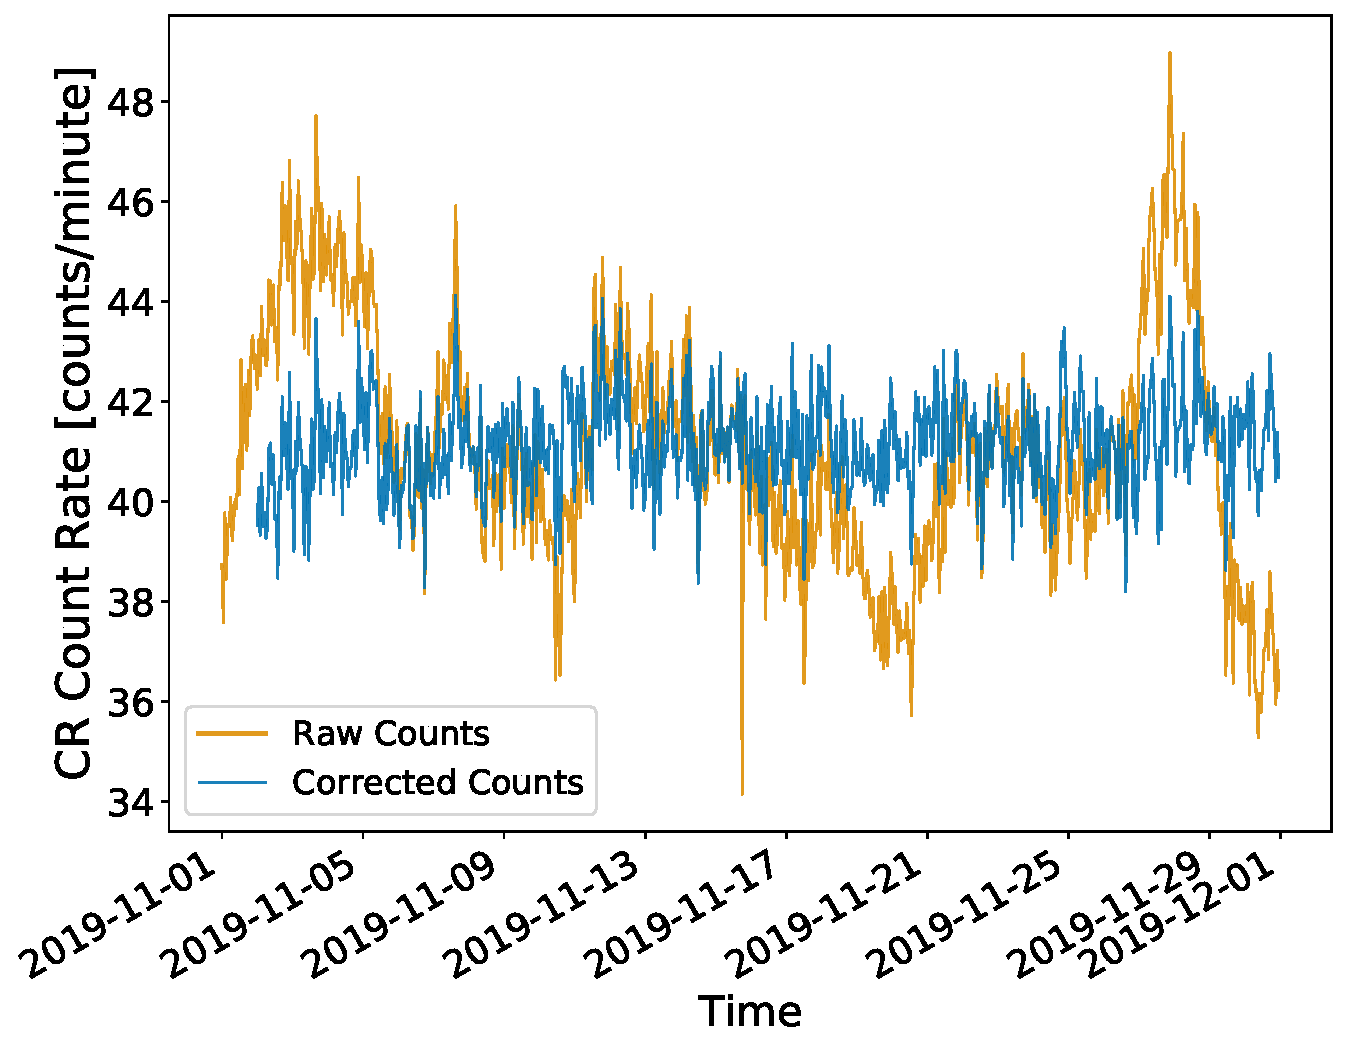
\includegraphics[width=0.65\columnwidth]{501_raw_vs_corrected.pdf}
	\caption{A comparison between the hourly-averaged HiSPARC count rate before (orange line) and after the pressure correction (blue line). The units of time on the x-axis are, YYYY-MM-DD.}
	\label{fig:HS_P_corr}
\end{figure}


Using the online barometric coefficient tool \citep{paschalis_online_2013}, it was possible to also provide a comparison between the method used in this work and the correction of the \gls{nmdb} stations, as a further validation. This is shown in Figure~\ref{fig:NM_beta_variation} for monthly corrections throughout 2017 for the \gls{nm} station at the South Pole (SOPO).

\begin{figure}[ht!]
	\centering
	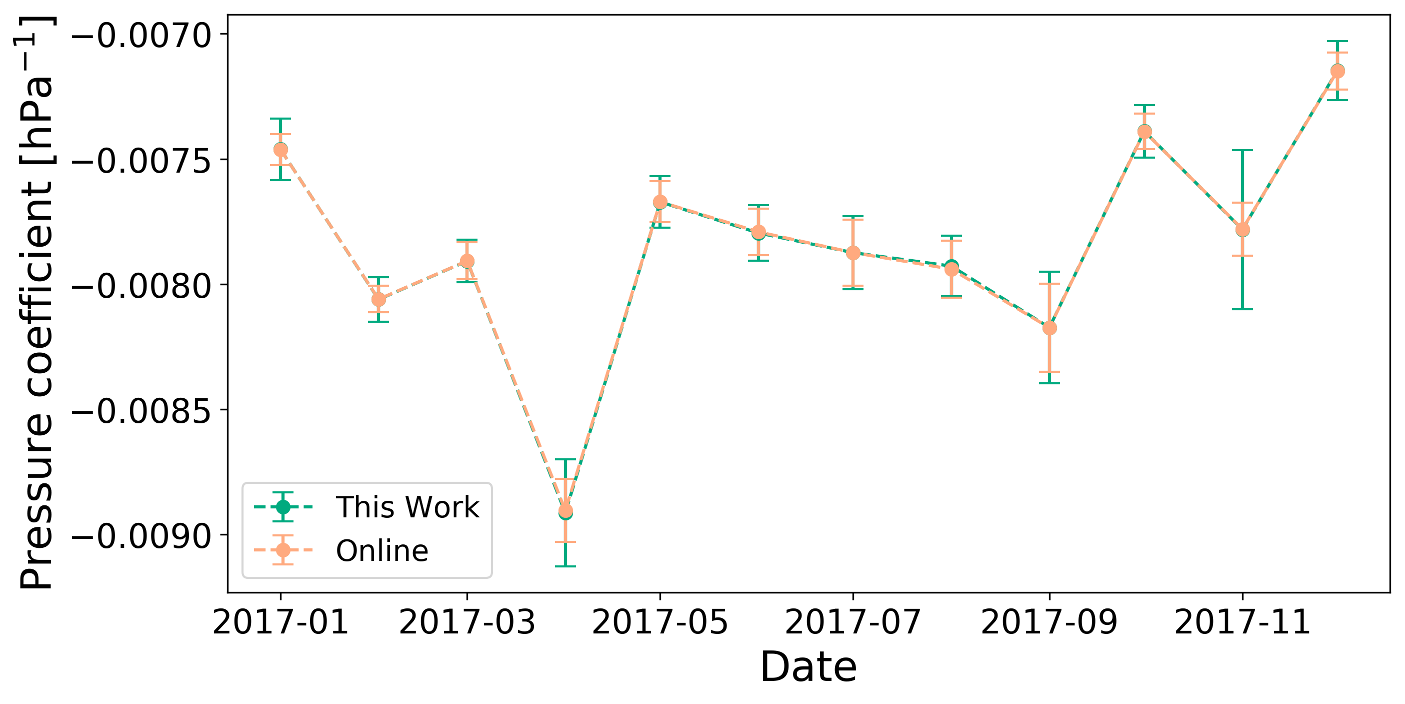
\includegraphics[width=0.75\columnwidth]{SOPO_beta_2017_rescale.png}
	\caption{A comparison between the monthly barometric coefficient computed in this work and using the online barometric coefficient tool throughout the year 2017 for the SOPO NM station. The units of time on the x-axis are, YYYY-MM.}
	\label{fig:NM_beta_variation}
\end{figure}


Figure~\ref{fig:NM_beta_variation} shows a close agreement between the barometric coefficient calculated in this work and those acquired from the online tool for the SOPO \gls{nm}. This was also true for other stations tested (Apatity and Rome), thus validating that the method used in this work was suitable for application on the \gls{hisparc} data. The barometric correction was performed on the \gls{hisparc} data for stations where sufficient pressure data and count rates existed.
%As this method has been shown to reproduce the results of the \gls{nmdb} corrections the barometric correction and adequately remove the correlated excursions due to pressure, it was performed on the stations where sufficient pressure data and count rates exist. % were re-investigated to determine whether the space weather events were observed in the \gls{hisparc} data. These results are provided in Section \ref{sec:HS_obs_Pcorr}.





%%%%%%%%%%%%%%%%%%%%%%%%%%%%%%%%%%%%%%%%%%%%%%%%%%%%%%%%%%%%%%%%%%%%%
\subsection{Temperature Correction}\label{sec:HS_T_corr}

The effects of atmospheric temperature have been shown to influence both the creation and disintegration processes for muons in the atmosphere \citep{berkova_temperature_2011}. There is hence a positive effect and a negative effect on muon intensity as a consequence of temperature variations \citep{mendoncca_temperature_2016}. 

The positive effect is related to pion decay and its dependence on temperature variation. The higher the temperature, the lower the atmospheric pion absorption, which implies a higher generation rate of muons \citep{mendoncca_temperature_2016}.

The negative effect corresponds to the decrease of muon intensity at ground level as the muon average path length varies with temperature. Due to the heating and expansion of the atmosphere during summer periods muons are produced higher in the atmosphere; hence the muon propagation path length increases meaning there is more atmosphere for muons to traverse before reaching the ground, and an increased decay probability and ionisation losses \citep{savic_pressure_2015, mendoncca_temperature_2016}.

Due to the difference in decay probability, the negative effect dominates for low energy muons and the positive effect dominates for high energy muons \citep{berkova_temperature_2011}. It is therefore expected that the negative effect should dominate for the \gls{hisparc} network. This is in contradiction with the observations of diurnal variation with the \gls{hisparc} detectors, as one can quite clearly see that the \gls{hisparc} stations register higher count rates during local noon (see Fig.~\ref{fig:GLE72_8001}). However, when observing the singles rates, we do see some detectors displaying a positive effect and some displaying a negative effect (see Fig.~\ref{fig:GLE_72}). This is not consistent between stations, and provides more evidence to suggest this is an effect of thermally induced noise in the \glspl{pmt}. %Temperature effects are also observed by NMs; however, the effect is less significant than for MDs hence temperature corrections are not widely applied for NMs \citep{mendoncca_temperature_2016}.


Several methods of correcting for the temperature effect are discussed in the literature, e.g. see \citet{berkova_temperature_2011} and \citet{mendoncca_temperature_2016} for a summary. However, the methods discussed are typically applied over long timescales of years, to account for seasonal variations with low temporal resolution, rather than to account for short timescale variations with periods of less than a day; hence these methods are not necessarily suitable for this work on ephemeral space weather events.

%Several methods of correcting for the negative temperature effect are summarised by \cite{berkova_temperature_2011} which utilise different measures of atmospheric temperature when performing the temperature correction. \cite{mendoncca_temperature_2016} provides a comparative summary of these methods applied to correct for atmospheric temperature variations observed by GMDN detectors. The methods discussed here however are typically applied over long timescales of years with low temporal resolution rather than to account for short timescale variations with periods of less than a day; hence these methods aren't necessarily suitable for this work on ephemeral space weather events.

%\cite{mendoncca_temperature_2016} concludes that correcting for temperature using the atmospheric mass weighted temperature is one of the most suitable methods for the GMDN as it allows for the highest correlation between long-term \gls{cr} variations and temperature. The mass weighted method is an approximation for integrating over the vertical atmospheric temperature as is given in Eq. (\ref{eq:tempcorr}):
%
%\begin{equation}
%\left( \frac{\Delta N}{N} \right)_T = \, \bar{\alpha}  \int^{h_0}_{0}  \, \delta \, T(h) \, dh = \sum_{i=0}^{n} \frac{x(h_i) - x(h_{i+1})}{x(h_0)} T(h_i)  = \alpha_{\mathrm{MSS}} \delta T_{\mathrm{MSS}}
%\label{eq:tempcorr}
%\end{equation}
%
%where $h_0$ is the closest to ground altitude; $\delta T_{\mathrm{MSS}}$ is the deviation of the mass weighted atmospheric temperature; $T(h_i)$ is the temperature in degrees kelvin observed at the altitude $h_i$; $x(h_ i)$ is the atmospheric depth at the altitude $h_i$ which is given by Eq. \ref{eq:atmos_depth}:
%
%\begin{equation}
%x(h) = \int^{\infty}_{h}  \, \rho (h) \, dh  \, \rho (h) = \frac{P(h)}{T(h)} \frac{M_{mol}}{R} 
%\label{eq:atmos_depth}
%\end{equation}
%
%where $P(h)$ is the atmospheric pressure profile as a function of depth; $T(h)$ is the atmospheric temperature; $\rho(h)$ is the air density at a given altitude $h$; $M_{mol}$ is the molar mass of air; $R$ is the universal gas constant.
%
%The temperature correction is therefore used in a formalism the same as Eq. (\ref{eq:presscorr3}), replacing replacing $\beta$ for $\alpha$ and $\Delta P$ for $\Delta T$.
%
%In addition it is discussed by \cite{berkova_temperature_2011} and \cite{mendoncca_temperature_2016} that the effective generation level temperature is a suitable assumption for this purpose. This method is based on the assumption that muons are mostly generated at a certain isobaric level, taken as 100 mbar, and therefore the temperature at 100 mbar in the atmospheric pressure profile is used, $T_{\mathrm{100 \, mbar}}$.
%
%As discussed above, \cite{mendoncca_temperature_2016} provide this as a method for correcting for the long-term variation in atmospheric temperature which varies seasonally rather than to correct for diurnal variations; therefore it is unsure how relevant this method of atmospheric temperature correction will be to the diurnal variations observed in the HiSPARC data.

The \gls{hisparc} stations provide the local outdoor temperature which is measured nearby the detectors and also the temperature in the room where the electronics are located. The latter is not of use, but the former can be used for temperature corrections. Figure~\ref{fig:HS_8001_CRvT} shows the pressure corrected events data and the temperature data for station 8001 in July 2012. There is a strong correlation between the events and the temperature, which is demonstrated in Figure~\ref{fig:HS_8001_alpha}, yet weaker than with pressure.

\begin{figure}[ht!]
	\centering
	\subfloat[Pressure corrected CR counts and temperature data comparison]{
		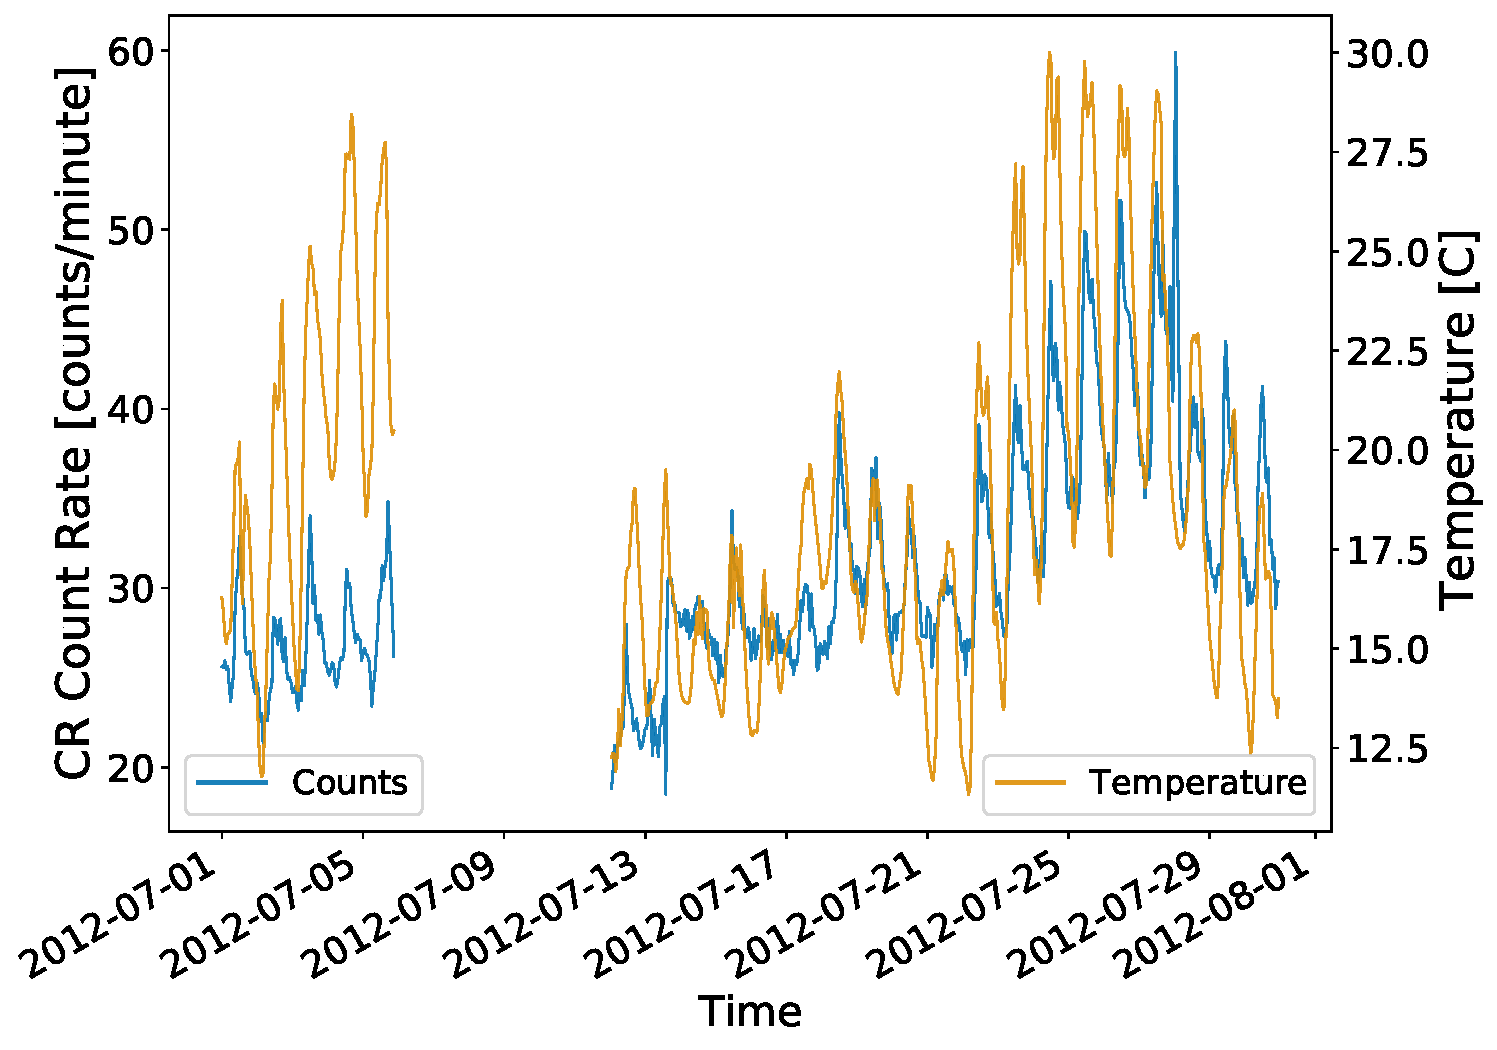
\includegraphics[width=0.48\columnwidth]{8001_CRvT.pdf}
		\label{fig:HS_8001_CRvT}}
	%\qquad
	\subfloat[Corrlation between CR counts and temperature]{
		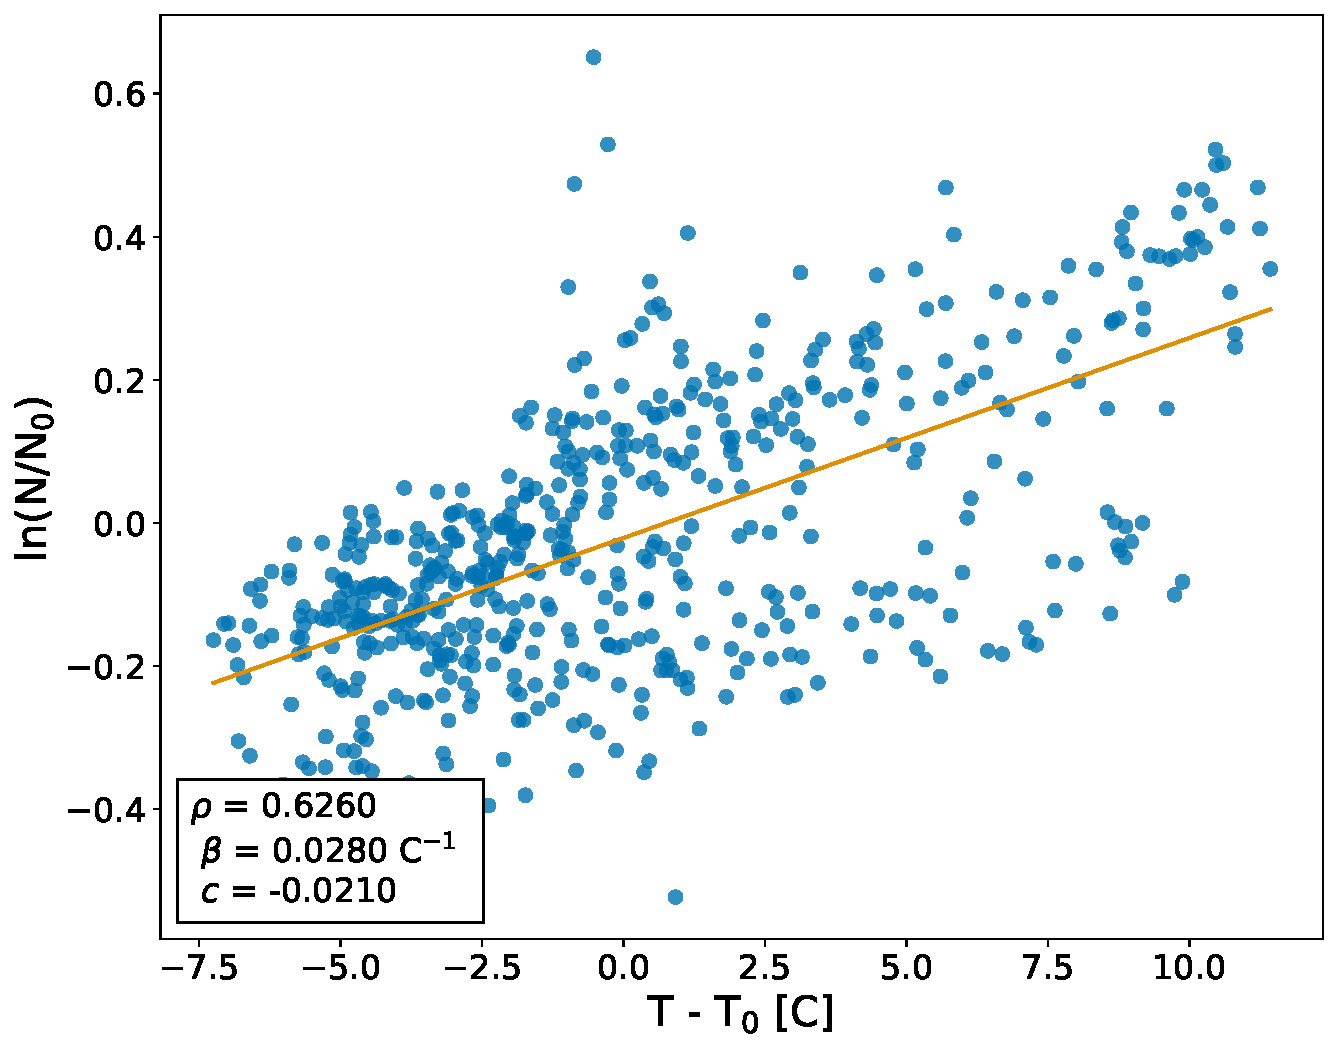
\includegraphics[width=0.48\columnwidth]{8001_alpha.pdf}
		\label{fig:HS_8001_alpha}} \\
	
	\caption{The relationship between the pressure corrected events data and the outdoor temperature as measured at HiSPARC station 8001 (Eindhoven). (a) shows the time-series of hourly-averaged pressure corrected events and temperature data; (b) shows the correlation between the counts and temperature, and the fitted line to calculate the correction coefficient.}
	\label{fig:CR_V_T}
\end{figure}

We simplified the correction method and used a linear fitting technique (i.e. the same as the barometric correction in Section~\ref{sec:HS_P_corr}; however, replacing the pressure for locally measured outdoor temperature). We can see from Figure~\ref{fig:HS_T_corr} that this correction method does remove a significant amount of the variation correlated with the outdoor variation, including dampening the strong diurnal variation. There still persists some strong variation in the count rate however, which shows that this method is not as effective as the pressure correction. Nevertheless, we continue with this temperature correction as it is sufficient at reducing the diurnal variation in the data around the events considered.
%Despite the literature, we used the same linear fitting technique described for the pressure correction in Section~\ref{sec:HS_P_corr}; however, replacing the pressure for locally measured outdoor temperature. We can see from Figure~\ref{fig:HS_T_corr} that this correction method does remove a significant amount of the variation correlated with the outdoor variation, including dampening the strong diurnal variation. There still persists some strong variation in the count rate however, which shows that this method is not as effective as the pressure correction. Nevertheless, we continue with this temperature correction as it is sufficient at reducing the diurnal variation in the data around the events considered.
 
\begin{figure}[ht!]
	\centering
	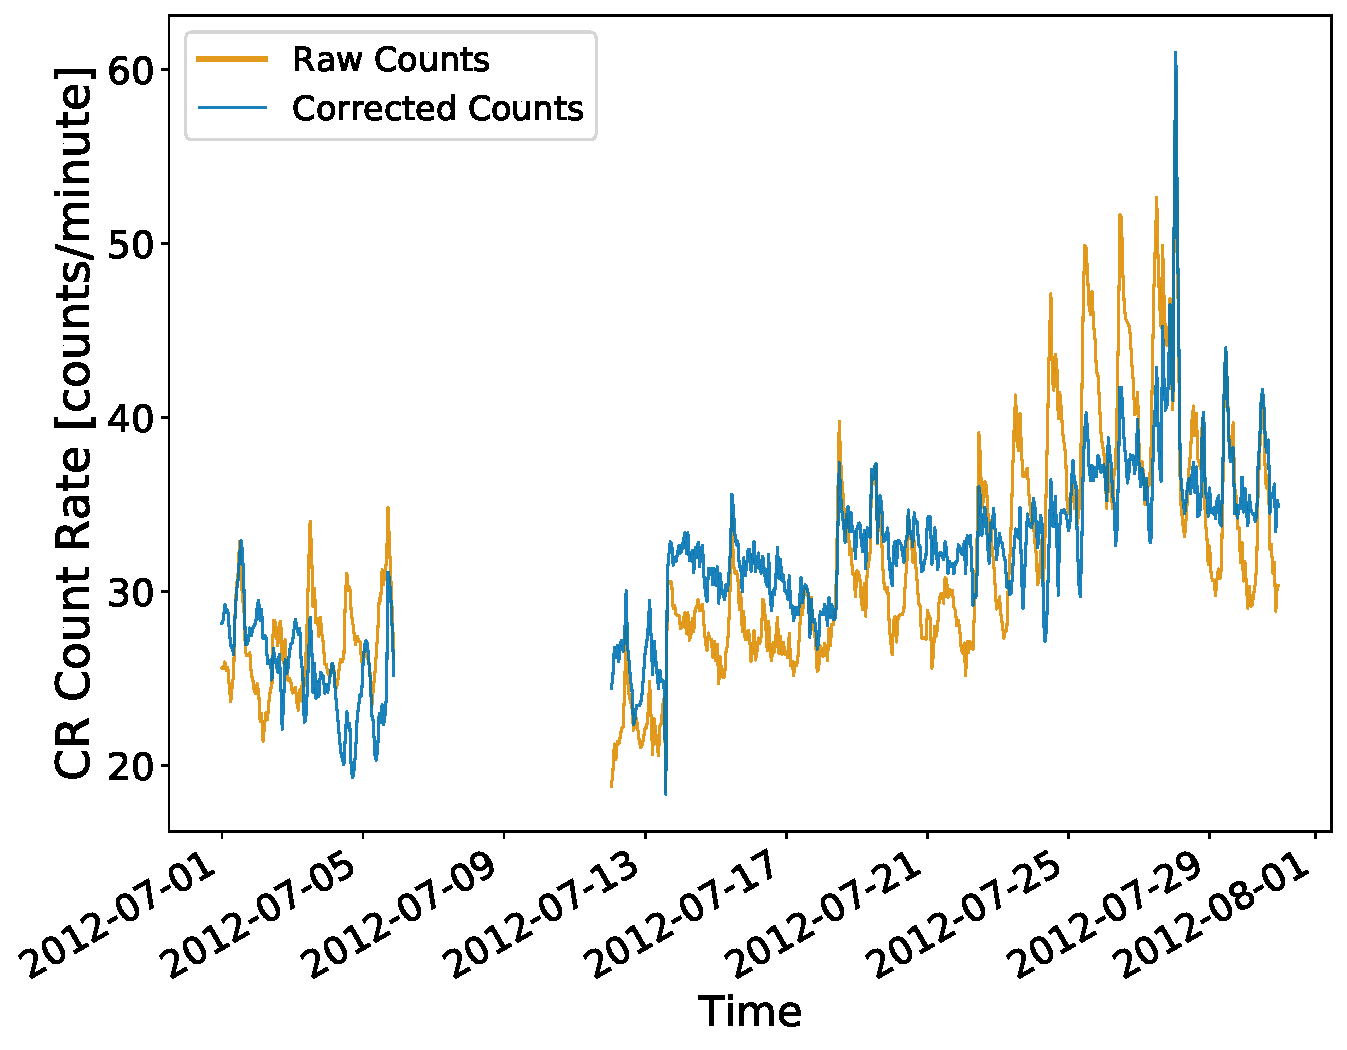
\includegraphics[width=0.65\columnwidth]{8001_raw_vs_corrected.pdf}
	\caption{A comparison between the hourly-averaged HiSPARC count rate before (orange line) and after the temperature correction (blue line). After the correction, the diurnal variation from the temperature effect has been reduced.}
 	\label{fig:HS_T_corr}
\end{figure}
 

 

%%%%%%%%%%%%%%%%%%%%%%%%%%%%%%%%%%%%%%%%%%%%%%%%%%%%%%%%%%%%%%%%%%%%%
%%%%%%%%%%%%%%%%%%%%%%%%%%%%%%%%%%%%%%%%%%%%%%%%%%%%%%%%%%%%%%%%%%%%%
\section{HiSPARC Observations After Atmospheric Corrections}\label{sec:HS_obs_Pcorr}


%%%%%%%%%%%%%%%%%%%%%%%%%%%%%%%%%%%%%%%%%%%%%%%%%%%%%%%%%%%%%%%%%%%%%
\subsection{Observations of Ground Level Enhancements}

Following the atmospheric correction, the search for evidence of \glspl{gle} was repeated, this time within the corrected \gls{hisparc} data. This could only be done for \gls{gle} 71 and 72, as the \gls{hisparc} network was not collecting meteorological data during the epoch of \gls{gle} 70. Figure~\ref{fig:GLE_71_Pcorr} and Figure~\ref{fig:GLE_72_Pcorr} show the atmospheric-effect corrected \gls{hisparc} observations around the epochs of \gls{gle} 71 and 72, respectively. The observations of \gls{gle} 71 show only the \gls{hisparc} events data; however, we also show the singles rates from each of the individual detectors in a station for \gls{gle} 72.

\begin{figure}[ht!]
	\centering
	\subfloat[HS 3001 (Leiden)]{
		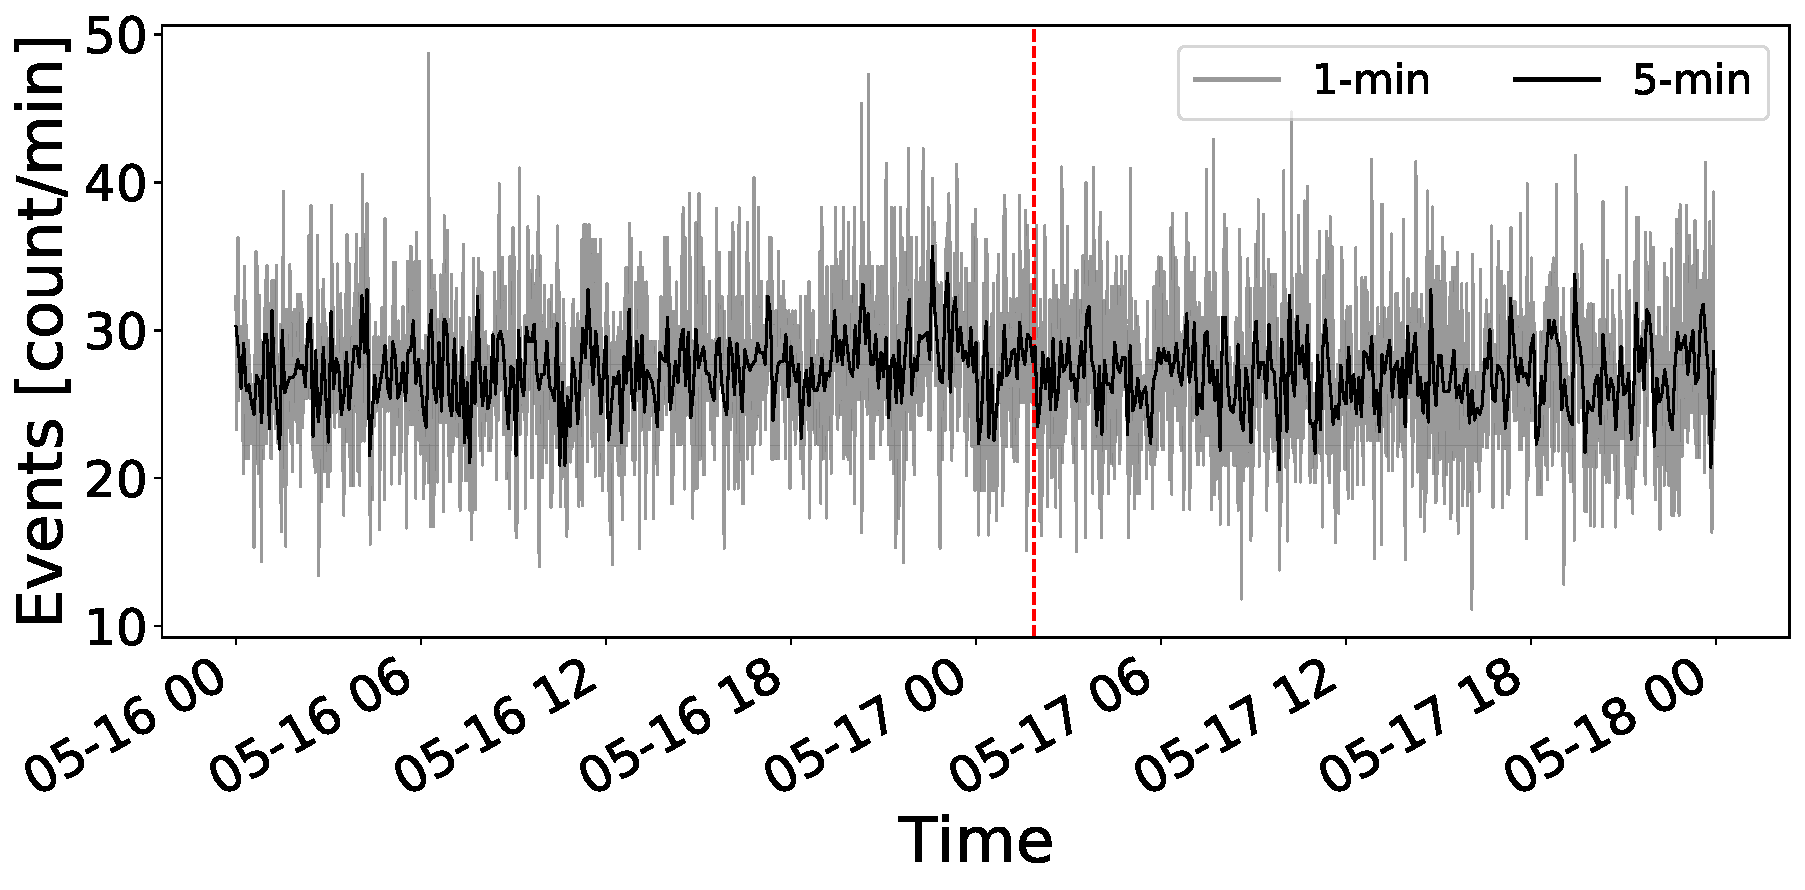
\includegraphics[width=0.48\columnwidth]{GLE71_3001_CORR.pdf}
		\label{fig:GLE71_3001_Pcorr}}
	%\qquad
	\subfloat[HS 8001 (Eindhoven)]{
		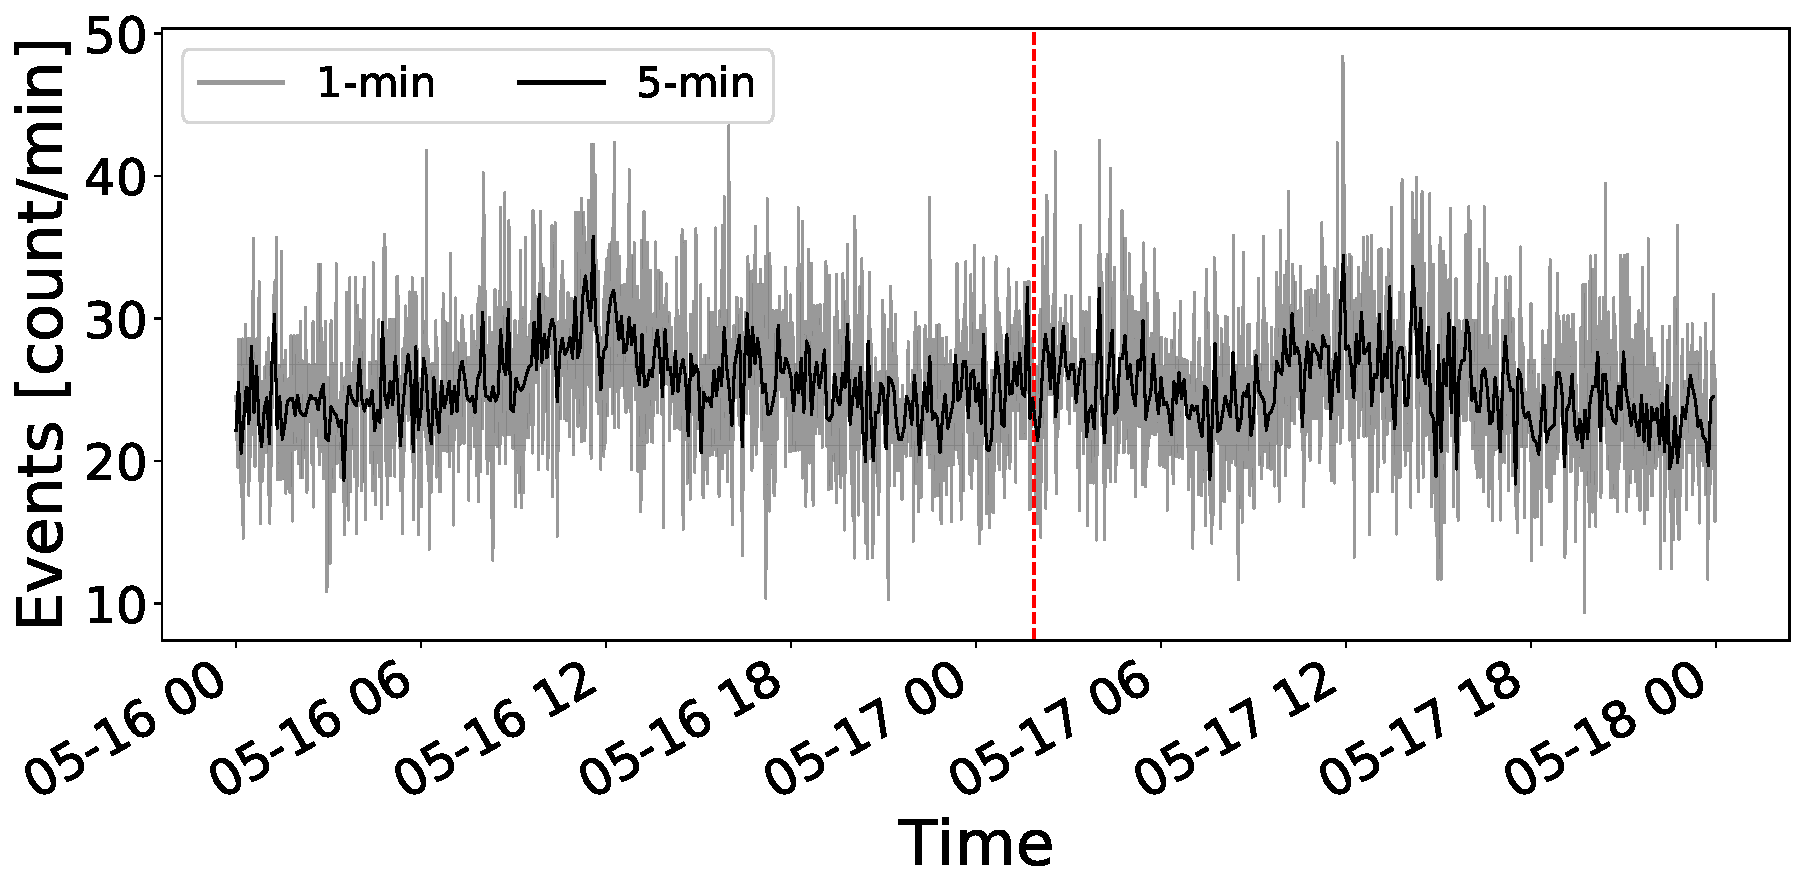
\includegraphics[width=0.48\columnwidth]{GLE71_8001_CORR.pdf}
		\label{fig:GLE71_8001_Pcorr}} \\
	
	
	\caption{Atmospheric-corrected HiSPARC data for stations 8001 and 3001 around the epoch of GLE 71 on 17/05/2012. The plot shows the minute-averaged (grey) and 5-minute-averaged (black) trigger events between detectors within the station. The vertical red, dashed line depicts the approximate onset time of the GLE. The units of time on the x-axis are, MM-DD HH.}
	\label{fig:GLE_71_Pcorr}
\end{figure}
%
%
%
\begin{figure}[ht!]
	\centering
	\subfloat[HS 501 (Nikhef)]{
		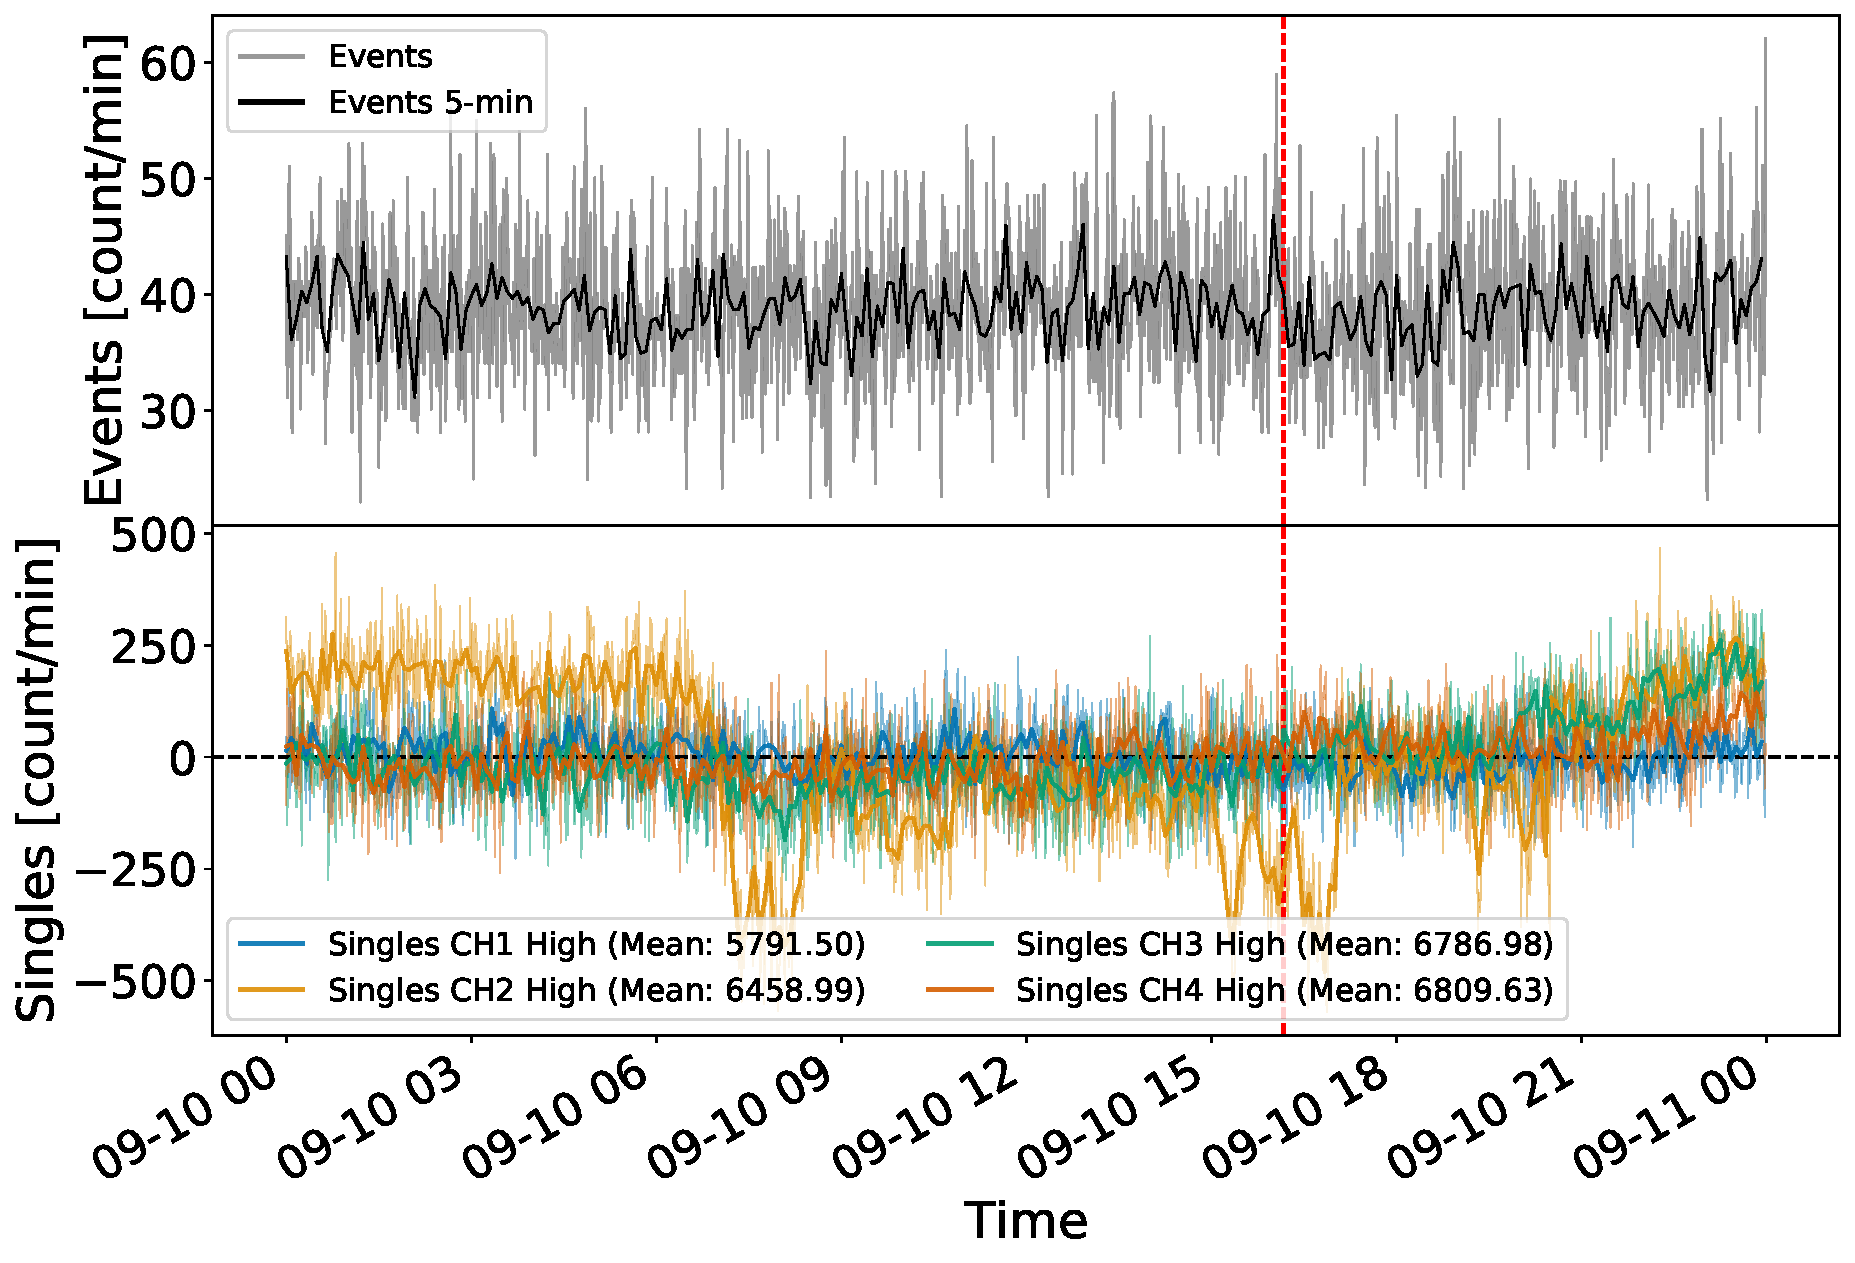
\includegraphics[width=0.48\columnwidth]{GLE72_501_CORR.pdf}
		\label{fig:GLE72_501_Pcorr}}
	%\qquad
	\subfloat[HS 203 (College Hageveld)]{
		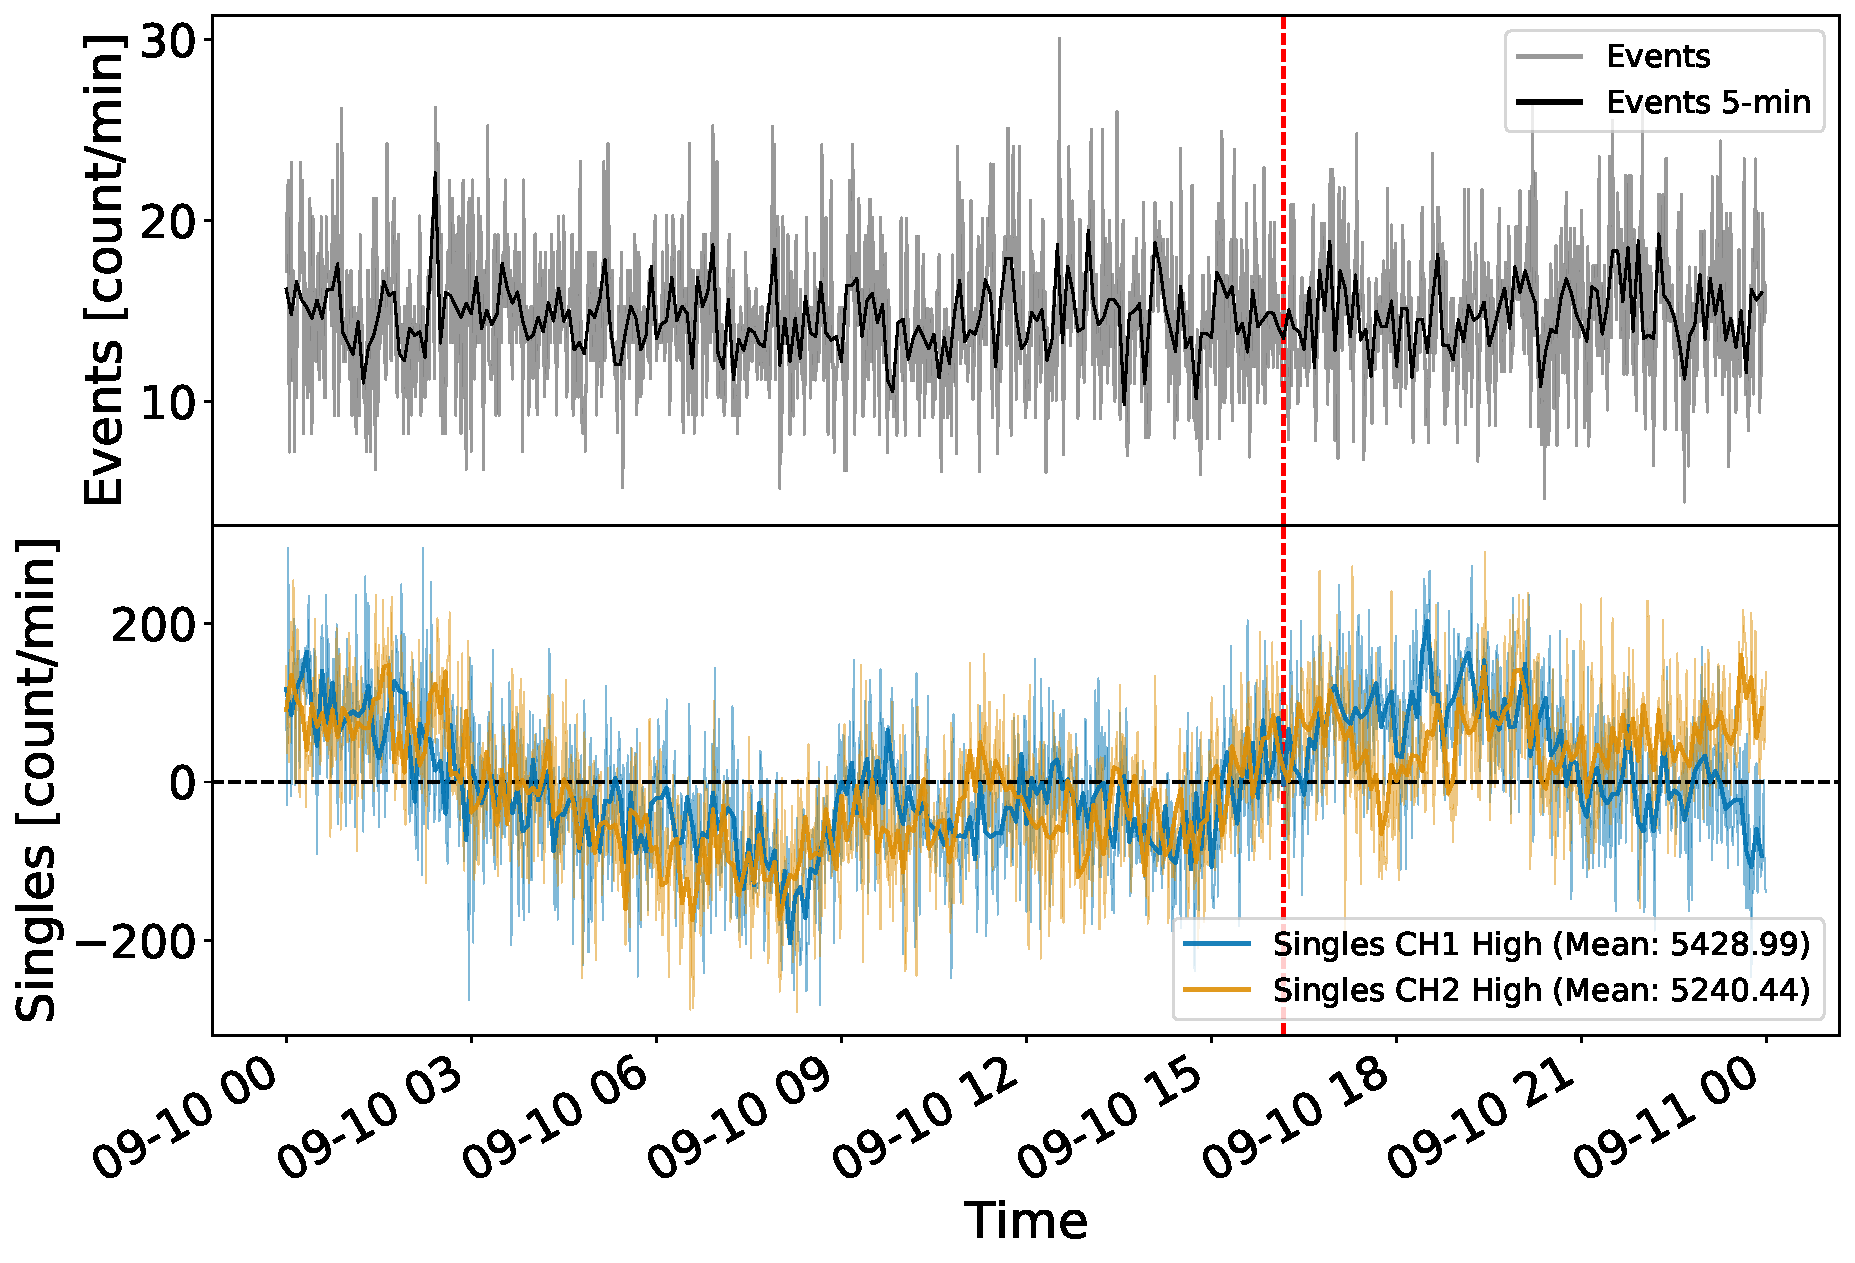
\includegraphics[width=0.48\columnwidth]{GLE72_203_CORR.pdf}
		\label{fig:GLE72_203_Pcorr}} \\
	
	
	\caption{Atmospheric-corrected HiSPARC data for 2 stations around the epoch of GLE 72 on 10/09/2017. The top panel of each subplot shows the minute-averaged (grey) and 5-minute-averaged (black) trigger events between detectors within the station, while the bottom panel shows the 1- and 5-minute averaged singles counts, mean-subtracted, for each individual detector (or signal channel, CH$n$) in the station. The vertical red, dashed line depicts the approximate onset time of the GLE. The units of time on the x-axis are, MM-DD HH.}
	\label{fig:GLE_72_Pcorr}
\end{figure}

Despite the atmospheric correction, in general, doing a good job at removing atmospheric variations in the \gls{cr} counts, there still remained no clear \glspl{gle} observations in the pressure corrected \gls{hisparc} data. We believe this is due to a mixture of the reasons discussed above. A high rigidity cut-off of the \gls{hisparc} stations leads to a low increase in the \gls{cr} count, as \glspl{gle} are typically caused by \glspl{sep} with a lower energy; hence too few additional muons were produced during the \glspl{gle}. Again we should however note that \citet{humble_j._e._detection_2012} stated that \gls{nm} stations with cut-off rigidities up to $\sim 15$~GV observed the \gls{gle} in September 1989, indicating that high-energy \glspl{sep} may be present and also cause \glspl{gle}, suggesting the rigidity cut-off may not be the limiting factor. In addition, as discussed above, the events data require a trigger between 2 detectors that are separated by up to 10~m, therefore this further biases the stations to be sensitive to more energetic \glspl{pcr}. Furthermore, the issue could be due to the particle species, re-emphasising the wide use of \glspl{nm} rather than \glspl{md}.

This provides motivation to investigate the flux of muons at ground level during quiet periods, i.e. from \glspl{gcr}, compared to the flux of muons at ground level during energetic solar events such as \glspl{gle}. This work was performed and is discussed in Section~\ref{sec:CORSIKA}.


%%%%%%%%%%%%%%%%%%%%%%%%%%%%%%%%%%%%%%%%%%%%%%%%%%%%%%%%%%%%%%%%%%%%%
\subsection{Observations of Forbush Decreases}

The search for evidence of \glspl{fd} was also re-conducted using the atmospheric-effect corrected \gls{hisparc} data. Figure~\ref{fig:FD_201207_8001_Pcorr} and Figure~\ref{fig:FD_201412_501_Pcorr} shows the corrected \gls{hisparc} observations around the epochs of a \gls{fd} in July 2012 and December 2014, respectively.

\begin{figure}[ht!]
	\centering
	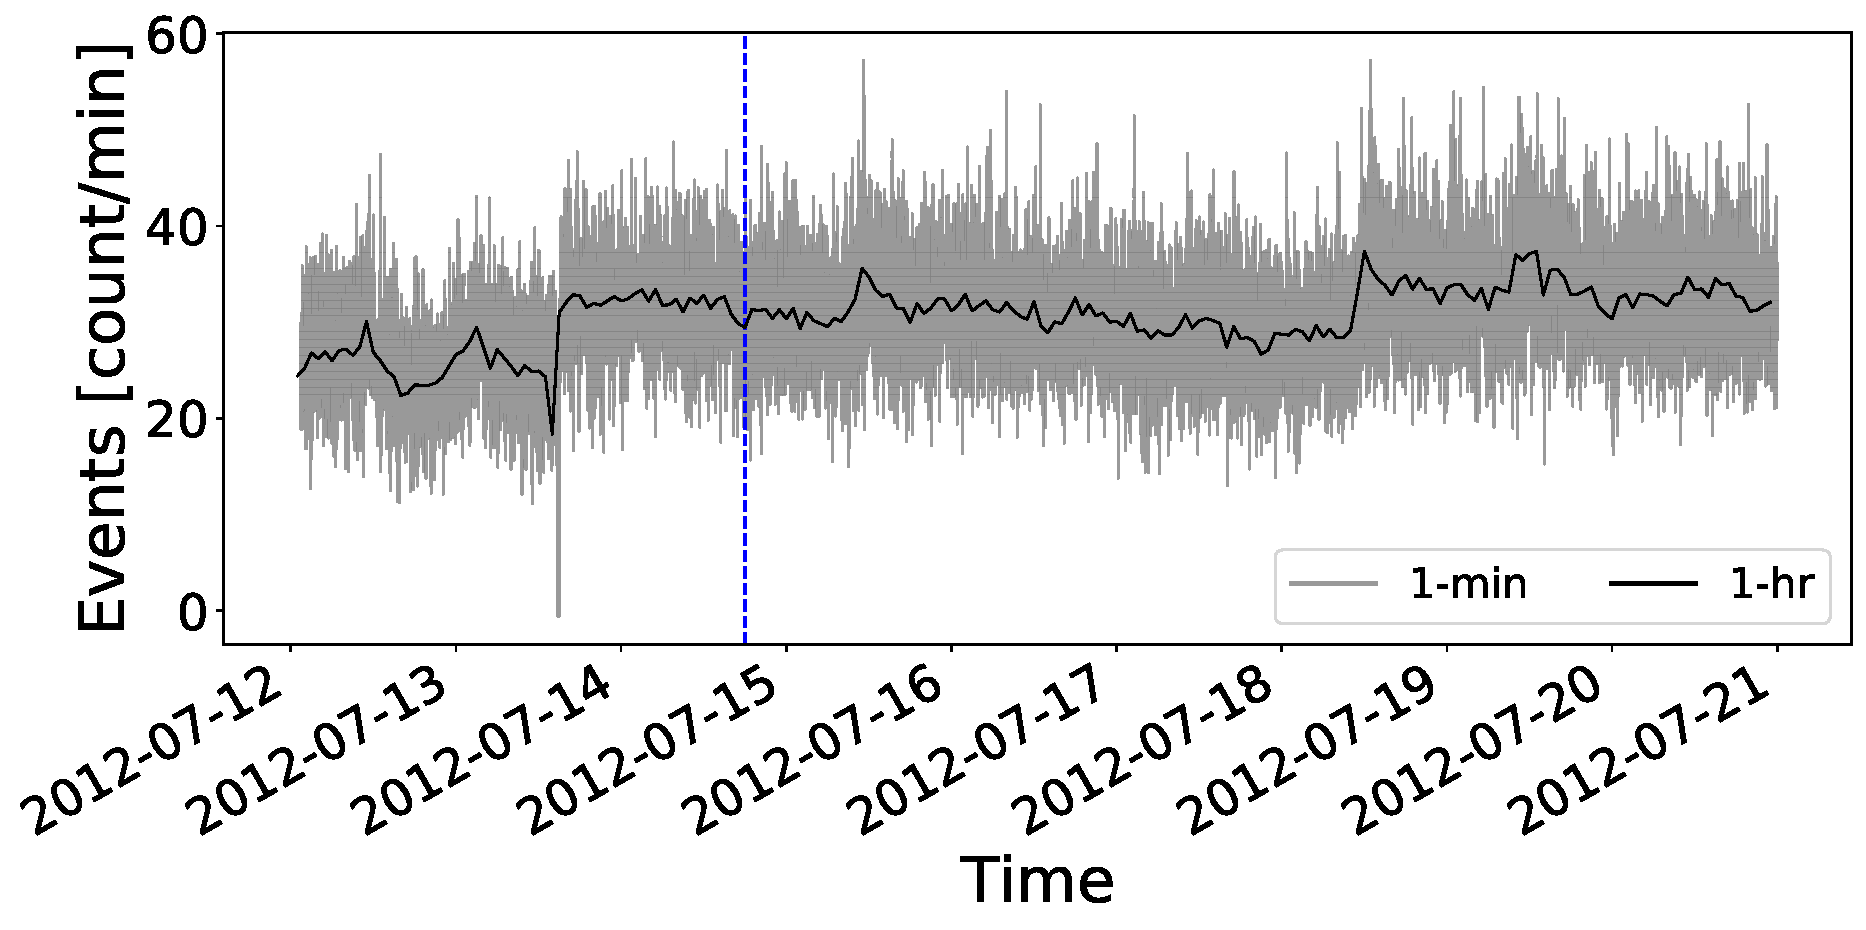
\includegraphics[width=0.65\columnwidth]{FD_201207_8001_CORR.pdf}
	\caption{Atmospheric-corrected HiSPARC data for station 8001 (Eindhoven) around the epoch of the FD in July 2012. The plot shows the minute-averaged (grey) and hourly-averaged (black) trigger events between detectors within the station. The vertical blue, dashed line depicts the approximate onset time of the FD. The units of time on the x-axis are, YYYY-MM-DD.}
	\label{fig:FD_201207_8001_Pcorr}
\end{figure}
%
\begin{figure}[ht!]
	\centering
	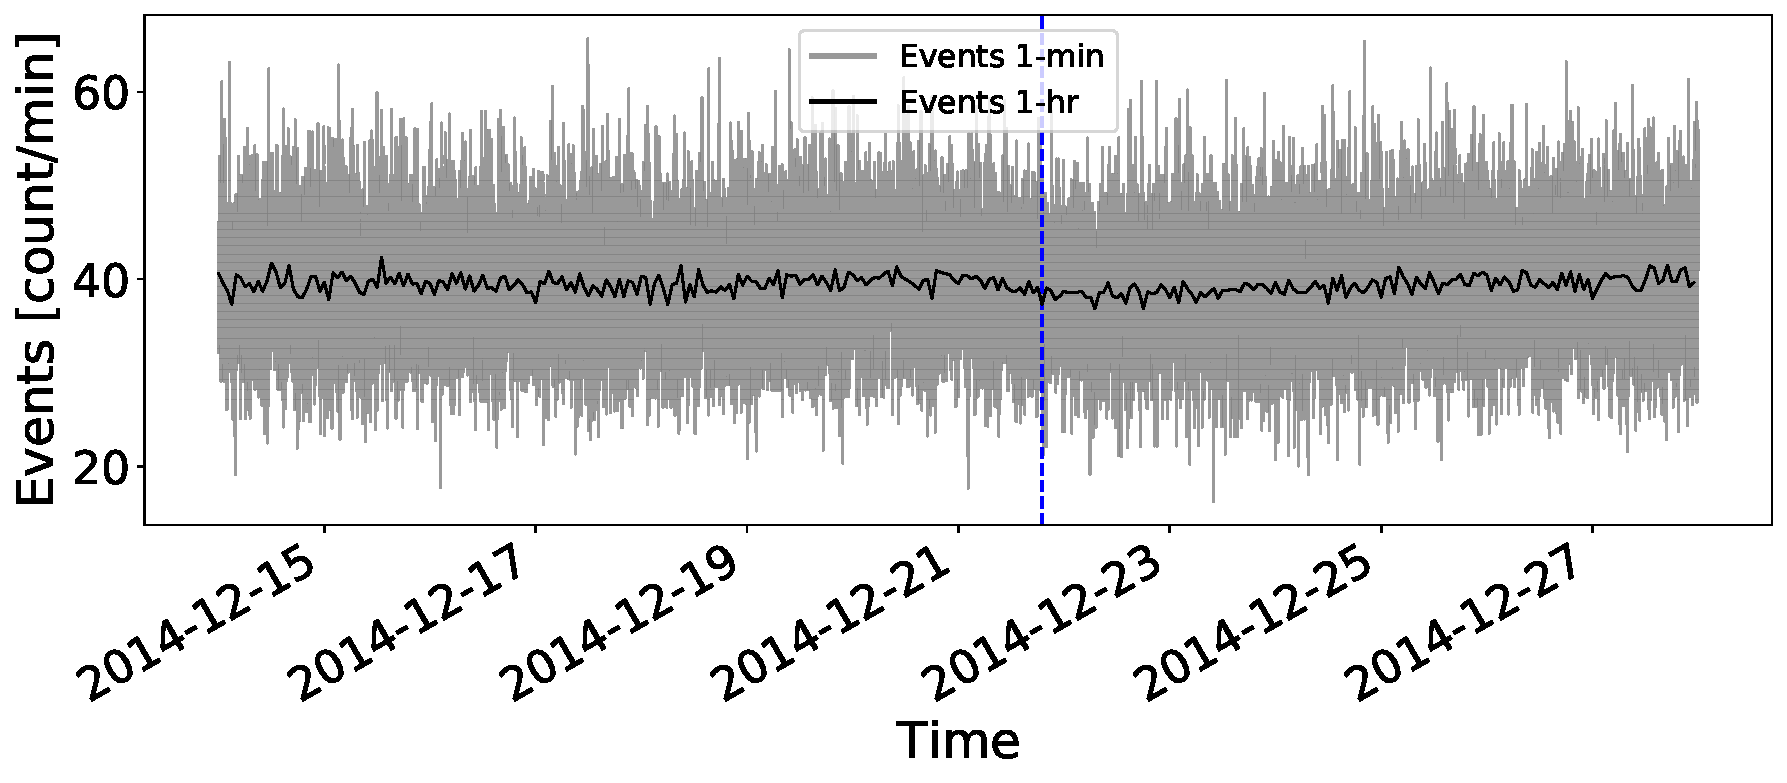
\includegraphics[width=0.65\columnwidth]{FD_201412_501_CORR.pdf}
	\caption{Atmospheric-corrected HiSPARC data for station 501 (Nikhef) around the epoch of the FD in December 2014. The plot shows the minute-averaged (grey) and hourly-averaged (black) trigger events between detectors within the station. The vertical blue, dashed line depicts the approximate onset time of the FD. The units of time on the x-axis are, YYYY-MM-DD.}
	\label{fig:FD_201412_501_Pcorr}
\end{figure}


In Figure~\ref{fig:FD_201207_8001_Pcorr} there are no clear \gls{fd} observations in the corrected \gls{hisparc} data; however, in Figure~\ref{fig:FD_201412_501_Pcorr} there is a slight indication of a $\sim2\%$ decrease in the count rate at the epoch of the expected \gls{fd}. This suggests that after correcting the data for atmospheric effects, that \glspl{fd} on the order of $\sim 2\%$ might be observed by the \gls{hisparc} network.

Finally, the atmospheric-effects corrected observations of the two \glspl{fd} which occurred around \gls{gle} 72 is shown in Figure~\ref{fig:FD_GLE72_Pcorr}, showing the corrected events data and singles data for each of the individual detectors in the stations.

\begin{figure}[ht!]
	\centering
	\subfloat[HS 501 (Nikhef)]{
		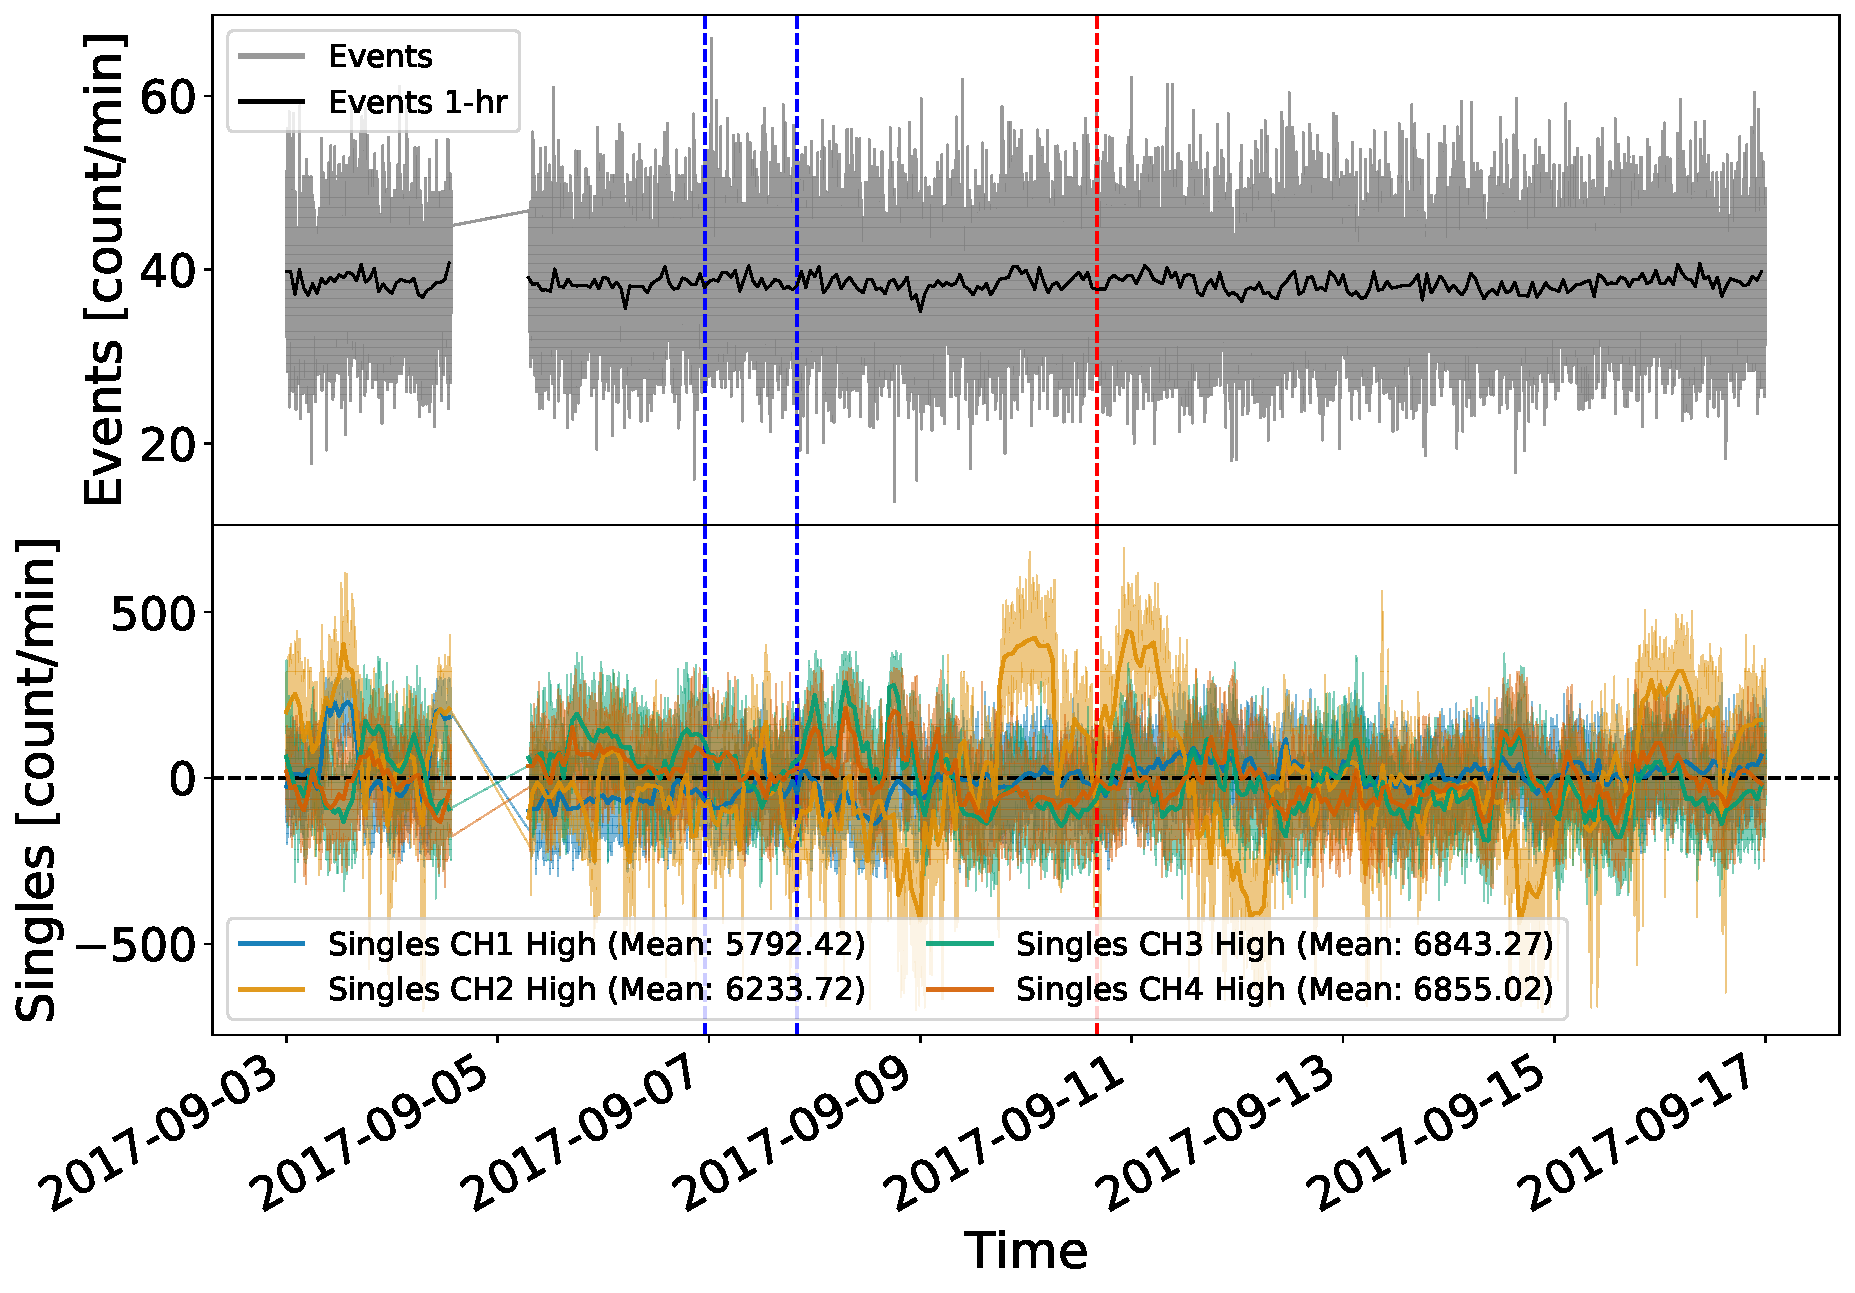
\includegraphics[width=0.48\columnwidth]{FD_GLE72_501_CORR.pdf}
		\label{fig:FD_GLE72_501_Pcorr}}
	%\qquad
	\subfloat[HS 203 (College Hageveld)]{
		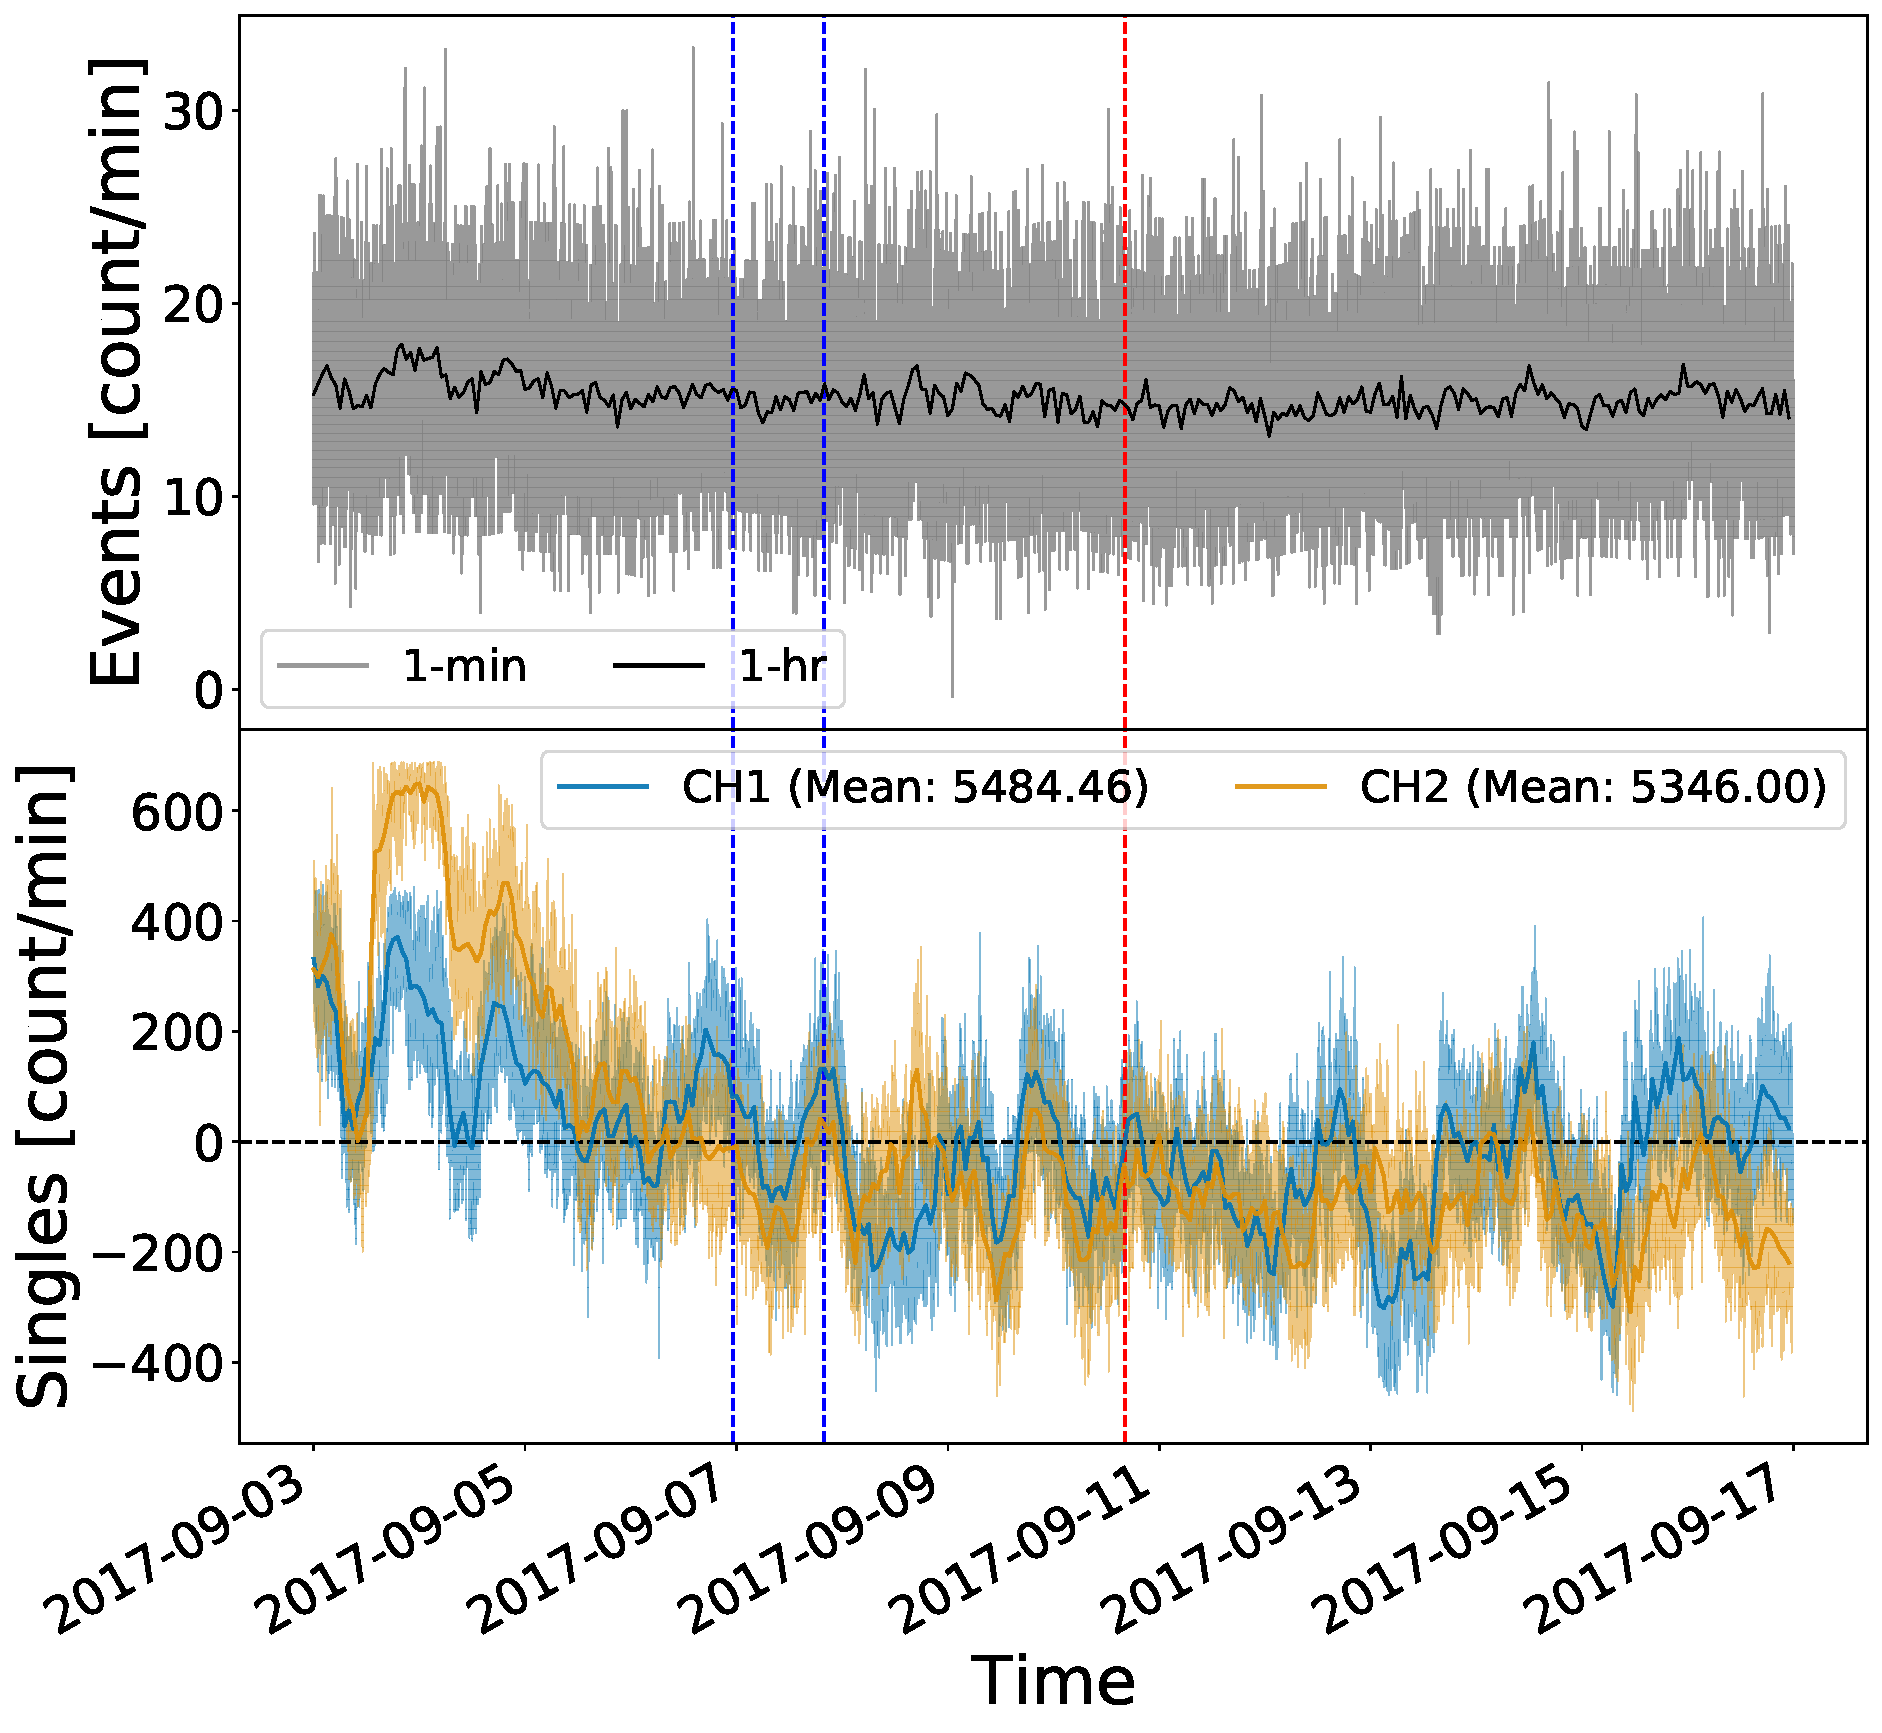
\includegraphics[width=0.48\columnwidth]{FD_GLE72_203_CORR.pdf}
		\label{fig:FD_GLE72_203_Pcorr}} \\
	
	
	\caption{Atmospheric-corrected HiSPARC data for 2 stations in an epoch where there were two FDs close to the onset of GLE 72. The top panel of each subplot shows the minute-averaged (grey) and hourly-averaged (black) trigger events. The bottom panel shows the minute- and hourly-averaged singles counts, mean-subtracted, for each individual detector (or signal channel, CH$n$) in the station. The vertical blue-dashed lines show the approximate onset-times of the FDs and the red-dashed line depicts the approximate onset-time of the GLE. The units of time on the x-axis are, YYYY-MM-DD.}
	\label{fig:FD_GLE72_Pcorr}
\end{figure}

There are no clear \glspl{fd} in Figure~\ref{fig:FD_GLE72_Pcorr}, and the singles plots demonstrate that the atmospheric corrections do no sufficiently remove all the signal excursions from the mean, and there remain large (up to $10\%$) deviations in the signals. One reason for this, particularly for the singles, is that the measured temperature is recorded in the atmosphere and not inside the roof boxes containing the \glspl{pmt}. The roof boxes are made of plastic and one would suspect the air temperature inside the boxes is different to the ambient atmospheric temperature measured nearby. In order to fully remove the effects of thermally induced count variations, we must record the more accurate temperatures of the \glspl{pmt} instead of just the atmospheric temperature.
% This highlights that although the method of atmospheric corrections does work, it does not always.



%%%%%%%%%%%%%%%%%%%%%%%%%%%%%%%%%%%%%%%%%%%%%%%%%%%%%%%%%%%%%%%%%%%%%
%%%%%%%%%%%%%%%%%%%%%%%%%%%%%%%%%%%%%%%%%%%%%%%%%%%%%%%%%%%%%%%%%%%%%
\section{Air Shower Simulations}\label{sec:CORSIKA}

%%%%%%%%%%%%%%%%%%%%%%%%%%%%%%%%%%%%%%%%%%%%%%%%%%%%%%%%%%%%%%%%%%%%%
\subsection{Motivation}

There is no evidence to suggest the \glspl{gle} were observed in the \gls{hisparc} data, even after correcting for atmospheric effects of pressure and temperature. This leads us to question whether it is possible to observe \glspl{gle} with the \gls{hisparc} detectors. In order to answer this, we needed to understand the muon flux at ground level and the scale of air shower muon footprints produced by \glspl{pcr}. To investigate this, simulations of air shower development were performed for a range of \glspl{pcr} energies for both primary protons and $\alpha$-particles. 

To simulate the \gls{cr} air shower development, the \gls{corsika} software was employed: a Monte Carlo programme providing detailed simulations of the evolution of air showers initiated by \glspl{pcr} through the atmosphere \citep{heck_extensive_2017}. The particles in the \gls{corsika} simulations are tracked through the atmosphere until they undergo interactions with atmospheric nuclei, decay due to their instability, or reach the ground level defined as the simulation terminator.

Proton and $\alpha$-particle initiated air showers were generated with energies ranging from $10^{9}$--$10^{20}$~eV, and $4\times10^{9}$--$10^{20}$~eV, respectively. In total $\sim 2\times10^5$ proton-initiated showers were simulated and $\sim 2\times10^5$ $\alpha$-particle-initiated air showers were simulated. Lists detailing the breakdown of \gls{pcr} energies and number of simulations is provided in Appendix~\ref{app:CORSIKA_sims}, along with a brief discussion of the settings chosen within the simulations.


%%%%%%%%%%%%%%%%%%%%%%%%%%%%%%%%%%%%%%%%%%%%%%%%%%%%%%%%%%%%%%%%%%%%%
\subsection{Air Shower Footprints}\label{sec:CORSIKA_footprint}

The average footprint of the muons at ground level, due to \glspl{pcr}, was calculated from the output of the \gls{corsika} simulations. This was achieved by taking the distribution of the number of muons at ground level at the end of the simulations as a function of their radial distance from the shower core, as this distance was provided as an output from the simulations. Multiple realisations of the air showers were simulated (see Table~\ref{tab:CORSIKA_proton_sims}). For a given \gls{pcr} energy, the mean distribution of radial footprints was calculated by averaging over all of the individual simulations. Figure~\ref{fig:shower_footprints} shows the radial distribution of muons at ground level for air showers induced by vertically incident protons and $\alpha$-particles.

In addition to the vertically induced air showers, we also repeated the simulations for air showers randomly selected from a uniform distribution of incident angles between 0$^\circ$ (vertical) and 70$^\circ$, to provide a simulation that is more physically representative of \glspl{cr} arriving from all directions. Radial distributions of muons were produced, similar to those in Figure~\ref{fig:shower_footprints}, but they are not shown here as the difference is not drastically different by-eye.

%[Discuss how distance between the HiSPARC station 2d/4d detectors will impact the ability to view certain PCR energies, and sets an lower limit on the energies observable in the standard trigger mode]

\begin{figure}[ht!]
	\centering
	\subfloat[Proton initiated air shower. \label{fig:p_footprint}]{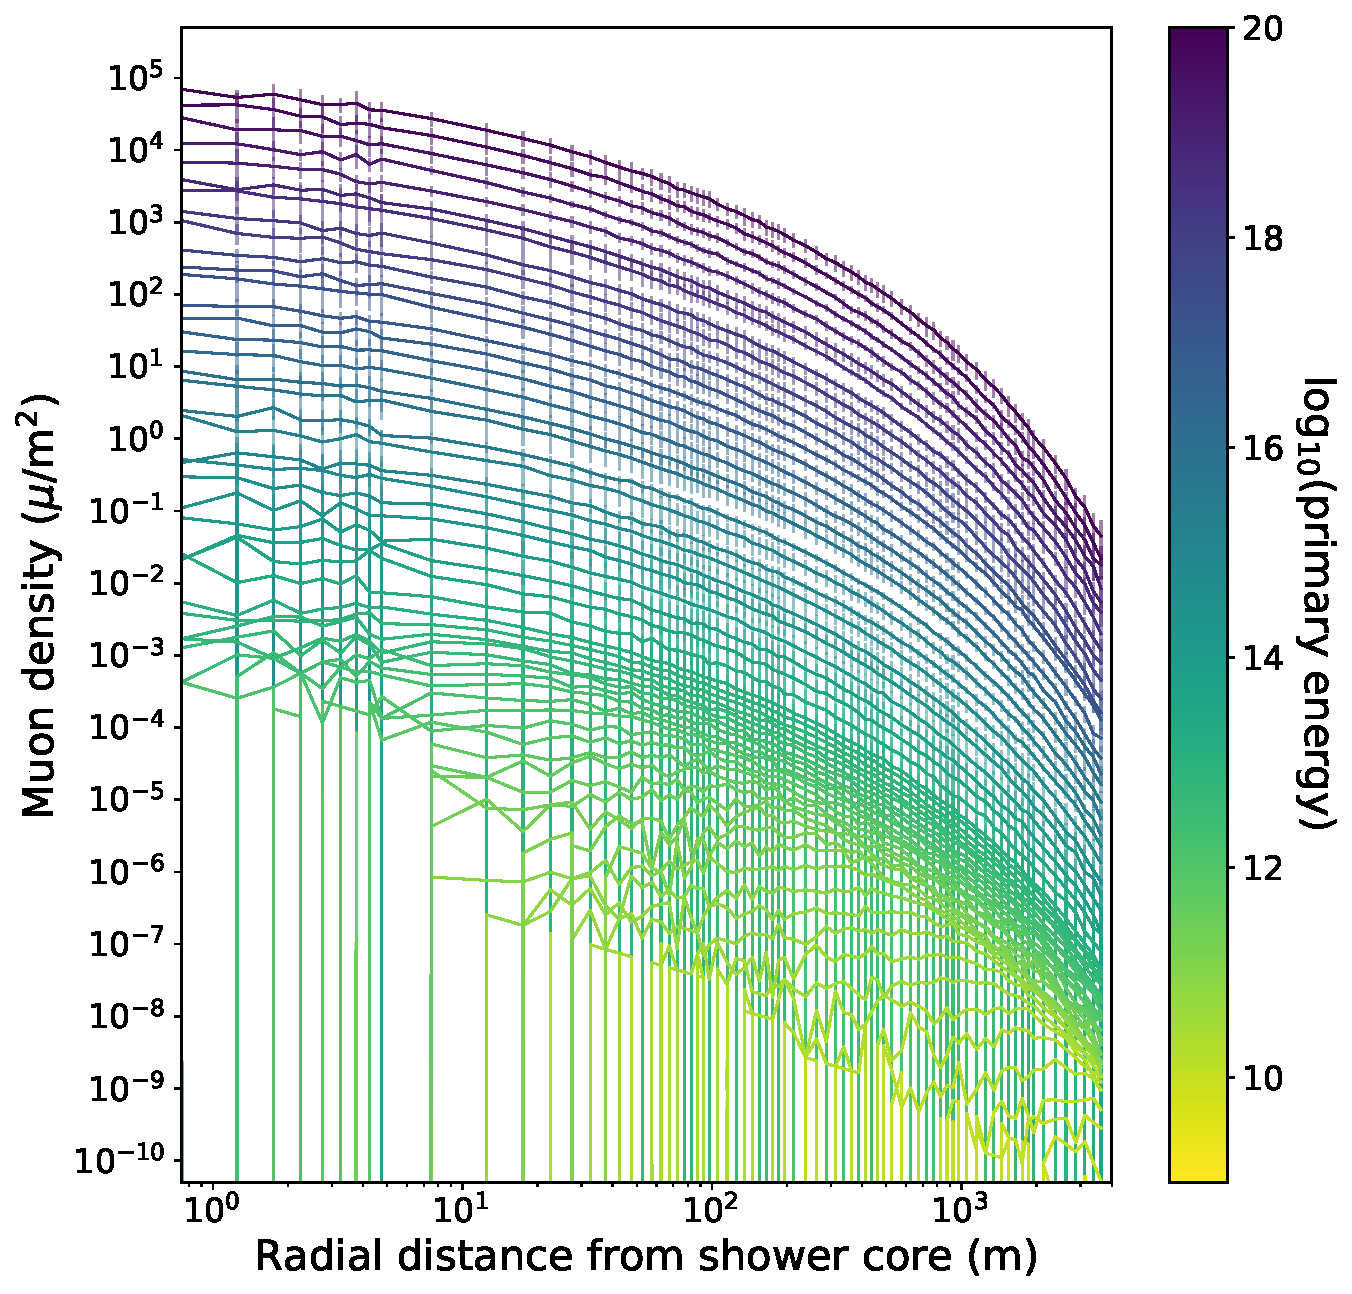
\includegraphics[width=0.47\columnwidth]{proton_footprint.pdf}} 
	\qquad
	\subfloat[$\alpha$-particle initiated air shower. \label{fig:a_footprint}]{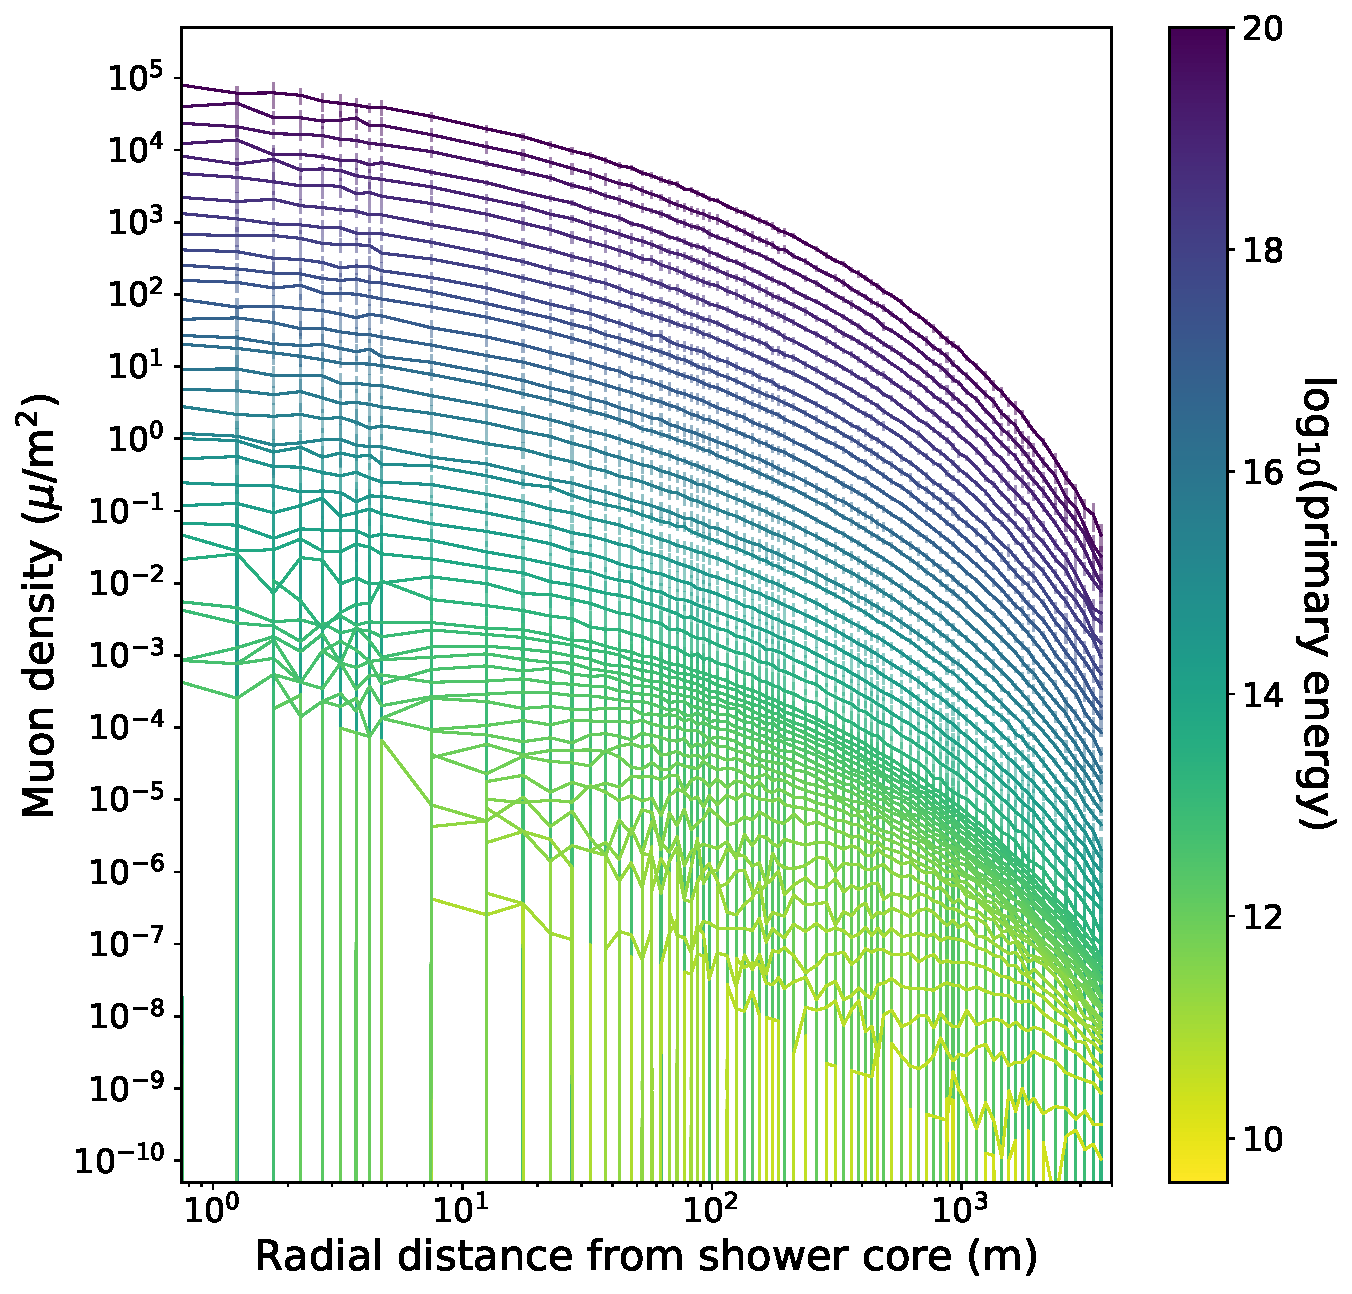
\includegraphics[width=0.47\columnwidth]{alpha_footprint.pdf}}
	\caption{Mean muon density footprints for (a) proton-initiated air showers and (b) $\alpha$-particle-initiated air showers with initial PCR trajectories with zenith angles $\theta=0^{\circ}$ and various PCR energies. The error bars given represent 1$\sigma$.} \label{fig:shower_footprints}
\end{figure}

The interpretation of Figure~\ref{fig:shower_footprints} provides an understanding of the minimum energy \glspl{pcr} observable by the \gls{hisparc} network. The typical separation between the detectors in a \gls{hisparc} station is $\sim 10$~m; however, the separation between detectors varies from station-to-station and can be up to as much as 20~m or as low as just a couple of metres. The simulations show, to trigger two \gls{hisparc} detectors separated by $\sim 10$~m by muons from the same shower, the density of the shower needs to be at least $\sim 0.005 \, \upmu \, \mathrm{m}^{-2}$, suggesting that \gls{hisparc} stations typically observe \glspl{pcr} with a minimum energy on the order of $\sim 10^{13} - 10^{14}$~eV, which agrees with what was found by \cite{van_dam_hisparc_2020}.

% we inferred that the variation in \gls{pcr} energy sampled varies marginally over this range of \gls{hisparc} detector separations. Furthermore it 

This helps to explain why the \glspl{gle} and \glspl{fd} were not observed in the \gls{hisparc} events data. The effects of \glspl{gle} and \glspl{fd} are more prominent at lower \gls{pcr} rigidities \citep{belov_solar_2005} and we showed here the air showers induced by these particles are not sufficient to induce an air shower that will trigger multiple detectors in a station. We see that lower energy \glspl{pcr} do not produce \glspl{eas}, but rather a very diffuse scattering of muons reach ground level. It is therefore clearer why we did not observe any \glspl{gle} in the events data, as the \gls{sep}-induced muons are insufficiently spread to trigger multiple detectors in coincidence. It would have been more likely to have observed \glspl{gle} in the singles data, as this only records the count rate of an individual detector, which has been shown to have a high muon-detection efficiency close to $100\%$ \citep{van_dam_hisparc_2020}. However, again the space weather events were not observed in the \gls{hisparc} singles data, which may be further explained by instead investigating the flux of muons at ground level.

%\begin{table}
%	\begin{center}
%		\caption{HS station minimum observable PCR energy}
%		\label{tab:footprints}
%		\begin{tabular}{l c c c}
%		\hline
%		{Station ID} & {Average separation (m)} & {Proton E$_{\mathrm{min}}$} & {$\alpha$-particle E$_{\mathrm{min}}$} \\
%		\hline
%		{501} & {11.2} & {} & {} \\
%		{14001} & {9.1} & {} & {} \\
%		{} & {} & {} & {} \\
%		\hline
%\end{tabular}
%\end{center}
%\end{table}


\subsection{Muon Flux}\label{sec:CORSIKA_flux}

Another output from the \gls{corsika} simulations was the energy of the muons that reach ground level. From the air shower simulations it was therefore possible to compute an estimate of the energy distribution of muons produced per \gls{pcr}. Figure~\ref{fig:shower_muons} shows the energy distribution of muons produced per primary \gls{pcr}, for air showers induced by vertically incident protons and $\alpha$-particles. The vertically incident air showers provide an upper boundary on the muon flux, but we also repeated the simulations for air showers randomly selected from a uniform distribution of incident angles between 0$^\circ$ (vertical) and 70$^\circ$, to provide a more physically representative flux. Similar plots were produced to those in Figure~\ref{fig:shower_muons}, but they are not shown here, as the difference is again not drastically different by-eye. 


\begin{figure}[ht!]
	\centering
	\subfloat[Proton initiated air shower. \label{fig:p_muons}]{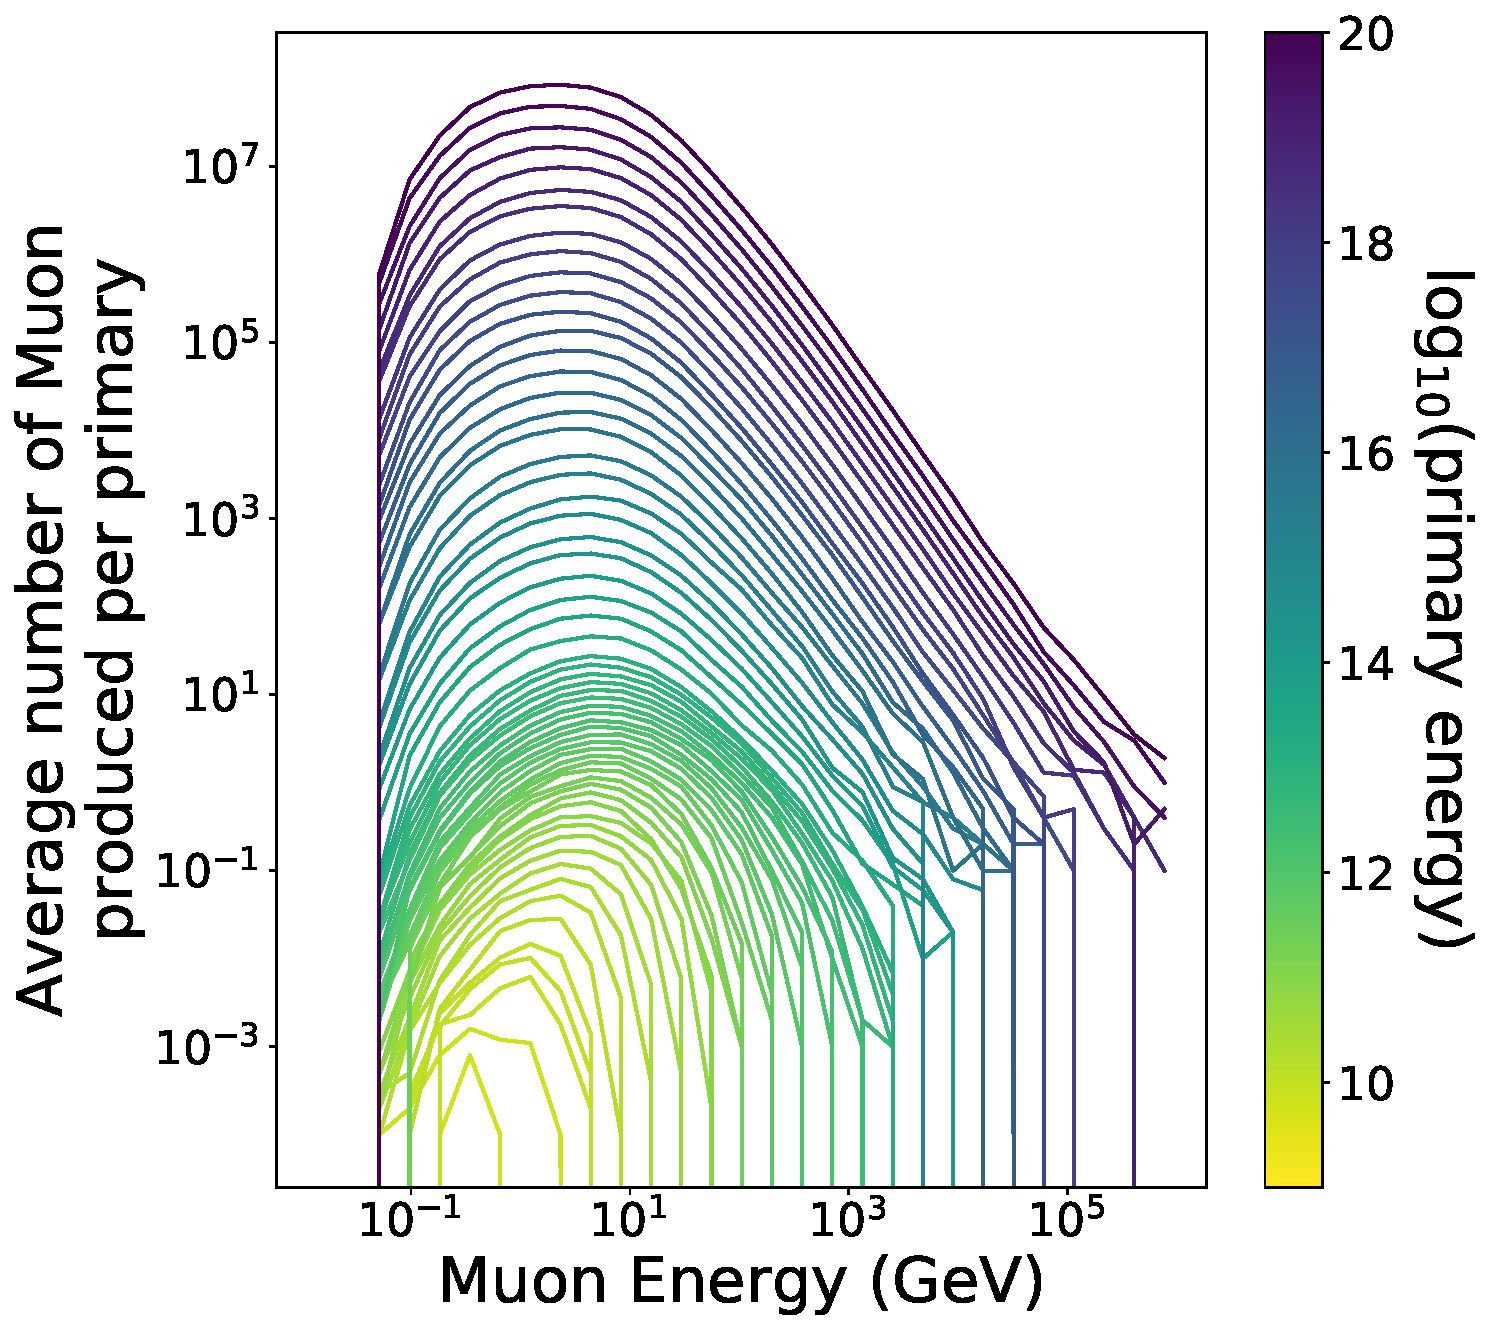
\includegraphics[width=0.47\columnwidth]{proton_muon_number.pdf}} 
	\qquad
	\subfloat[$\alpha$-particle initiated air shower. \label{fig:a_muons}]{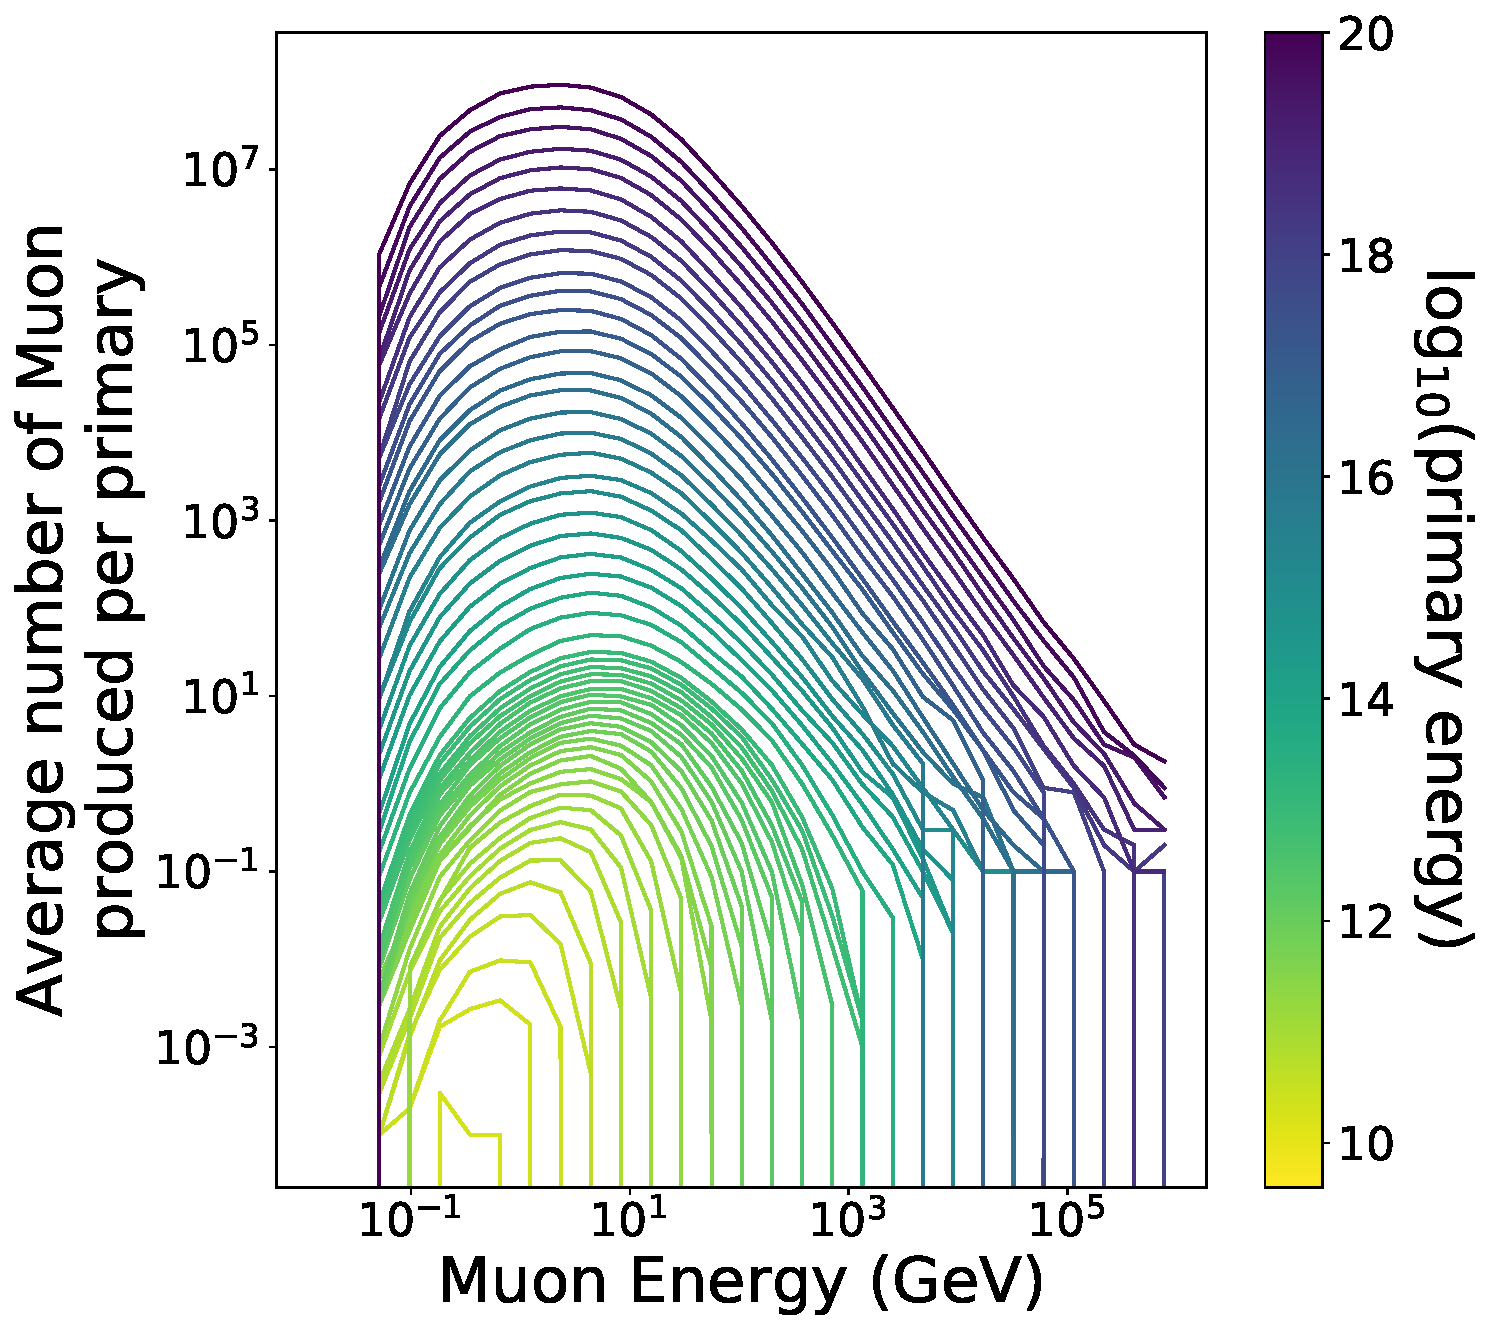
\includegraphics[width=0.47\columnwidth]{alpha_muon_number.pdf}}
	\caption{Mean number of muons produced at ground level by the PCR for (a) proton-initiated air showers and (b) $\alpha$-particle-initiated air showers, for various PCR energies.}
	\label{fig:shower_muons}
\end{figure}


We see from this analysis that \glspl{pcr} with an energy less than $\sim 10^{11}-10^{12}$~eV produce on the order of only one muon that reaches ground level, and below this energy it is rare that any muons arrive at ground level. Knowing the effects of \glspl{gle} and \glspl{fd} are more prominent at lower \gls{pcr} rigidities \citep{belov_solar_2005}, i.e. energies $<10^9$~eV, this helps explain why the space weather events were not observed in the \gls{hisparc} events data. The air showers induced by the lower rigidity \glspl{pcr} are insufficient to produce significant variations in the flux of the muons at ground level, thus we do not observe a variation from the typical \glspl{sep} that induce \glspl{gle}.

We also used the data from the simulations to estimate the total muon flux at ground level, based on the \gls{pcr} flux at the top of the atmosphere. We used a model for the \gls{gcr} flux at Solar Maximum \citep{corti_numerical_2019}, which utilised measurements from the \gls{ams} on-board the \gls{iss} to estimate the flux of \glspl{pcr} at the top of the atmosphere. Figure~\ref{fig:CORSIKA_muon_spectra} shows the computed differential flux of muons at ground level, based on the simulations of vertically incident \glspl{pcr} and those randomly simulated within a 70$^\circ$ acceptance cone. From Figure~\ref{fig:CORSIKA_muon_spectra}, we see that the ground-based flux is similar for both types of simulation performed. In both, the low-energy muon flux dominates and peaks at a muon energy of $\sim 1$~GeV.

% (do this by integrating under curve, using 70-degre half-angle cone for solid angle, and area of 0.5m2)
% i.e. in python doing doing:
% where df contains the alpha and proton diff fluxes
% v = scipy.integrate.simps(df_a_v[1]+df_p_v[1], df_a_v.index.values)
% sr = 4*np.pi*(np.sin(np.deg2rad(70/2)))**2
% area = 0.5
% rate_v = v*sr*area

%\begin{figure}[ht!]
%	\centering
%	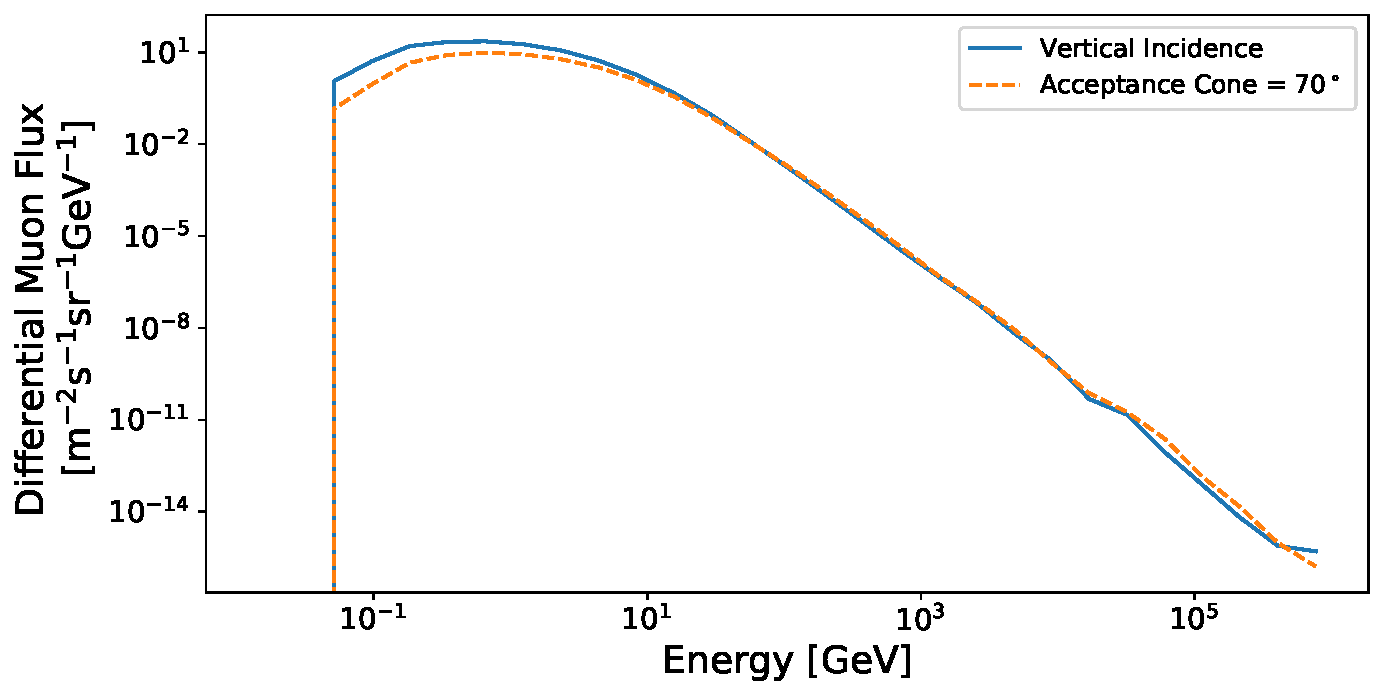
\includegraphics[width=\columnwidth]{CORSIKA_Muon_Diff_Flux_Comparison.pdf}
%	\caption{Muon differential flux computed using CORSIKA for vertically incident PCRs (solid, blue line) and for PCRs incident within an acceptance cone of $70^\circ$ (dashed, orange line).}
%	\label{fig:CORSIKA_muon_spectra}
%\end{figure}
\begin{figure}[ht!]
	\centering
	\subfloat[Differential muon flux]{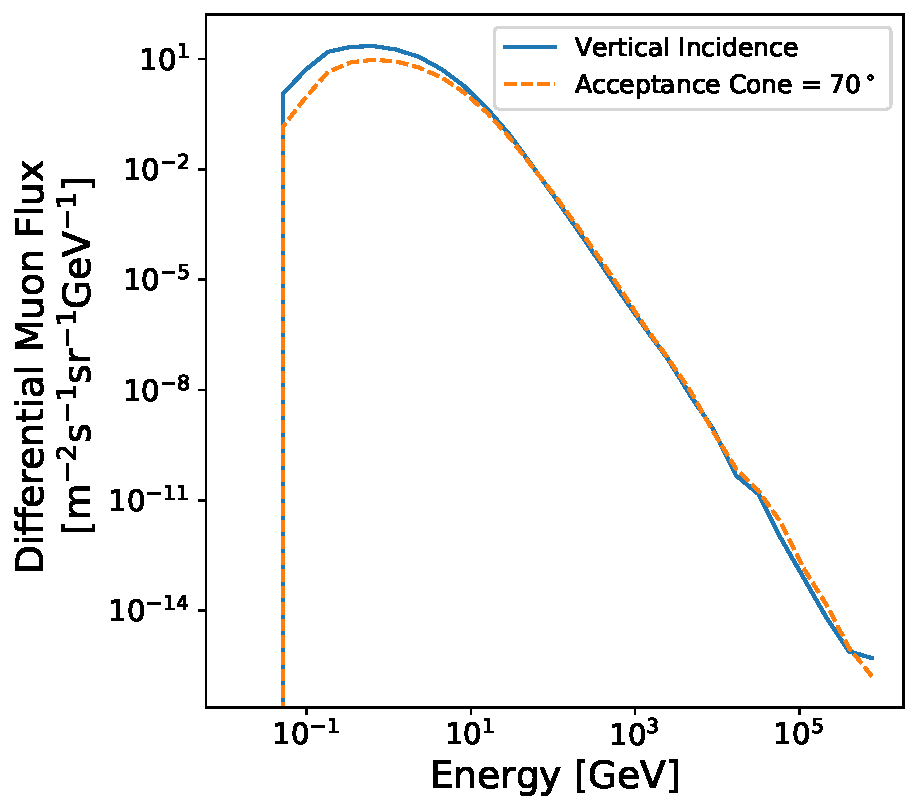
\includegraphics[width=0.47\columnwidth]{Total_Muon_Diff_Flux_Comparison.pdf}} 
	\qquad
	\subfloat[Muon flux through a single HiSPARC detector]{\includegraphics[width=0.47\columnwidth]{Total_Muon_Flux_Comparison.pdf}}
	\caption{Ground level muon spectra as computed in the CORSIKA simulations. (a) shows the differential muon flux at ground level; (b) shows the muon flux through a single HiSPARC detector. In both plots the solid, blue line shows the simulations using vertically incident PCRs, and the dashed, orange line shows the simulations using PCRs incident within a cone of $70^{\circ}$.}
	\label{fig:CORSIKA_muon_spectra}
\end{figure}



The calculated spectra were used to determine the expected rate of muons passing through a single \gls{hisparc} detector. We computed the rates: $\sim 85 \, \upmu/\mathrm{s}$ (for non-vertical, i.e. $70^\circ$ acceptance cone simulations), and $160 \, \upmu/\mathrm{s}$ (for vertical simulations). These rates are comparable to the generally accepted, average ground level muon flux on the order of $\sim 70$~$\mathrm{m}^{-2}\,\mathrm{s}^{-1}\,\mathrm{sr}^{-1}$ \citep{cecchini_cosmic_2000, blackmore_terrestrial_2015, pereira_ground_2020, particle_data_group_review_2020}, or 1--2~$\upmu\,\mathrm{cm}^{-2}\,\mathrm{min}^{-1}$ \citep{particle_data_group_review_2020}, which imply a rate of $\sim140 \, \upmu/\mathrm{s}$. 
%$85.365 \, \upmu/\mathrm{s}$ and $156.924 \, \upmu/\mathrm{s}$ ... $\sim 1$ per cm$^2$ per second

To understand, from the \gls{corsika} simulations, how the muon count rate changes during a \gls{gle}, the \gls{pcr} spectrum during the space weather events is needed. Unfortunately this information was not so easily acquired; however, there is a tool which provided muon fluxes based on the \gls{gcr} spectrum and also \gls{gle} spectra, which is described in the next section.



\subsection{Muon Flux From MAIRE}\label{sec:MAIRE_flux}

As a further comparison, to investigate how the muon flux varied during \glspl{gle} we used the online \gls{maire} tool to compute the muon spectrum at ground level \citep{dyer_calculations_2003, lei_atmospheric_2004}. \gls{maire} allows the computation of the secondary particle spectra in the atmosphere, caused by \glspl{sep}, including the ground level neutron and muon fluxes. \gls{maire} has an advantage of also having the \gls{pcr} spectra for a number of \glspl{gle} built-in; however, they are for the strongest \glspl{gle} to-date, which we need to take into consideration, so we do not bias our inferences. The \gls{gle} events that can be simulated within the \gls{maire} tool are detailed in Table~\ref{tab:MAIRE_GLEs}, also providing an estimate for the maximum increase in count rate, as observed in the \gls{nmdb}, as a reference.

\begin{table}[ht!]
	\begin{center}
		\caption{The seven GLEs where MAIRE muon spectra were available, and the maximum observed increase in the neutron flux in the NMDB and the station where the increase was observed.}
		\label{tab:MAIRE_GLEs}
		\begin{tabular}{l c c c c c}
			\hline
			%			&  & \multicolumn{2}{c}{\bf \% Change} \\
			{\bf GLE} & {\bf Date} & {\bf Max. \% change (station)} \\
			\hline
			5  & 23/02/1956 & $\sim 5100\%$ (Leeds) \\
			42 & 29/29/1989 & $\sim 340\%$ (Calgary) \\
			43 & 19/10/1989 & $\sim 90\%$ (South Pole) \\
			44 & 22/10/1989 & $\sim 190\%$ (McMurdo) \\
			45 & 24/10/1989 & $\sim 200\%$ (South Pole) \\
			59 & 14/07/2000 & $\sim 60\%$ (South Pole) \\
			60 & 15/04/2001 & $\sim 220\%$ (South Pole) \\
			\hline
		\end{tabular}
	\end{center}
\end{table}

The \glspl{gle} incorporated in the \gls{maire} tool predate the existence of the \gls{hisparc} network; as a result, the simulations are not directly informative on the \glspl{gle} we were investigating in Table~\ref{tab:space_weather_events}. Nevertheless, the \gls{maire} simulations helped in our understanding of whether it was possible to observe a \gls{gle} using data acquired by the \gls{hisparc} network.


We first used the \gls{maire} tool to simulate the spectra for the background \glspl{gcr} and the seven \glspl{gle} at the Nikhef (501) \gls{hisparc} station. Figure~\ref{fig:MAIRE_muon_spectra} shows the muon spectra for the \gls{gcr} spectrum at solar minimum, and the additional muon spectrum for seven of the largest \glspl{gle} to date (which are additive to the \gls{gcr} spectrum).


\begin{figure}[ht!]
	\centering
	\subfloat[Separate GCR and GLE Muon Spectra]{\includegraphics[width=0.47\columnwidth]{Muon_Diff_Flux.pdf}} 
	\qquad
	\subfloat[Sum of GCR and GLE Muon Spectra]{\includegraphics[width=0.47\columnwidth]{Muon_Diff_Flux_Additive.pdf}}
	\caption{Plots of the calculated MAIRE muon spectra for different incident PCR spectra. Blue and orange lines show muon spectra calculated for the incident GCR spectra during solar minimum and maximum, respectively. The other coloured lines show the computed muon spectra for the incident GLE spectra. (a) shows the individual muon spectra for GCRs and GLEs; (b) shows the combined muon spectra for the GCR at solar maximum and the GLEs.}
	\label{fig:MAIRE_muon_spectra}
\end{figure}


The \gls{gcr}-induced muon spectrum in Figure~\ref{fig:MAIRE_muon_spectra} roughly agrees with that computed using \gls{corsika}, which gave us confidence in the results of both simulations. We can see that the effect on the muon spectrum drastically varies for the seven \glspl{gle}, with \gls{gle} 5 clearly the largest event.

Prior to inferring any conclusions about the \gls{gle}-induced muon spectra at the \gls{hisparc} stations, as the \gls{maire} tool provides the neutron flux, we verified the accuracy of the \gls{maire} results by comparing the observed increases in \gls{nm} count rates to those predicted by \gls{maire}. To reduce any effects of strong anisotropy, when comparing to \gls{hisparc}, we chose to analyse the \gls{nm} count rate at a mid-latitude station, Kiel, which is located in Germany and is one of the nearest \gls{nm} to the \gls{hisparc} network, at $\sim 825$~km away. The properties of the Kiel station are: $R_C$=2.36~GV, Altitude=54~m, Latitude=$54.34^{\circ}$N, Longitude=$10.12^{\circ}$E \citep{nmdb_nmdb_nodate}; these are similar to the properties of the \gls{hisparc} stations.

Table~\ref{tab:KIEL_GLEs} shows a comparison between the observed neutron count increase, measured using data from the \gls{nmdb}, and the increases predicted by \gls{maire}. The Kiel \gls{nm} station was not online in 1956, during \gls{gle} 5, therefore this event has been omitted from these results. The \gls{maire} increases were calculated by comparing the integrated \gls{gle} flux to the integrated background \gls{gcr} flux at that epoch, including the effects of the disturbances in the Earth's magnetic field from the planetary K-index ($K_p$) \citep{bartels_three-hour-range_1939}. The muon count rate increases predicted by \gls{maire} are also shown in Table~\ref{tab:KIEL_GLEs}, for comparison.

\vspace{1em}

\begin{table}[ht!]
	\begin{center}
		\caption{Observed and predicted increases in the CR count rates at the Kiel NM station, with rows ordered by the observed NM magnitude. The observed neutron increases use data from the NMDB, where the errors are the measurement uncertainty from the 5-minute averaged data. The predicted data for the neutrons and muons are from the MAIRE simulations. The ratio column provides a conversion factor from the MAIRE predicted neutron increases compared to those observed. The fraction column shows the proportion of the MAIRE predicted muon increase compared to the MAIRE predicted neutron increase. The rows are ordered by the observed NM magnitude.}
		\label{tab:KIEL_GLEs}
		\begin{tabular}{l c c c | c c}
			\hline
			&  \multicolumn{2}{c}{\bf Neutron Increase} & & {\bf Muons Increase} & \\
			{\bf GLE} & {\bf Observed} & {\bf Predicted} & {\bf Ratio} & {\bf Predicted} & {\bf Fraction}\\ 
			\hline
			42 & $\sim~160\pm5$~\% & 88.7\% & 1.80 & 3.98\% & 4.45\% \\
			45  & $\sim~45\pm2$~\% & 67.9\% & 0.66 & 0.817\% & 1.20\% \\
			60 & $\sim~24\pm2$~\% & 18.8\% & 1.28 & 0.0814\% & 0.43\% \\
			43 & $\sim~19\pm1$~\% & 59.6\% & 0.32 & 0.790\% & 1.32\% \\
			59 & $\sim~8\pm1$~\% & 6.1\% & 1.32 & 0.00906\% & 0.15\% \\
			44  & $\sim~6\pm1$~\% & 2.6\% & 2.30 & 0.00376\% & 0.14\% \\
			5 & - & - & - & - & - \\
			\hline
		\end{tabular}
	\end{center}
\end{table}

We can see from Table~\ref{tab:KIEL_GLEs} that there is a stark contrast between the observed \gls{nm} increase and that predicted by \gls{maire}. One possible cause is inaccuracy in the predictions; however, this is unlikely as \citet{lei_atmospheric_2004} have shown the verification of their results versus observations, providing that \gls{maire} is robust. More likely, the difference is due to the anisotropy of the \glspl{cr} initiating the \glspl{gle}, as \gls{maire} does not account for anisotropy in the simulations \citep{dyer_calculations_2003, lei_atmospheric_2004}. It is also possible that there is an unknown factor that causes this discrepancy, but we cannot postulate on this. The ratio column gives a factor to convert from the \gls{maire} predicted increase to the \gls{nmdb} observed increase, assuming that there are no other physical reasons why the predictions and observations differ. We assumed this could be used as a calibration factor, to ensure agreement between the \gls{maire} predictions and the observed data.

The ranked ordering of the events in Table~\ref{tab:KIEL_GLEs}, from strongest to weakest \glspl{gle}, shows the order of observed Kiel data and \gls{maire}-predicted data are in good agreement, suggesting that despite an incorrect magnitude of the increase, there is agreement between the two data sets. This supports the use of the calibration factor. In addition, comparing the fraction of the predicted muon increase to the predicted neutron increase, shown in Table~\ref{tab:KIEL_GLEs}, we see the significantly smaller prediction for the muons. We know this is due to the energy spectrum of the \glspl{pcr}, but the values in Table~\ref{tab:KIEL_GLEs} provide a quantitative estimate of this and serves as further evidence to show that we may be unable to observe weaker \glspl{gle} with the \gls{hisparc} network. We see similarly small predictions for the \gls{hisparc} stations, which are shown in Table~\ref{tab:MAIRE_raw_muons}. There is good agreement in the predicted muon increase at the Kiel and \gls{hisparc} stations. However, this agreement seems to depend on size of increase, with the weaker events showing less good relative agreement; this is down to the error in the predicted increase for such low-magnitude \glspl{gle}.

\vspace{1em}

\begin{table}[ht!]
	\begin{center}
		\caption{The MAIRE predicted increase in the muon flux at Kiel and two HiSPARC stations. The rows are ordered by the observed NM magnitude from Table~\ref{tab:KIEL_GLEs}.}
		\label{tab:MAIRE_raw_muons}
		\begin{tabular}{l c c c c c}
			\hline
			&  \multicolumn{3}{c}{\bf Predicted Muon Increase} \\
			{\bf GLE} & {\bf Kiel} & {\bf HS 501} & {\bf HS 14001} \\
			\hline
			42 & 3.98\%    & 3.97\%    & 4.06\%  \\
			45 & 0.817\%    & 0.798\%    & 0.847\%  \\
			60 & 0.0814\%   & 0.0768\%   & 0.0808\%  \\
			43 & 0.790\%    & 0.774\%    & 0.817\%  \\
			59 & 0.00906\%  & 0.00563\%  & 0.00683\%  \\
			44 & 0.00376\% & 0.00241\% & 0.00305\%  \\
			5 & - & - & - \\
			\hline
		\end{tabular}
	\end{center}
\end{table}


As the ratio column in Table~\ref{tab:KIEL_GLEs} provided us with a calibration to recover the observed increase in neutron counts from those predicted in the \gls{maire} simulations, we used the assumption that the calibration factor may also be applied to the predicted increase in the muon counts, to recover the `true' values. This assumed that both detectors only observe particles from \glspl{as} (i.e. from the `sky') and we do not observe regenerative particles.

In particular, we also intended to apply this calibration to the predicted magnitudes for the \gls{hisparc} stations. To test that this was acceptable, and verify that the \gls{hisparc} stations are sufficiently close to Kiel such that the deviation in the prediction is minimal, we investigated the dependence of the \gls{gle} magnitude on the latitude, longitude, and altitude of the location of the detector. The results of the simulations are shown in Figure~\ref{fig:GLE42_MAIRE_test}. This plot shows the predicted increase in muons during \gls{gle} 42 when varying geographical parameters in the simulations. The blue square, orange up-triangle, and green down-triangle show the predicted magnitude at the location of the Kiel \gls{nm} station, and \gls{hisparc} stations 501 and 14001, respectively. The black circles represent the predicted magnitude when changing a single property (either latitude, longitude, or altitude) of the Kiel station during the simulations. The top panel in Figure~\ref{fig:GLE42_MAIRE_test} shows the relationship with latitude, the middle panel shows the relationship with longitude, and the bottom panel shows the relationship with altitude. %This conversion is shown in Table~\ref{tab:MAIRE_muons}. 


\begin{figure}[ht!]
	\centering
	\includegraphics[width=0.9\columnwidth]{GLE42_variation_plot.pdf}
	\caption{Shows the relationship between the predicted magnitude of GLE 42 and geographical location. Blue square shows the predicted muon increase at the Kiel station, orange up-triangle for HiSPARC station 501 (Nikhef), and green down-triangle for HiSPARC stations 14001 (University of Birmingham). The black points show the results when varying one property of the Kiel simulations, in the top panel we vary latitude; middle panel the variation with longitude; the bottom panel shows the variation with altitude.}
	\label{fig:GLE42_MAIRE_test}
\end{figure}


From Figure~\ref{fig:GLE42_MAIRE_test}, we found that the largest change in the predicted \gls{gle} magnitude occurred as a result of varying the latitude, which is expected due to the change in rigidity cut-off. The variation with longitude was marginal because \gls{maire} does not account for anisotropy and the variation with altitude was notable. However, the important result from Figure~\ref{fig:GLE42_MAIRE_test} was the good agreement in the predicted muon increase between Kiel and the \gls{hisparc} stations, and the biggest variation was for the station in Birmingham, which was solely due to the altitude difference, according to the lower panel in Figure~\ref{fig:GLE42_MAIRE_test}. The results show that there is a lack of variance in the model predictions over the geographical scale between all three locations, hence we were confident enough to apply the same neutron-based calibration factor to all the muon predictions.

%However, this agreement seems to depend on size of increase, with the weaker events showing less good relative agreement. We believe this is down to the error in the predicted increase for such low-magnitude \glspl{gle}
%%%---
%Kiel and these two HS stations are physically close (similar geographic locations, comparable altitudes, therefore it is reasonable to expect similar muon observations at these locations. MAIRE predictions bear this out; values (not shown) are similar at all three locations. Based on both of these points, we attempt to use the neutron-based calibration factor to correct the muon predictions from MAIRE

Based on the results in Figure~\ref{fig:GLE42_MAIRE_test} we used the neutron-based calibration factor to correct the muon predictions from \gls{maire} for the muon count rate at Kiel and the two \gls{hisparc} stations, and the calibrated values are given in Table~\ref{tab:MAIRE_muons}. These values effectively represent a zeroth- or first-order approach to estimating the muon increase that would be observed for these \glspl{gle} with the information we have available. The calculations relied on the assumption that the application of the calibration factor was acceptable, and that anisotropy does not have a significant effect on the increase observed between the Kiel \gls{nm} station and the \gls{hisparc} stations in the Netherlands and the UK. In addition, we cannot quantify the uncertainty in the \gls{maire} simulations, but assume that the uncertainty is small. \gls{gle} 5 has been omitted from these results as the Kiel station was not online then, so we cannot calibrate the \gls{maire} predictions. %The predicted count rates, adjusted for the factors in Table~\ref{tab:KIEL_GLEs}, are shown in Table~\ref{tab:MAIRE_muons}. Again, \gls{gle} 5 has been omitted from these results as the Kiel station was not online then, so we cannot calibrate the \gls{maire} predictions.


\begin{table}[ht!]
	\begin{center}
		\caption{The MAIRE predicted increase in the muon flux, adjusted for the calibration factor between observed and predicted neutron increases at the Kiel station, in Table~\ref{tab:KIEL_GLEs}. The rows are ordered by the observed NM magnitude from Table~\ref{tab:KIEL_GLEs}.}
		\label{tab:MAIRE_muons}
		\begin{tabular}{l c c c c c}
			\hline
			&  \multicolumn{3}{c}{\bf Calibrated Muon Increase} \\
			{\bf GLE} & {\bf Kiel} & {\bf HS 501} & {\bf HS 14001} \\
			\hline
			42 & 7.18\%    & 7.15\%    & 7.33\%  \\
			45 & 1.47\%    & 1.44\%    & 1.53\%  \\
			60 & 0.147\%   & 0.139\%   & 0.146\%  \\
			43 & 1.42\%    & 1.40\%    & 1.47\%  \\
			59 & 0.0163\%  & 0.0102\%  & 0.0123\%  \\
			44 & 0.00678\% & 0.00435\% & 0.00550\%  \\
			5 & - & - & - \\
			\hline
		\end{tabular}
	\end{center}
\end{table}


%The predicted increase in the muon count rates, calculated using the \gls{maire} simulations, for the \gls{nm} station and the \gls{hisparc} stations, in both the Netherlands and the UK, are in near-agreement. Assuming the effects of anisotropy are small, this suggests that the predicted spectra at the \gls{hisparc} stations (adjusted for the calibration factor) are representative of the approximate increase one would expect to observe.

The effect of the \glspl{gle} shows only a small increase in the muon count rate, and for most of the events induces an increase of $< 2 \%$ in the ground-level muon flux. Furthermore, for the weaker, more frequent standard of \glspl{gle} an increase of $\ll 1\%$ was predicted. The exception in these events is \gls{gle} 42. We expect that we would have seen the increase in the \gls{hisparc} data for \gls{gle} 42, but it pre-dates the \gls{hisparc} project and thus it cannot be verified. We expect the same would have been true also for \gls{gle} 5, but we do not have the Kiel data to form the calibration, to predict the increase. \gls{gle} 5 was an exceptionally large event, for which we have not seen anything similar in over half a decade. Such events are rare, and we expect that the energies involved would have shown a significant increase in the \gls{hisparc} count rate.

These simulations, combined with the values given in Table~\ref{tab:space_weather_events}, suggest that we would have expected an increase in the muon spectrum of $< 0.1\%$ for both \gls{gle} 71 and 72, which rules their observation with \gls{hisparc} as extremely unlikely and helps explain why we were unable to observe them in the preceding investigation in this chapter. \gls{gle} 70 induced a larger increase in the Kiel neutron counts on the order of $\sim 30\%$, but comparing this with similar values in Table~\ref{tab:KIEL_GLEs} and Table~\ref{tab:MAIRE_muons} suggests we would still only expect an increase in the \gls{hisparc} count rate between $\sim 0.1 - 2 \%$. In each of these cases it is very unlikely that we would have observed the \glspl{gle} using the \gls{hisparc} network.

From these results we must therefore conclude that the \gls{hisparc} network, in its current state, is unable to observe the more abundant standard of \glspl{gle}, but it is likely able to observe the rare, highly energetic events, such as that seen in 1956 leading to \gls{gle} 5.



%%%%%%%%%%%%%%%%%%%%%%%%%%%%%%%%%%%%%%%%%%%%%%%%%%%%%%%%%%%%%%%%%%%%%%
%%%%%%%%%%%%%%%%%%%%%%%%%%%%%%%%%%%%%%%%%%%%%%%%%%%%%%%%%%%%%%%%%%%%%%
%
%\section{Discussion}\label{sec:HS_discussion}




%%%%%%%%%%%%%%%%%%%%%%%%%%%%%%%%%%%%%%%%%%%%%%%%%%%%%%%%%%%%%%%%%%%%%
%%%%%%%%%%%%%%%%%%%%%%%%%%%%%%%%%%%%%%%%%%%%%%%%%%%%%%%%%%%%%%%%%%%%%
\section{Conclusion}\label{sec:HS_conclusion}

We have presented a feasibility study on using the existing \gls{hisparc} network of muon detectors to monitor space weather events. This was achieved through calculating the observing properties of \gls{hisparc} stations, investigating the presence of space weather signatures in the existing data for five \gls{hisparc} stations, both in their raw form and after performing corrections for atmospheric effects, and by performing cosmic ray air shower simulations.

Using simulations of the interactions of \glspl{cr} with the Earth's magnetosphere in the PLANETOCOSMICS tool, we were able to calculate the rigidty cut-off and \glspl{avd} of the \gls{hisparc} stations. We showed that the rigitidy cut-off limits the \glspl{pcr} to particles with energies on the order of and above $\sim 10^9$~eV. The \glspl{avd} were useful in demonstrating that the observable, lower rigidity \glspl{pcr} are deflected significantly by the Earth's magnetosphere and we may observe solar eruptive events when the station is not pointing in a direction in-line with the Sun.

In the raw \gls{hisparc} data we found that we were unable to clearly detect signatures of the \glspl{fd} or \glspl{gle} that have occurred over the lifetime of the \gls{hisparc} network. It was observed that a major obstructing factor was due to atmospheric effects causing additional variations in the data. Using a linear relationship between the logarithm of the normalised \gls{cr} counts against both the zero-centred pressure and temperature, the atmospheric effects were corrected for in the data.

After the correction of the atmospheric effects, when investigating the corrected \gls{hisparc} data we found that we were still unable to observe any \glspl{gle}. The same was true for most of the \glspl{fd}; however, we do speculate that we were able to observe a signature of the \gls{fd} in December 2014. 

A further study was conducted to understand the flux of muons at ground level, and in particular how the flux varied during \glspl{gle}. Using Monte Carlo simulations of particle transport through the atmosphere for incident \glspl{pcr}, with \gls{corsika}, were were able to interrogate the number and radial distribution of muons arriving at ground-level per \gls{pcr}. This highlighted that the flux of muons is very low for \glspl{pcr} with energies less than, or in the region of, the rigidity cut-off of the \gls{hisparc} stations. This analysis therefore showed that any increase in the \gls{cr} count from \glspl{gle} would likely be very low, due to the diffuse nature of the air showers induced by the low-energy \glspl{pcr} that primarily make up the \gls{gle}-inducing \gls{sep} spectra. To observe events with \gls{hisparc} we are excluded to only the most energetic events that are sufficient to produces large muons \glspl{as}.

Expanding on this analysis, a comparative study was conducted using the \gls{maire} tool. This allowed us to directly predict the increase in \gls{cr} counts based on simulations of incident \glspl{pcr}, comparing the output muon flux from \glspl{gcr} and \glspl{gle}. A calibration was necessary to ensure that the \gls{maire} predictions were consistent with the \gls{nmdb} observations; however, upon applying this calibration, we were able to show that the predicted increase in the muon count rate was significantly lower than the neutron count rate, for each of the six \glspl{gle} studied. We assumed that it was acceptable to apply to same calibration to the predicted values for two \gls{hisparc} stations, which was validated with simulations across various latitudes, longitudes, and altitudes. This led us to conclude that the \gls{hisparc} network is only capable of observing the most energetic \glspl{gle}, which occur less frequently than their lower energy equivalents.

We leave the reader with the following points:

\begin{enumerate}
	\item{The rigidity cut-off and \glspl{avd} of the \gls{hisparc} stations were calculated using \gls{pcr} transport simulations. We found the \gls{hisparc} stations generally have a cut-off rigidity in the range, $R_C \sim 3.0 - 3.5$~GV, setting a limit on the \glspl{pcr} observable on the order of $\sim 10^9$~eV. The asymptotic viewing directions for the \gls{hisparc} stations are close to equatorial for low rigidity \glspl{pcr}, between $\pm 20^{\circ}$ in latitude, and tend towards the station's zenith for rigidities greater than 20~GV.}
		
	\item{Investigations of the raw and atmospheric corrected data showed no signatures of \glspl{gle} in the \gls{hisparc} data. We propose that one \gls{fd} was observed as a $\sim 2\%$ decrease in the atmospheric corrected data; however, none of the other events were observed in the \gls{hisparc} data.}
	
	\item{The \gls{corsika} air shower simulations showed that the flux of muons at ground level from low-energy \glspl{cr} ($\sim 10^9$~eV) is very low, with diffuse air showers. With the current configuration of the \gls{hisparc} network, which strongly relies on the triggering of multiple detectors within a station, the observations are biased to higher energies, hence showing a limitation of the \gls{hisparc} network for space weather observations.}

	\item{The \gls{maire} simulations showed that for some of the largest \glspl{gle} to-date, the predicted increase in the \gls{hisparc} count rate was, on average, no more than $\sim 1\%$. Only the most energetic events, with a low occurrence, would induce an increase in the \gls{hisparc} count rate by $>5\%$. This showed that the \gls{hisparc} stations are therefore generally incompatible with monitoring the lower limits of space weather activity, and can only detect the rarer, more extreme events.}

\end{enumerate}

This investigation has shown that the feasibility of using the \gls{hisparc} network as a reliable tool for the monitoring of space weather is low; however, we have shown that for some specific cases, we expect to be able to make observations. One of the limiting factors for the application of \gls{hisparc} for space weather detections is the current detector and trigger configuration. The positioning of the stations and the requirement of the time coincidence between events in multiple stations (2 or more) biases the sensitivity towards higher energy \glspl{pcr}. Since 2016, several \gls{hisparc} stations have been providing the count rates of the individual detectors (the singles rates), which overcomes this bias; however, these data are often inconsistent between stations, have a worse signal/noise ratio, and hence show a strong diurnal variation due to thermal noise. 

The current method of removing the temperature-induced diurnal variation uses the atmospheric temperature, and not the temperature inside of the roof-boxes, as it is the only temperature data available. Monitoring the temperature in the boxes themselves would provide a more accurate measure of the \gls{pmt} temperature and hence the thermally induced noise, thus it will show a stronger relationship and provide a more accurate removal of this variation in the data. To overcome these effects, in the next chapter, we investigate the benefits of changing the configuration of a \gls{hisparc} station, to determine whether we can improve the capabilities of the \gls{hisparc} network to monitor space weather.